\documentclass{report}
\usepackage{graphicx}
\usepackage{caption}
\usepackage{subcaption}
\usepackage{float}
\usepackage{xcolor}
\usepackage{hyperref}

\hypersetup{
    colorlinks=true,
    linkcolor=blue,
    pdftitle={ReviXion},
    pdfpagemode=FullScreen
}

\title{ReviXion}
\author{Mohammed Usman Hafiz}
\date{April 2026}

\begin{document}

\maketitle

\newpage
\thispagestyle{empty}

\vspace*{4cm}

\begin{center}
    \section*{Abstract}
\end{center}
\textcolor{magenta}{\textit{Make sure to add abstract}}

\vfill

\newpage
\thispagestyle{empty}

\vspace*{4cm}

\begin{center}
    \section*{Acknowledgements}
\end{center}
I want to express my gratitude to my supervisor, Dr. Andrea Schalk.
Her unrelenting support for, not only this project, but also for my general wellbeing, helped me to get through the busiest periods.
Her consistent suggestions and feedback were greatly appreciated, with our regular meetings always being one of the highlights of my week.
I also want to thank all of the test users who took time out of their schedules to test out the website.
Without their contributions, this project would not have been nearly as successful as it was.

\vfill

\tableofcontents

\chapter{Introduction}

?

\chapter{Background}

\textcolor{magenta}{\textit{Add proper introduction. How...?}}

\section{An Overview on Blended Learning}

\textcolor{magenta}{\textit{Discuss the origins of blended learning, its prevalence during COVID, and current times, how it is balanced with synchronous activities}}

\section{Students' Struggles}

\subsection{Social Anxiety}

\textcolor{magenta}{\textit{Discuss the rising impact of Social Anxiety due to COVID and how easy it is to access everything onilne}}

\subsection{Commuter Students}

\textcolor{magenta}{\textit{Discuss how some students travel from very far, and have been impacted in many ways (bus/train strikes, having to spend money to commute for a one-hour activity). Also discuss my experience with buses, and some friends who travel from Rochdale}}

\section{Problems with Current Learning Platforms}

\textcolor{magenta}{\textit{I want this section to discuss both University learning platforms (blackboard, moodle, canvas, etc), as well as fairly established study tools (duolingo, quizlet, etc)}}

\subsection{Lack of Engagement}

\textcolor{magenta}{\textit{Talk about how university learning platforms offer no reason for students to revisit their respective platform (besides finding study materials), and how other study platforms improve on this (duolingo streaks), but still have some faults}}

\section{Proposed Solutions}

\subsection{Gamification}

\textcolor{magenta}{\textit{Discuss features of games which may be enticing to users}}

\subsection{Social Features}

\textcolor{magenta}{\textit{As shown in form results, most test users use some form of social media.}}

\subsection{Privacy Settings}

\textcolor{magenta}{\textit{Link to Social Anxiety: Balance between anonymity and exposure}}



\chapter{Planning}

\textcolor{magenta}{\textit{Add proper introduction. How...?}}

\section{ReviXion}

I will develop a web application called ReviXion.
The main idea of the name comes from 'Revision'.
The 'X' refers to 'XP' or 'Experience', foreshadowing the gamification aspects of the website.
As a nice touch, I had the opportunity to study Chinese in high school, and the 'x' is actually pronounced as 'sh'.
In other words, the pronunciation of ReviXion still remains as 'revision'.

\textcolor{magenta}{\textit{Discuss the ambitions for the website}}

\section{Technologies to be Used}

\subsection{React/Vite}

\textcolor{magenta}{\textit{Discuss the benefits over HTML, and how I used React Native during my placement}}

\subsection{Tailwind CSS}

\textcolor{magenta}{\textit{Discuss the benefits over plain CSS}}

\subsection{Supabase}

\textcolor{magenta}{\textit{Talk about how it gracefully handles both the database and the authentication/security, and how this is benefitial for a project with a lot of time-pressure. Also discuss how it provides a UI, but still allows you to do more complex things (like SQL)}}

\subsection{Resend}

\textcolor{magenta}{\textit{Explain the need to send emails to users (OTP and forgot password flow)}}

\section{ER Diagram}

\textcolor{magenta}{\textit{Mention the initial planning of the database, with a comparison between the early diagram and the newest version}}

\begin{figure}[H]
    \centering
    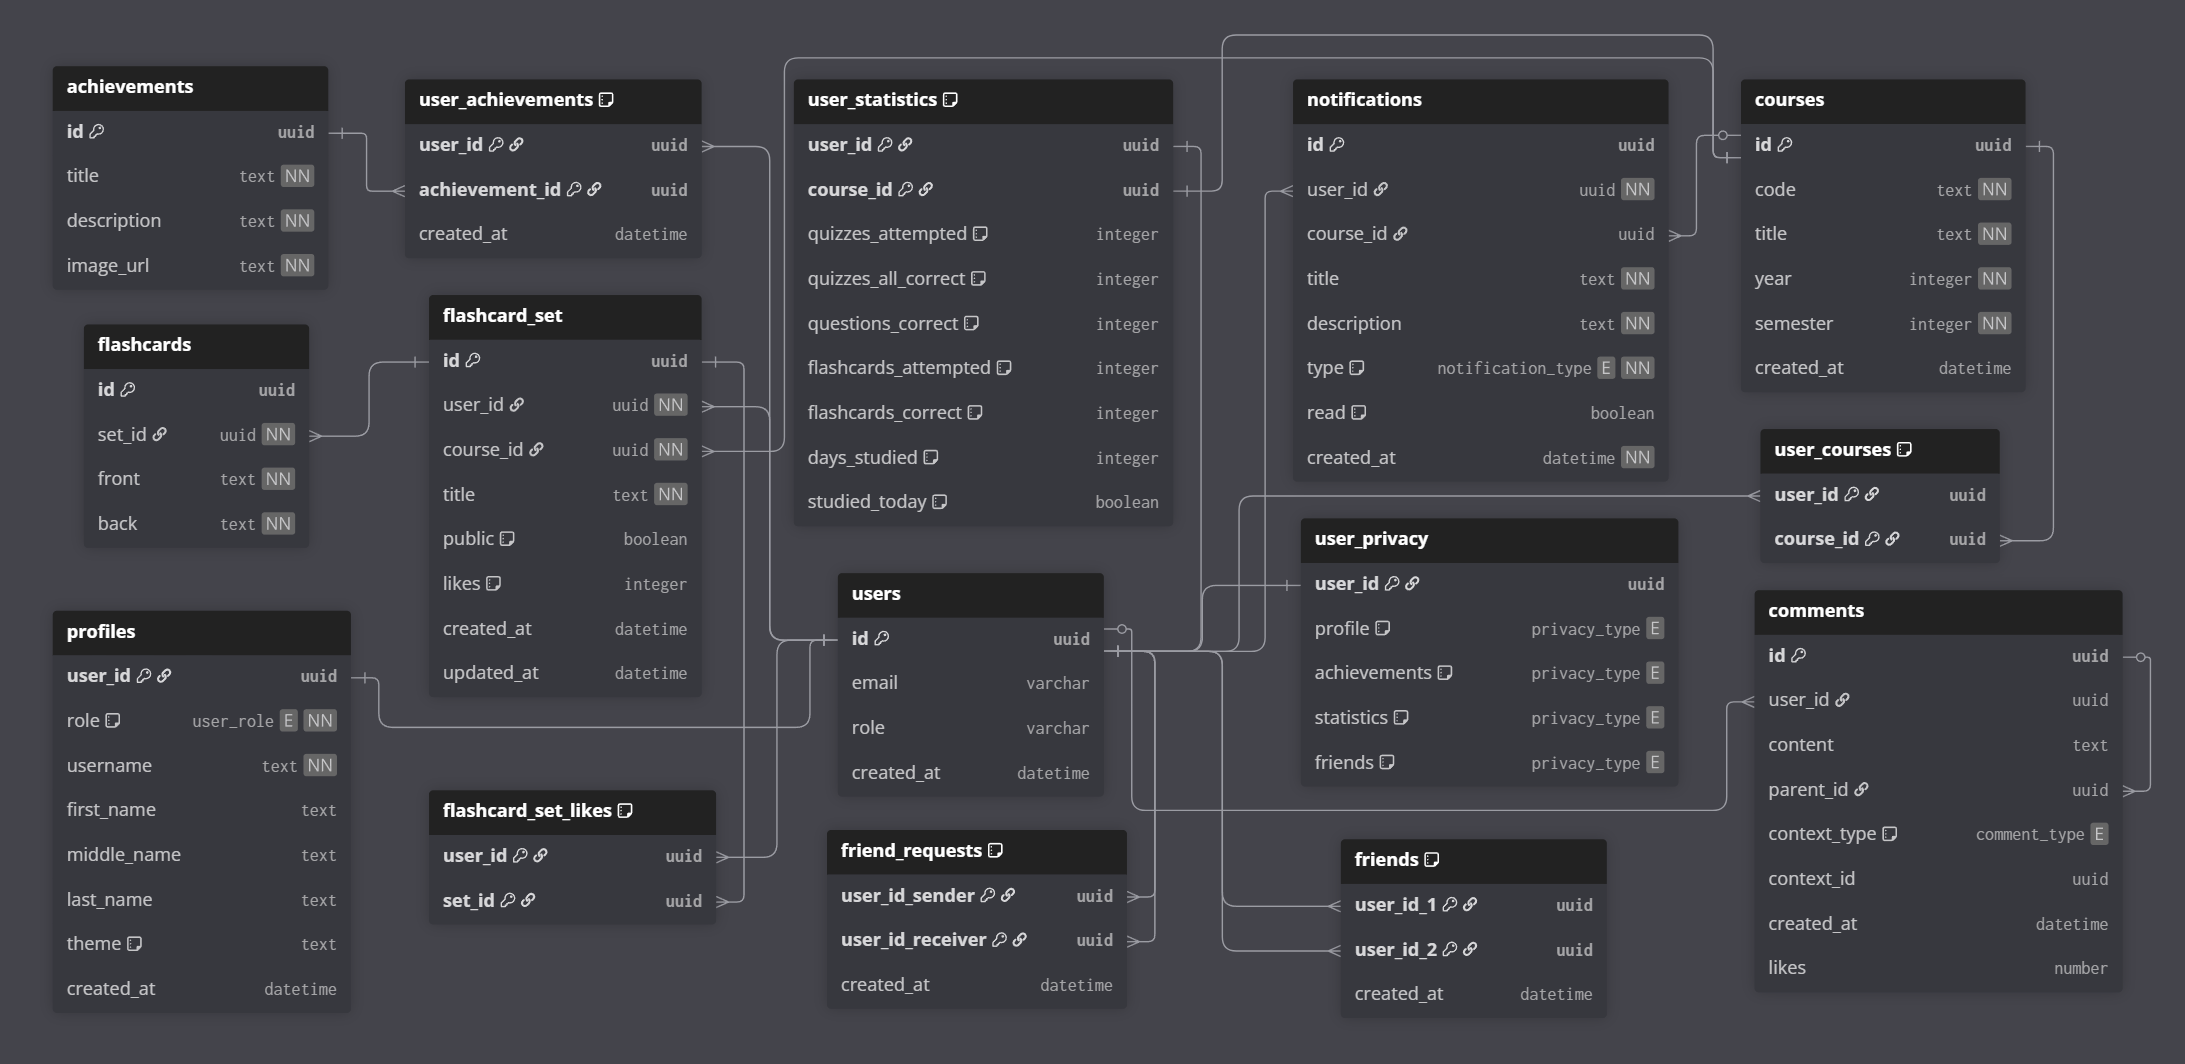
\includegraphics[width=\linewidth]{Planning/EarlyERD.png}
    \caption{Planned ER diagram for database}
    \label{fig:earlyERD}
\end{figure}

\section{Organisation Tools}

\subsection{Git}

\textcolor{magenta}{\textit{Discuss how GitHub is a standard, and its usefulness due to version history and branches}}

\subsection{Trello}

To organise the numerous features going into ReviXion, Trello will be used for its kanban board feature.
This allows for splitting up large ideas into smaller, more manageable cards that can be sorted into categories.
The main three categories I want to work around are 'Ideas', 'To-Do' and 'In Progress'.

The 'Ideas' category is used for cards that are very early in planning.
This could be due to a lack of foundation, or there is something stopping it from becoming a must-feature of the website.
They are very broad, conceptual, and highly susceptible to large changes.
The 'To-Do' category is used for ideas that have taken shape and are ready to start being implemented.
At this point, the original idea is split up into lots of smaller cards to deal with one by one.
The 'In Progress' category is self-explanatory, but is very useful for task-swapping.
If issues start to arise with one 'In Progress' task, it is very easy to put this on hold and take on another task instead.

\begin{figure}[H]
    \centering
    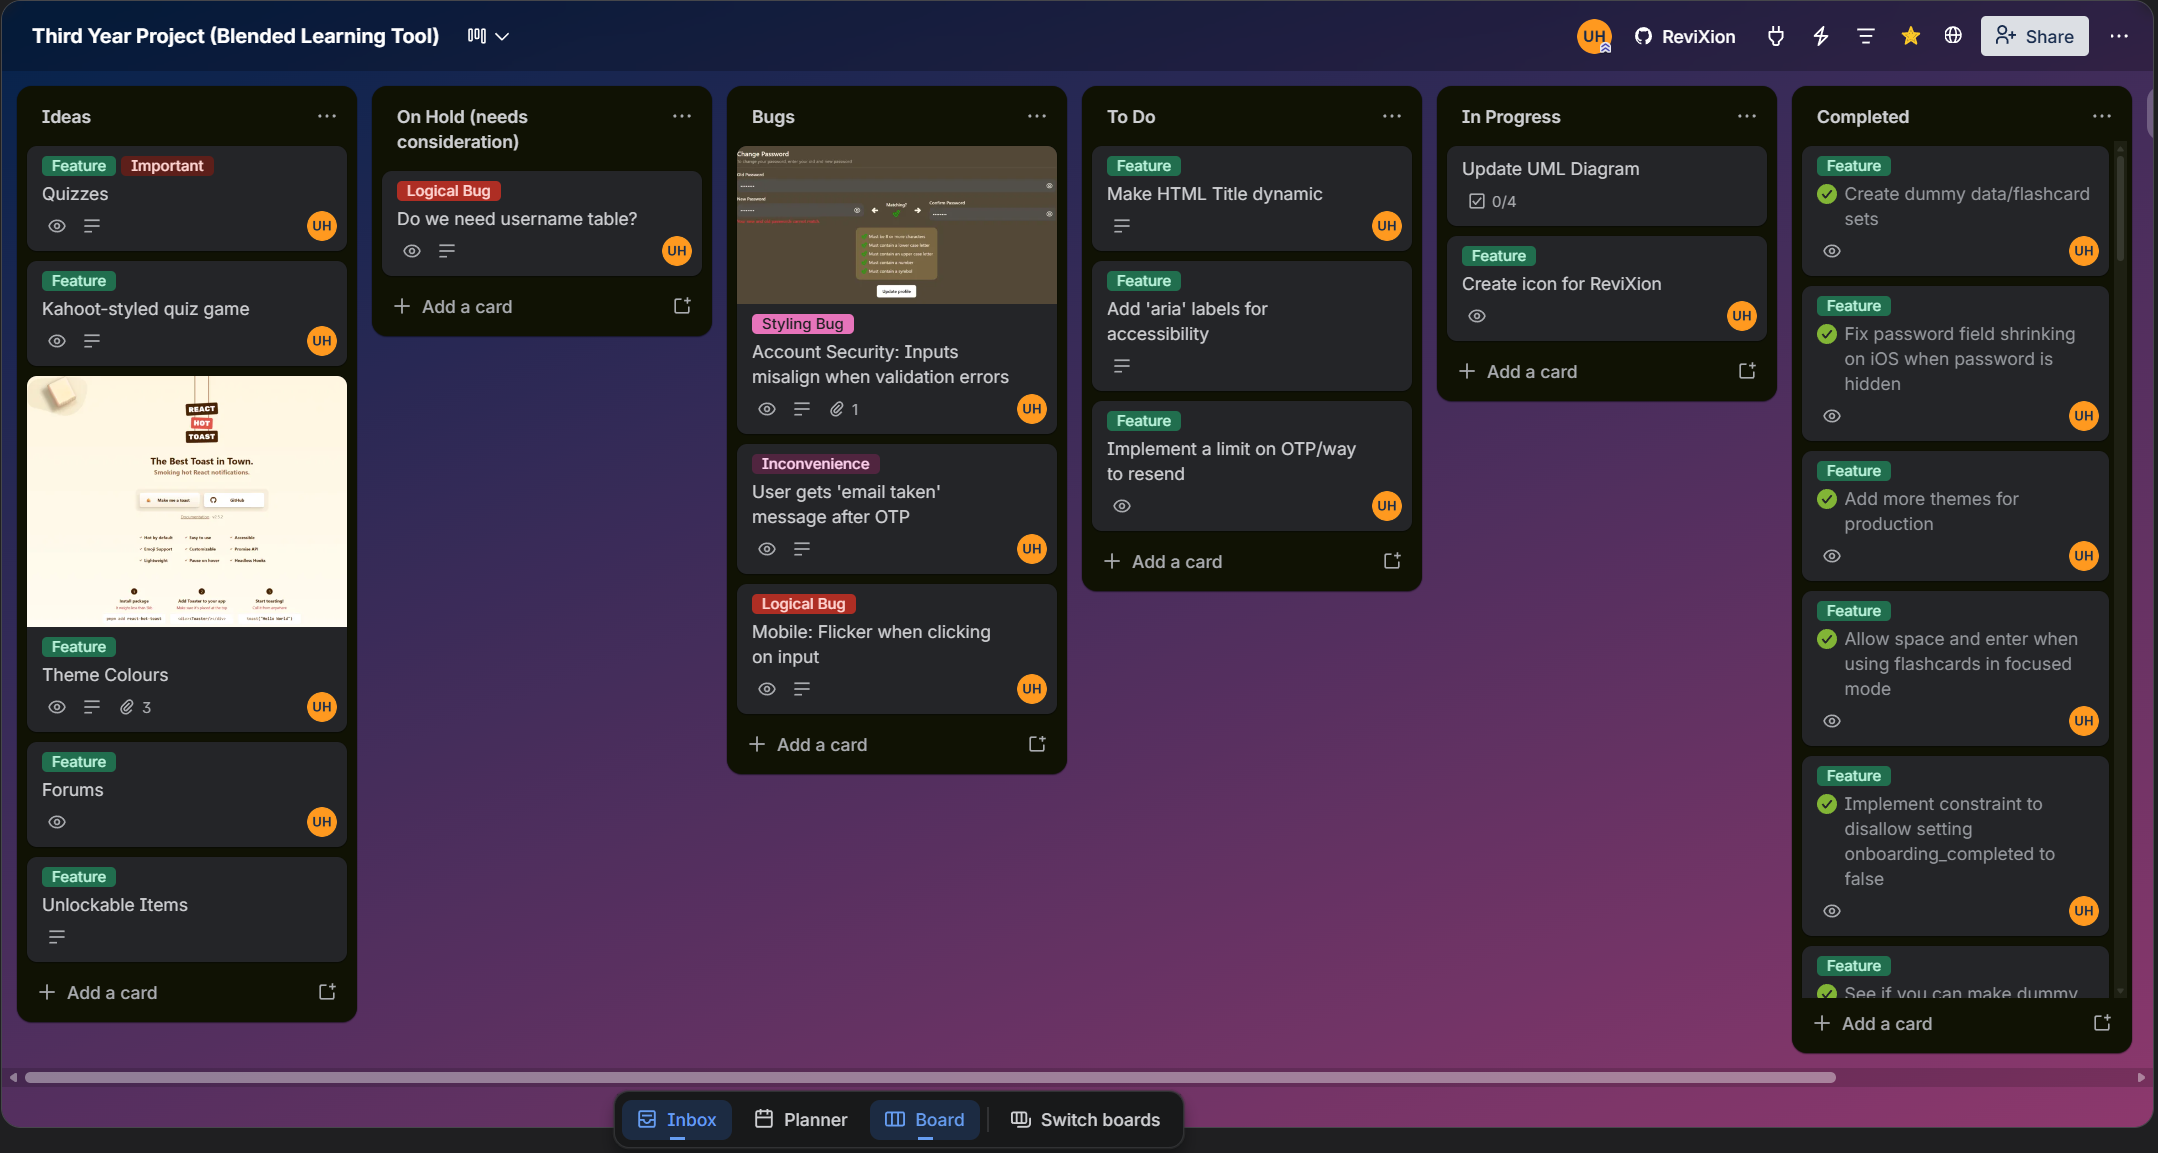
\includegraphics[width=\linewidth]{Planning/Trello.png}
    \caption{Trello Kanban Board showing each of the categories}
    \label{fig:trello}
\end{figure}

\begin{figure}[H]
    \centering
    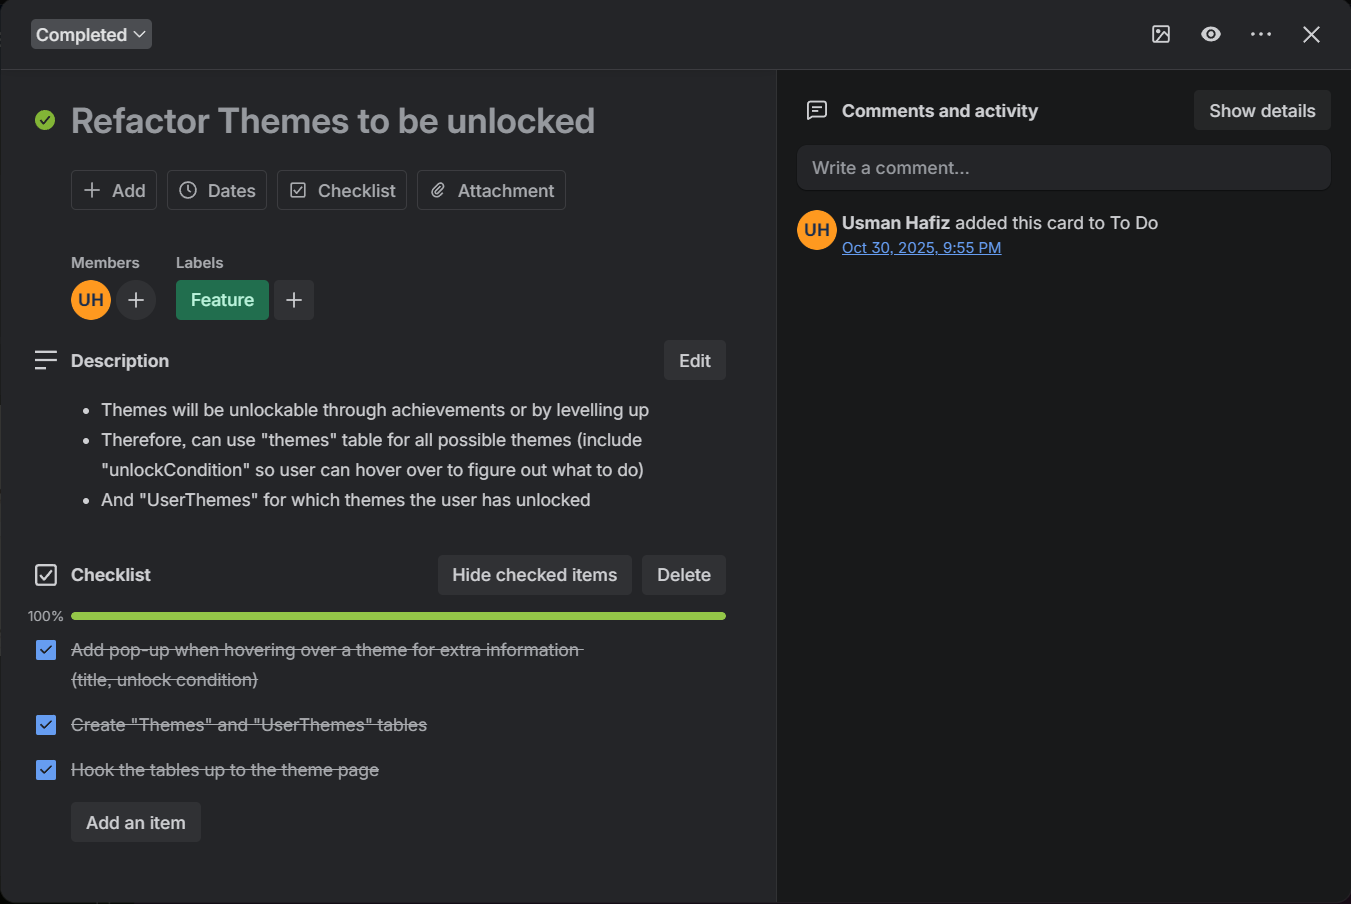
\includegraphics[width=\linewidth]{Planning/TrelloCard.png}
    \caption{An example of a completed Trello card}
    \label{fig:trelloCard}
\end{figure}

\chapter{Development and Implementation}

\textcolor{magenta}{\textit{Add proper introduction. How...?}}

\section{UI Design Principles}

The aim of the UI for ReviXion is that it must remain focused, whilst having enough expression to be 'attractive' to users.
Part of the attraction comes from the various themes on offer (see Figs. \ref{fig:lightThemes} and \ref{fig:darkThemes}).
Besides the themes, the UI needs to remain simple enough not to be distracting from the main purpose the website, which is, studying.

The result is a very simple UI which avoids clutter and tries to get users where they need to be as quick as possible.

\textcolor{magenta}{\textit{Add more? Talk about how other learning platforms are difficult to navigate?}}

\section{Supabase Implementation}

\textcolor{magenta}{\textit{Discuss how Supabase was used, including local development, and migrations. Also discuss the use of edge functions for security, and the final database.}}

\begin{figure}[H]
    \centering
    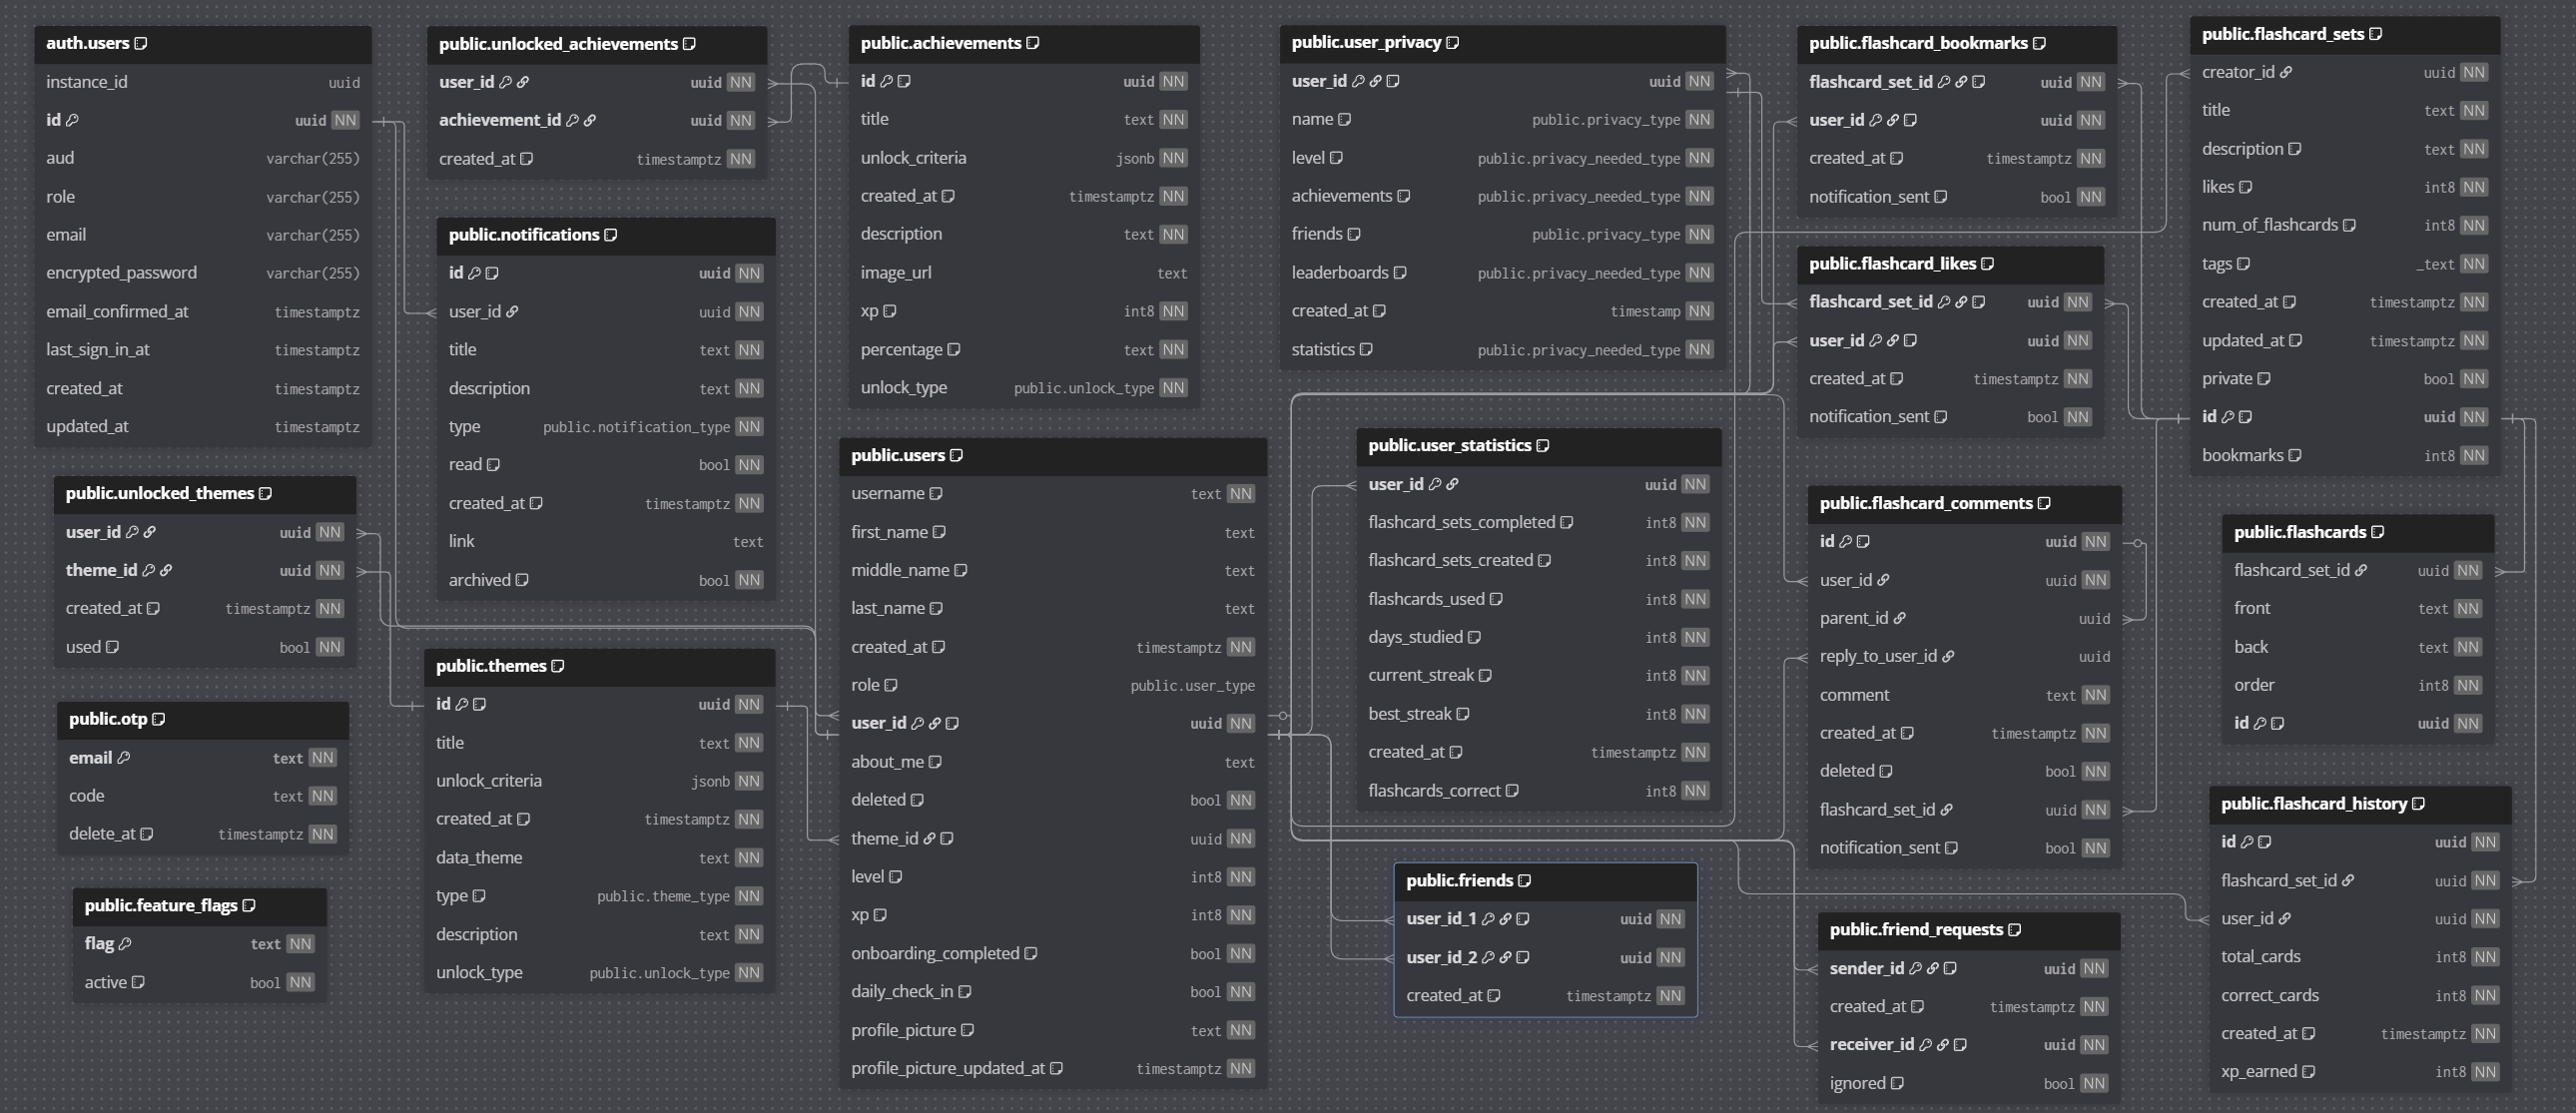
\includegraphics[width=\linewidth]{Planning/FinalERD.png}
    \caption{Final ER diagram for database after implementation}
    \label{fig:finalERD}
\end{figure}

\section{ReviXion Features}

\subsection{Onboarding Experience}

\textcolor{magenta}{\textit{Maybe cite something on the importance of a good onboarding experience?}}
When users first visit the website, they are greeted with a landing page explaining the key features of the website.
On other websites, signing up can sometimes be frustrating due to the large requirements for passwords without any feedback on if their password is matching these requirements.
This can be especially impactful if this is one of the first aspects of the website you encounter.
This is circumvented by giving the user live feedback on their password as they type with an intuitive UI.

\begin{figure}[H]
    \centering
    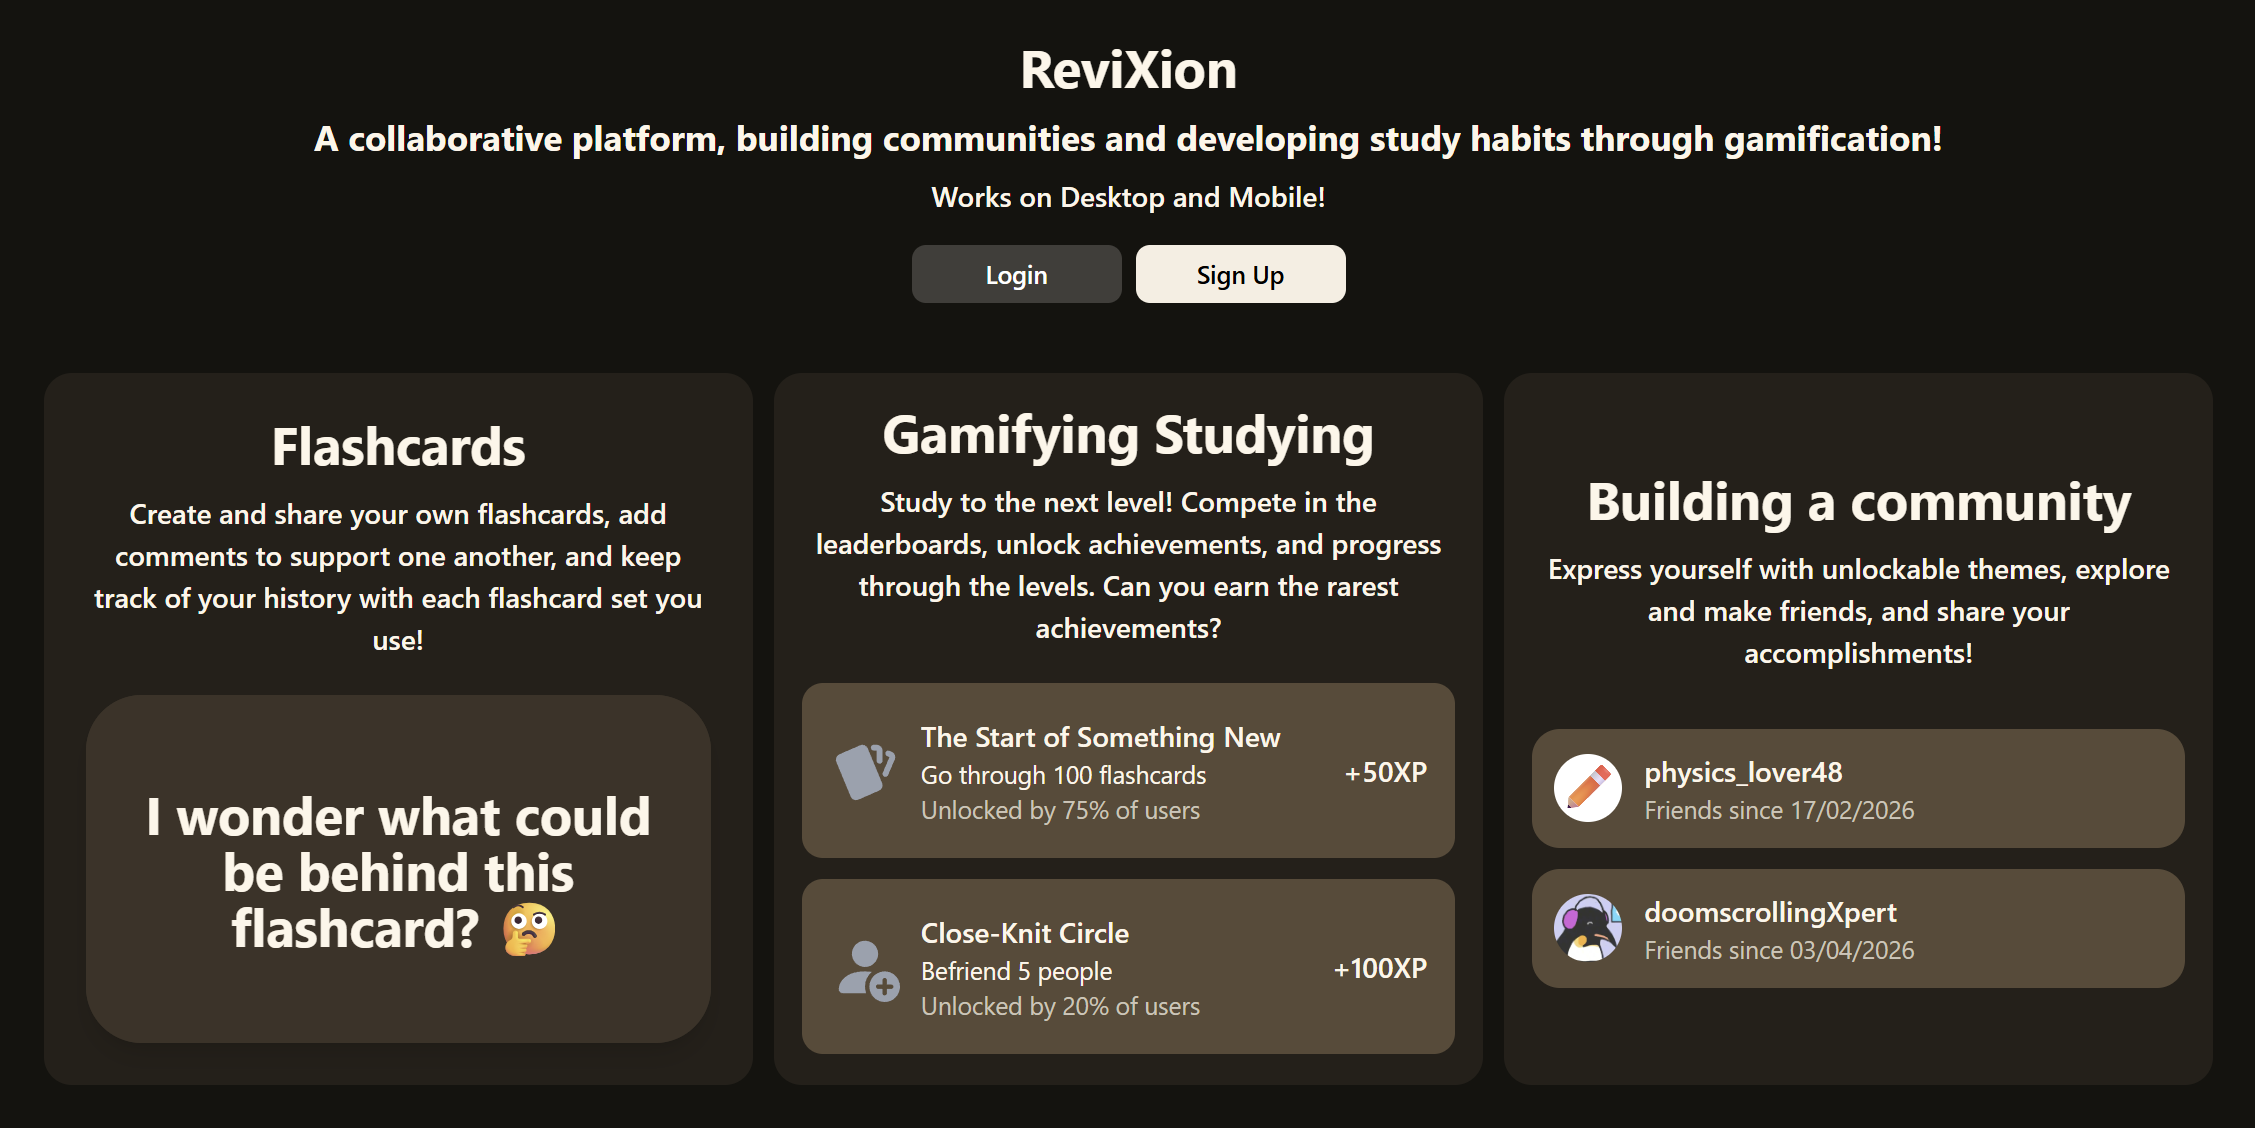
\includegraphics[width=\linewidth]{Implementation/Onboarding/LandingPage.png}
    \caption{Landing Page for ReviXion}
    \label{fig:landingPage}
\end{figure}

\begin{figure}[H]
    \centering
    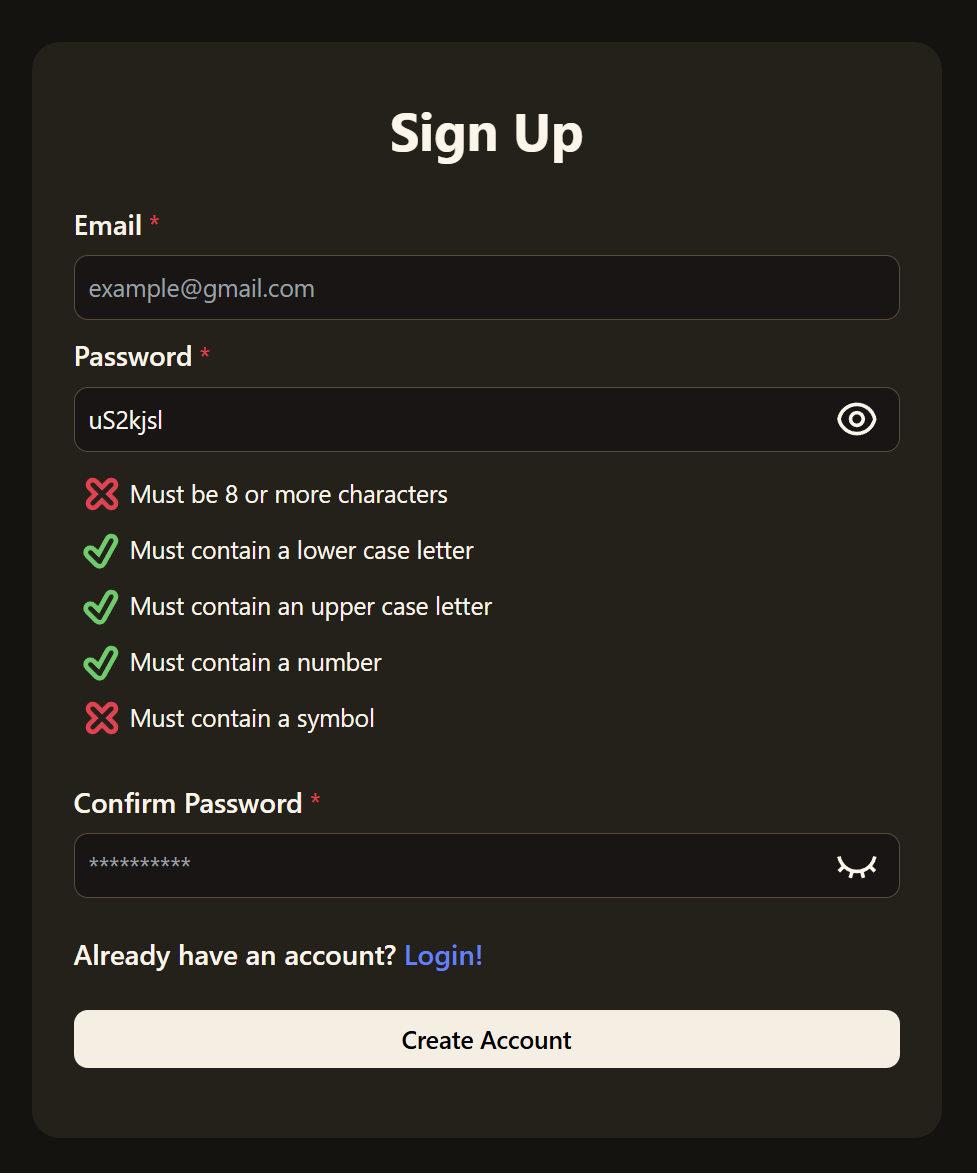
\includegraphics[width=0.5\linewidth]{Implementation/Onboarding/SignUpPage.png}
    \caption{Sign Up page, showing the password validation with an example password}
    \label{fig:signUpPage}
\end{figure}

To prevent users from inputting email addresses other than their own, a One Time Password (OTP) will be sent to their email.
They will then have to input this OTP to verify ownership of that email address and progress to the onboarding steps.
This is done as a way to prevent users from entering email addresses that are either incorrect, or that do not belong to them.

\begin{figure}[H]
    \centering
    \begin{subfigure}{0.48\textwidth}
        \centering
        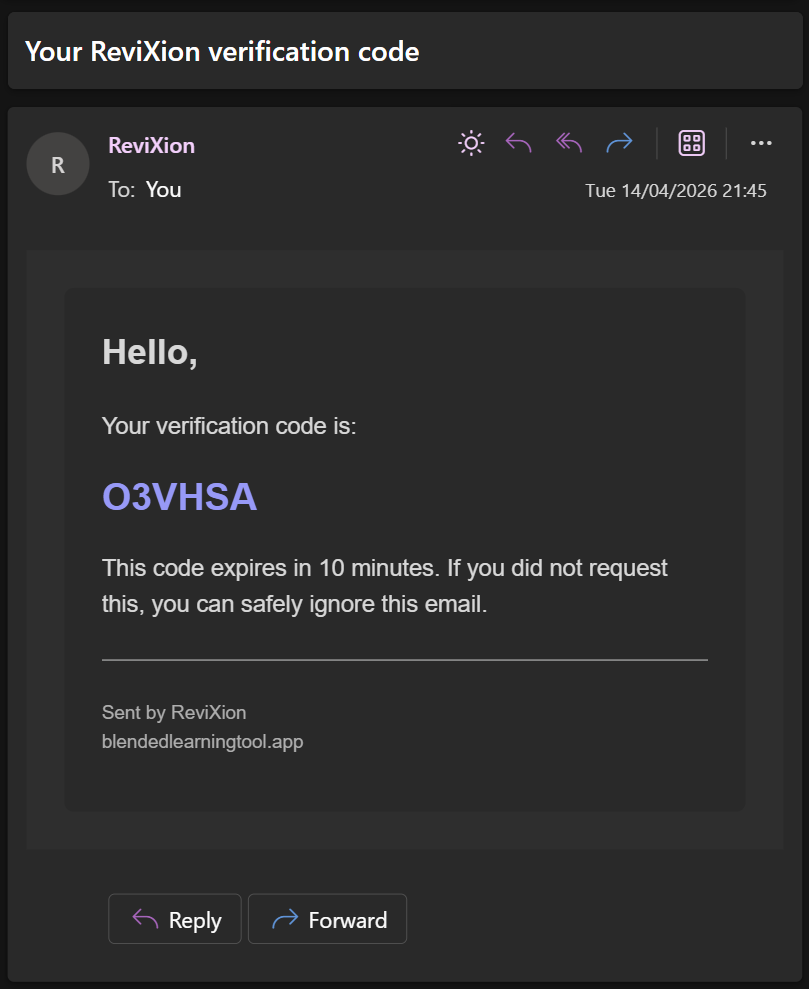
\includegraphics[width=\linewidth]{Implementation/Onboarding/OTPEmail.png}
        \caption{Email users receive containing OTP}
        \label{fig:otpEmail}
    \end{subfigure}
    \hfill
    \begin{subfigure}{0.48\textwidth}
        \centering
        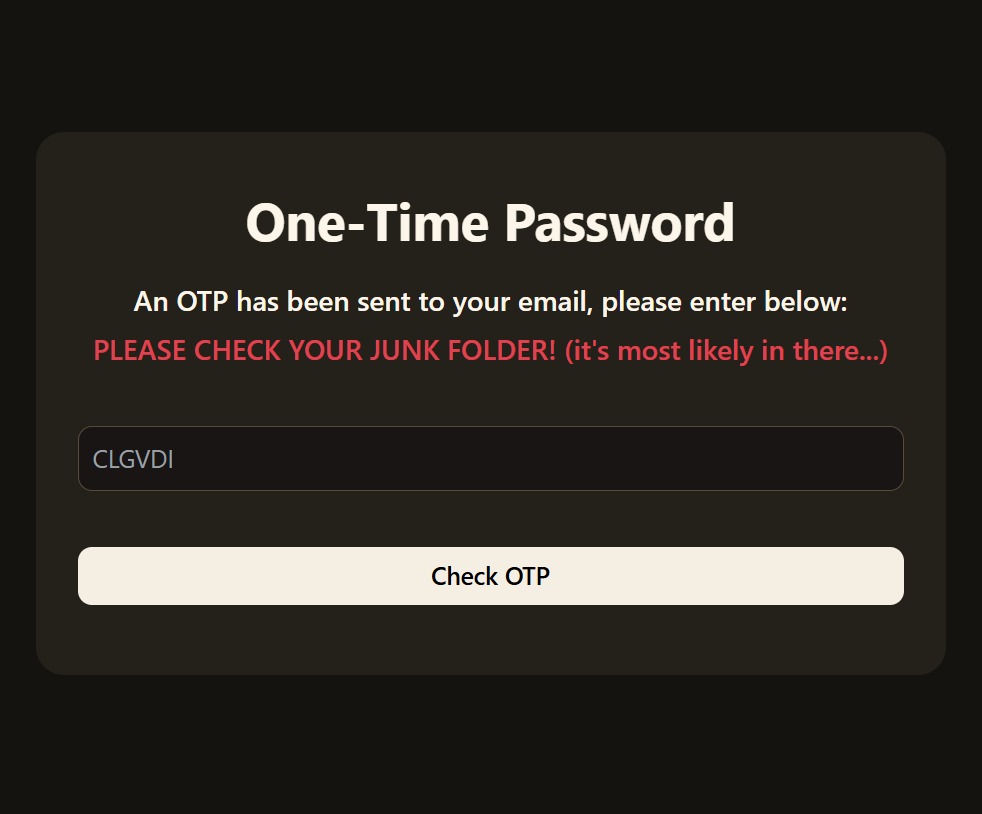
\includegraphics[width=\linewidth]{Implementation/Onboarding/OTPPage.png}
        \caption{OTP page}
        \label{fig:otpPage}
    \end{subfigure}
    \caption{One Time Password Functionality}
\end{figure}

The following onboarding steps give a quick run-through of a few features of the website.
These include the profile personalisations, profile picture, privacy settings, and themes.
This helps to give users an early understanding of the customisation features (see Section \ref{customisationOptions})
and some of the themes they can unlock (see Fig. \ref{fig:themes}).
If a user so wishes to sign out or accidentally closes the page during onboarding,
logging in will redirect them back to the onboarding flow to ensure that they fill out the necessary information.

\begin{figure}[H]
    \centering
    \begin{subfigure}{0.32\textwidth}
        \centering
        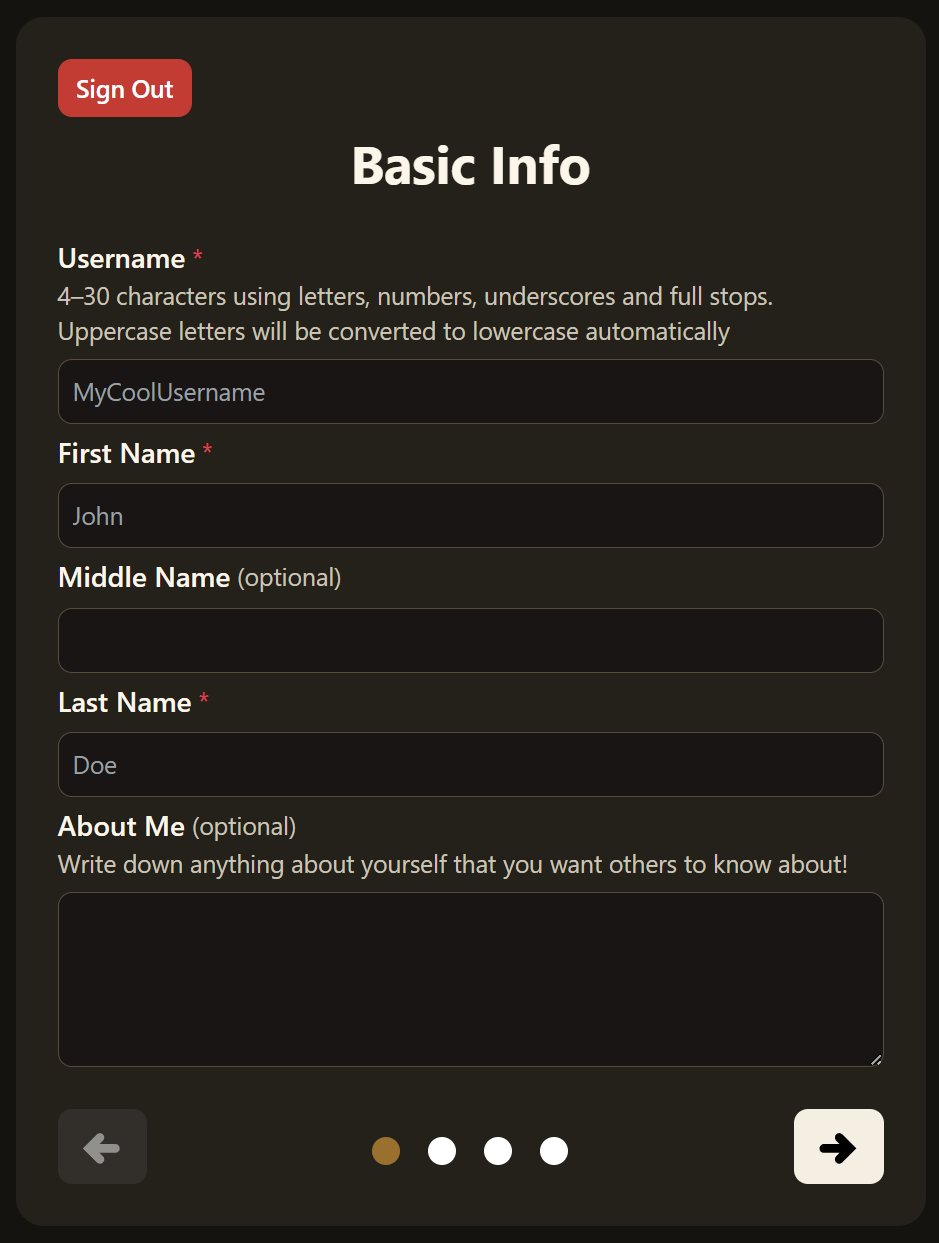
\includegraphics[width=\linewidth]{Implementation/Onboarding/ProfilePersonalisation.png}
        \caption{Basic Info}
        \label{fig:onboardingBasicInfo}
    \end{subfigure}
    \hfill
    \begin{subfigure}{0.32\textwidth}
        \centering
        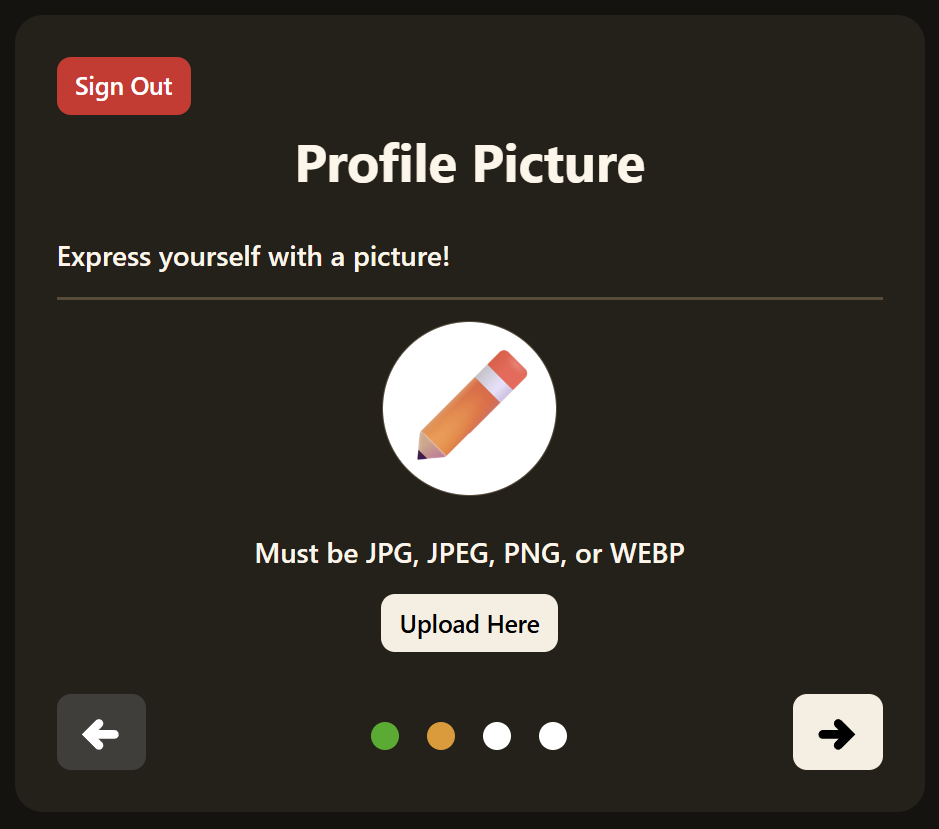
\includegraphics[width=\linewidth]{Implementation/Onboarding/ProfilePicture.png}
        \caption{Profile Picture}
        \label{fig:onboardingProfilePicture}
    \end{subfigure}
    \begin{subfigure}{0.32\textwidth}
        \centering
        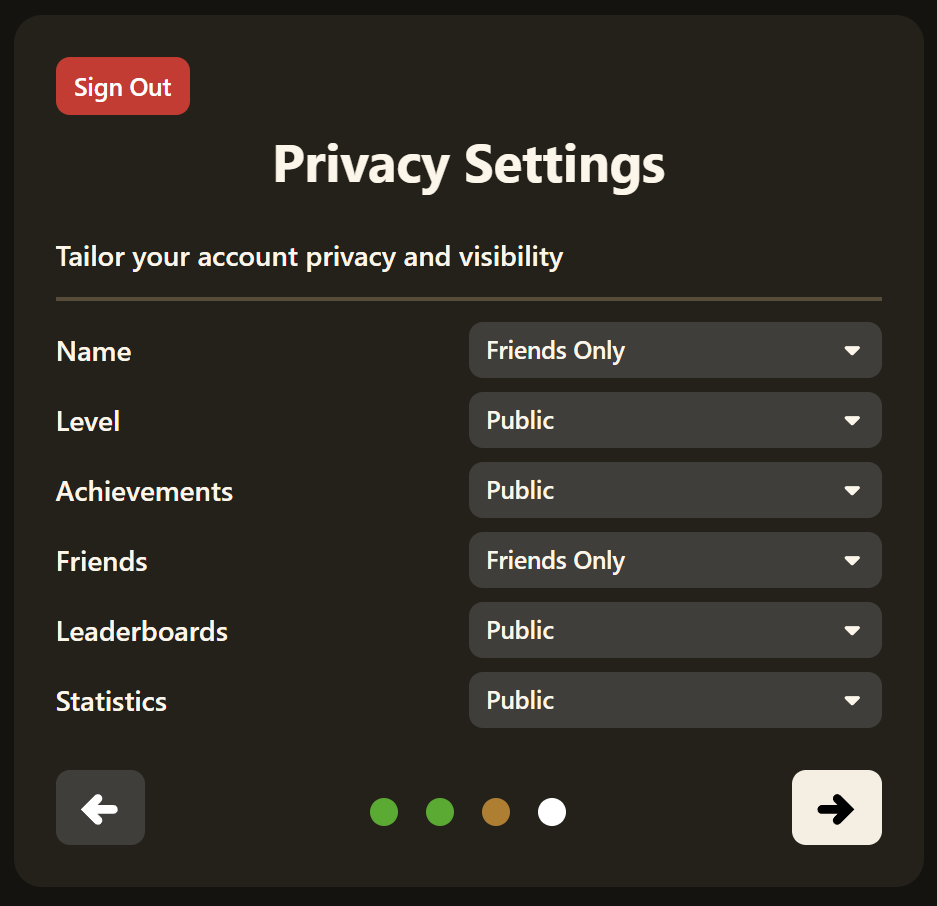
\includegraphics[width=\linewidth]{Implementation/Onboarding/PrivacySettings.png}
        \caption{Privacy Settings}
        \label{fig:onboardingPrivacySettings}
    \end{subfigure}
    \hfill
    \caption{Onboarding Pages}
\end{figure}

\subsection{Levels, Statistics and Leaderboards}

As part of the 'gamification' side of the website, each user has their own level,
and can increase their level by doing various tasks,
such as unlocking achievements (see Fig. \ref{fig:achievements}) or using flashcards (see Fig. \ref{fig:studyMode}).
Currently, levels are linear-based, meaning that it takes a fixed amount of XP to get to the next level.

An important way of levelling up is by checking in daily.
This encourages users to maintain more of a consistent engagement with the website and keep up a study streak, rather than visiting the website on very few occasions.

Similar to how video games have a running total of statistics that players can look back on,
ReviXion also features statistics for study methods, so that users can keep track of their progress and see just how much they have revised.

\begin{figure}[H]
    \centering
    \begin{subfigure}{\textwidth}
        \centering
        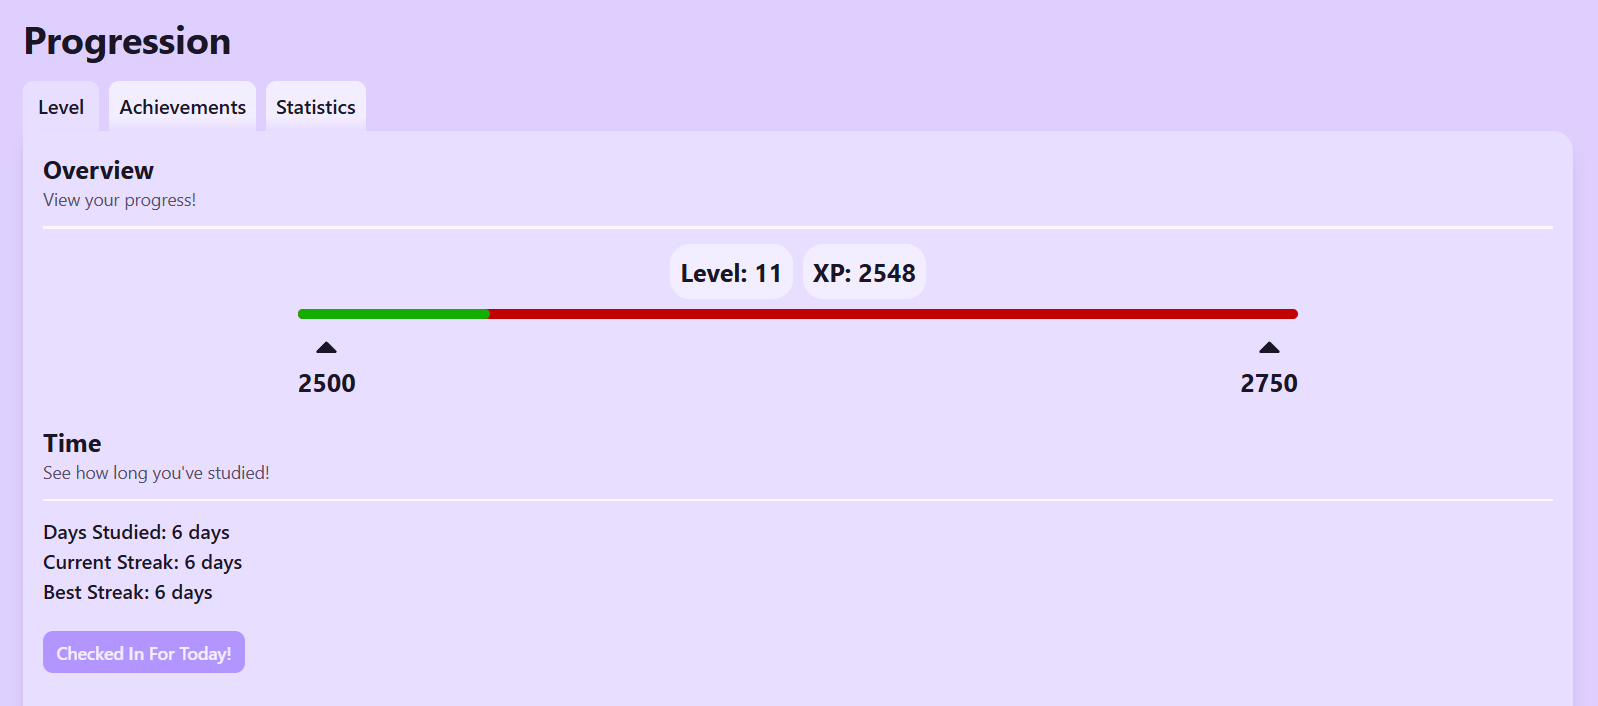
\includegraphics[width=\linewidth]{Implementation/Statistics/ProgressionTime.png}
        \caption{Level overview and daily check-in information}
        \label{fig:progressionTime}
    \end{subfigure}

    \vspace{0.5cm}

    \begin{subfigure}{\textwidth}
        \centering
        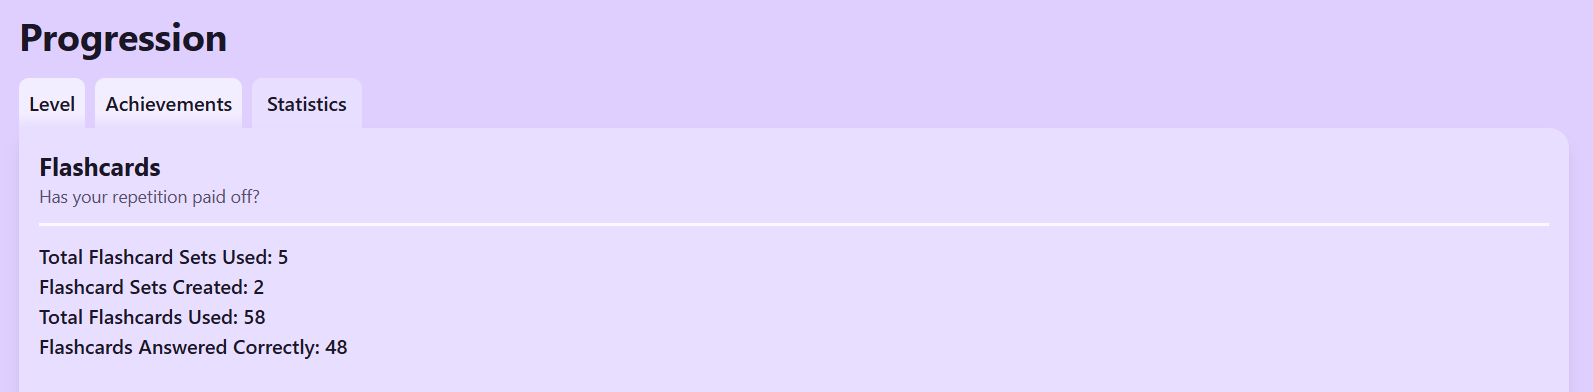
\includegraphics[width=\linewidth]{Implementation/Statistics/ProgressionStatistics.png}
        \caption{Accumulated statistics}
        \label{fig:progressionStatistics}
    \end{subfigure}

    \caption{'Progression' pages, where most of the 'gamification' aspects are located}
\end{figure}

Users can view their rankings against other users based on various statistics through the leaderboards.
Some examples of statistics include 'Days Studied', 'Flashcards Used' and 'Flashcard Sets Completed'.
Users can also filter the leaderboard to only include their friends, which may help to encourage groups of friends to study together and beat each others' statistics.

\begin{figure}[H]
    \centering
    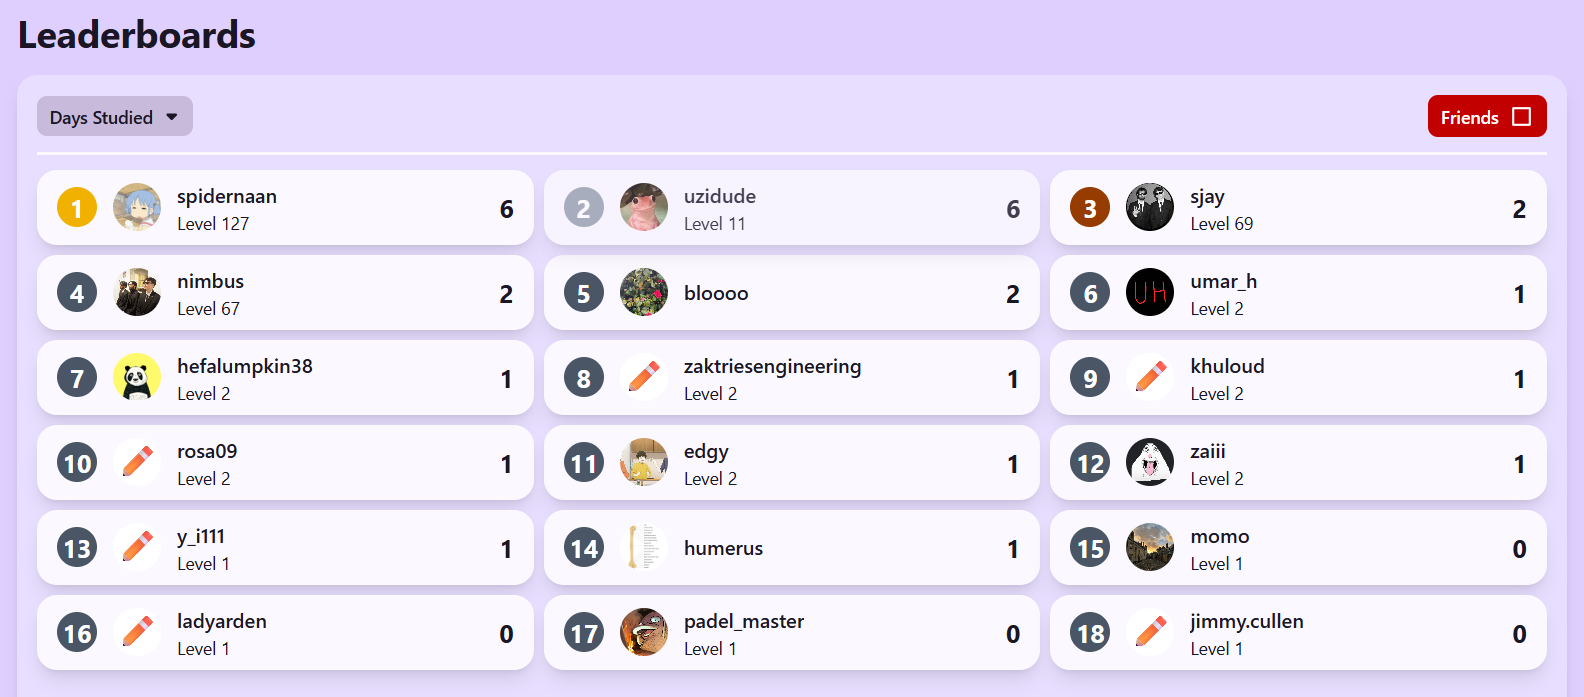
\includegraphics[width=\linewidth]{Implementation/Leaderboards/LeaderboardsDaysStudied.png}
    \caption{Leaderboard: Ranked by Days Studied}
    \label{fig:leaderboardsDaysStudied}
\end{figure}

\begin{figure}[H]
    \centering
    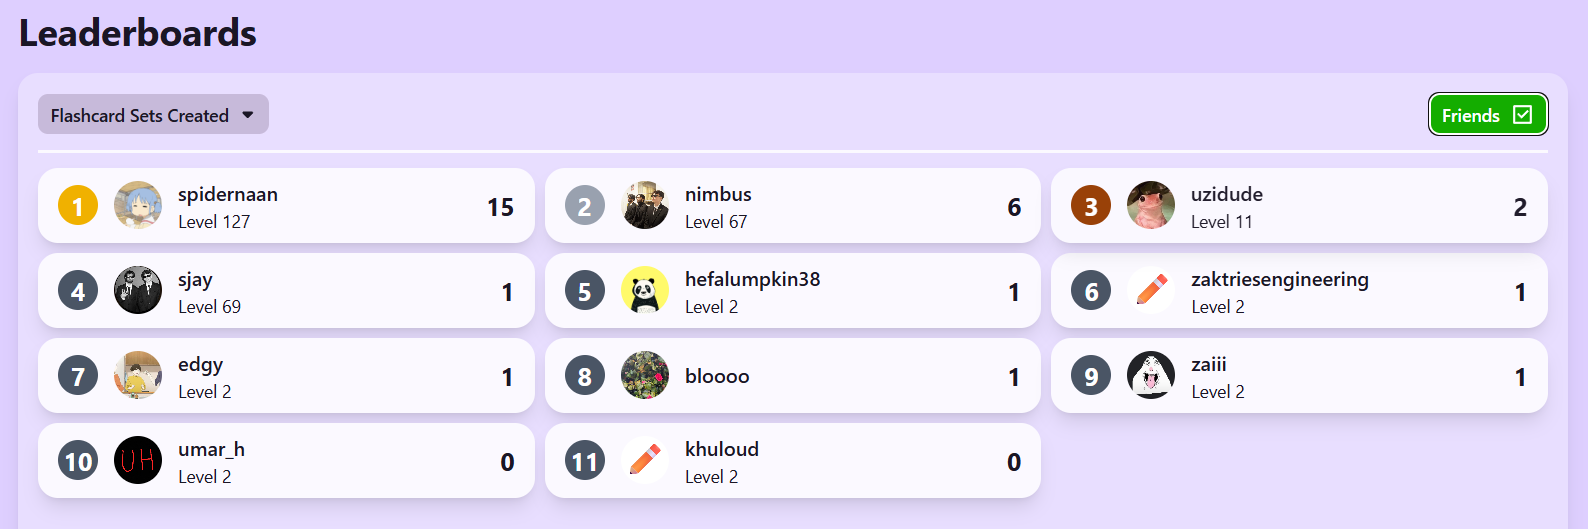
\includegraphics[width=\linewidth]{Implementation/Leaderboards/LeaderboardsFlashcardSetsCreated.png}
    \caption{Leaderboard: Ranked by Flashcard Sets Created (friends only)}
    \label{fig:leaderboardsFlashcardSetsCreated}
\end{figure}

\subsection{Customisation Options} \label{customisationOptions}

When users sign up, they are immediately given options to customise their profile.
They can add an 'About Me' to let other users know more about themselves.
They can also upload their own profile picture to express themselves further.
Finally, they can choose from various themes to customise the look of the website and choose the theme that fits best for them.
Each colour palette has both a light and dark variant as to give more flexibility on choice.

\begin{figure}[H]
    \centering
    
    \begin{subfigure}{\textwidth}
        \centering
        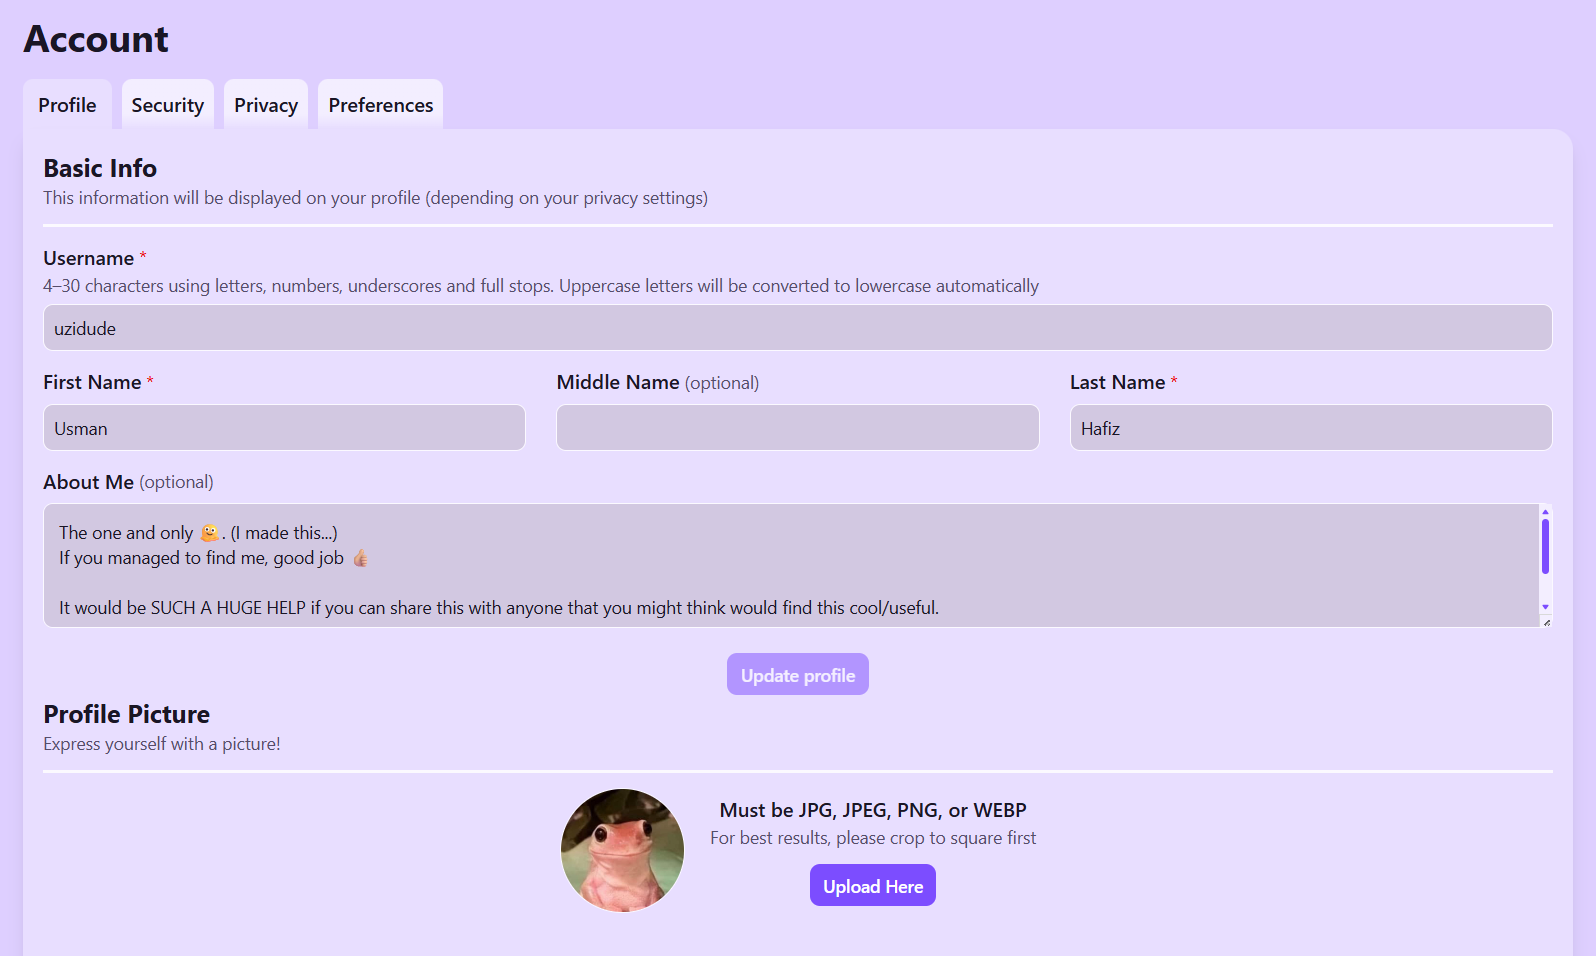
\includegraphics[width=\linewidth, keepaspectratio]{Implementation/ProfilePicture/BasicInfoAndUploadPfp.png}
        \caption{Updating account information}
        \label{fig:basicInfoAndUploadPfp}
    \end{subfigure}

    \vspace{0.5cm}

    \begin{subfigure}{\textwidth}
        \centering
        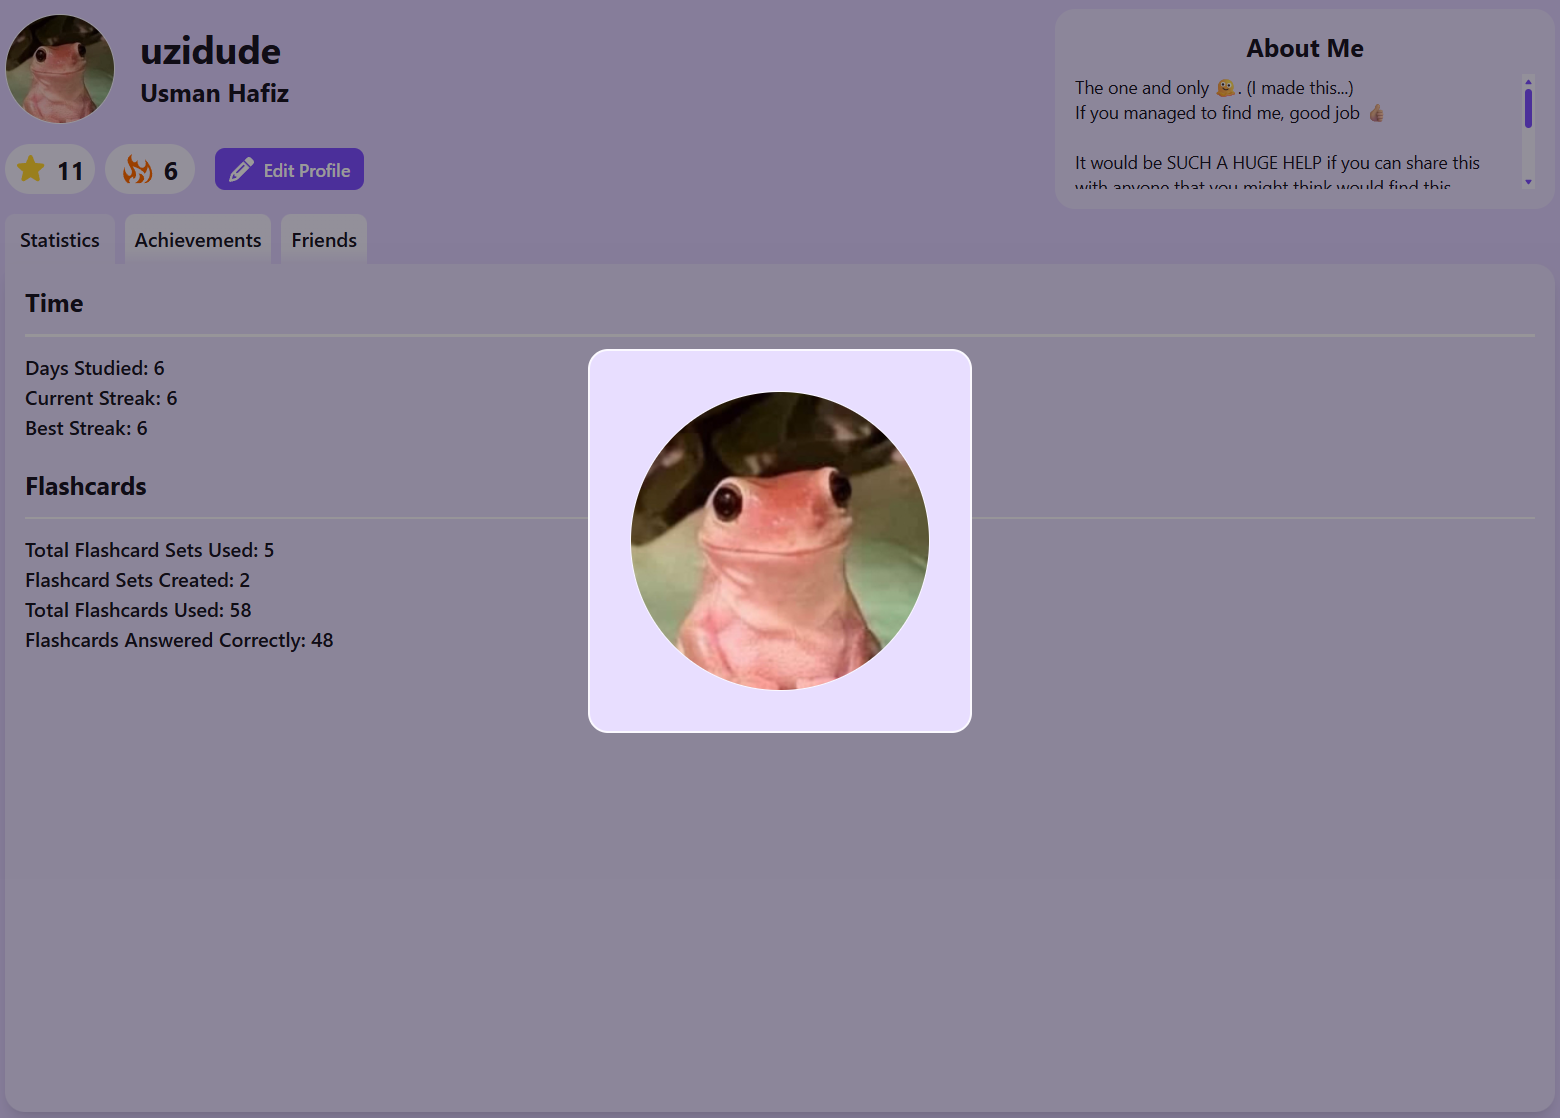
\includegraphics[width=\linewidth, keepaspectratio]{Implementation/ProfilePicture/CloseUpPfp.png}
        \caption{Viewing information and profile picture on user profiles}
        \label{fig:closeUpPfp}
    \end{subfigure}
    
    \caption{Account customisation functionality}
\end{figure}

\begin{figure}[H]
    \centering
    \begin{subfigure}{0.9\textwidth}
        \centering
        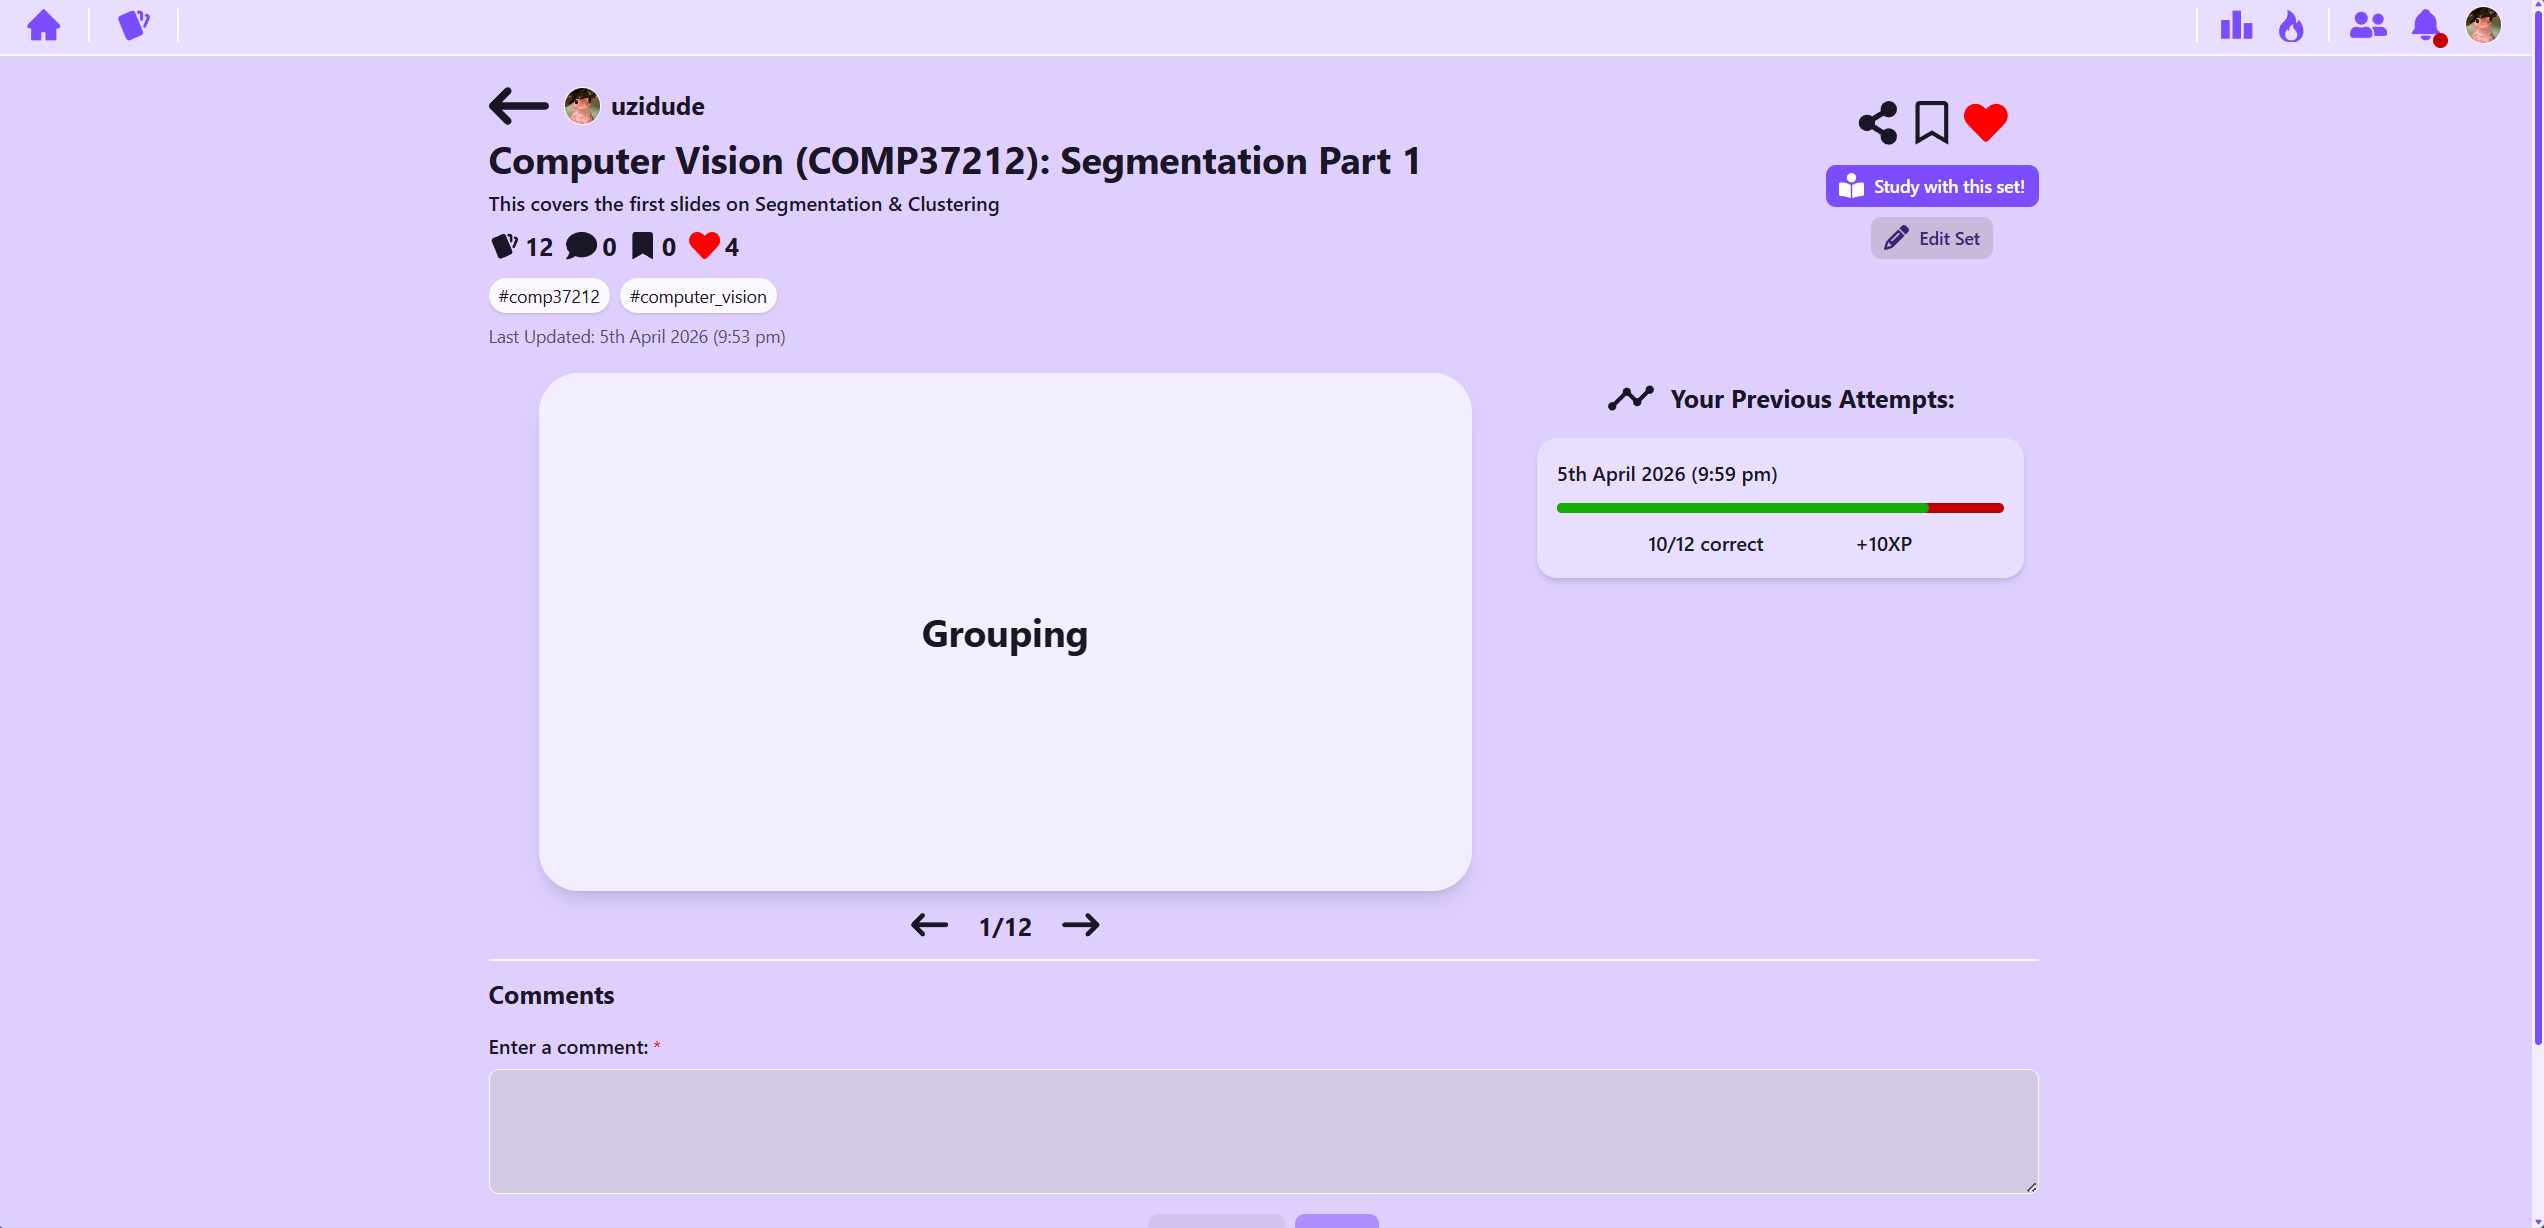
\includegraphics[width=\linewidth, keepaspectratio]{Implementation/Themes/Lavender.png}
        \caption{Lavender}
        \label{fig:lavender}
    \end{subfigure}
    
    \vspace{0.5cm}
    
    \begin{subfigure}{0.9\textwidth}
        \centering
        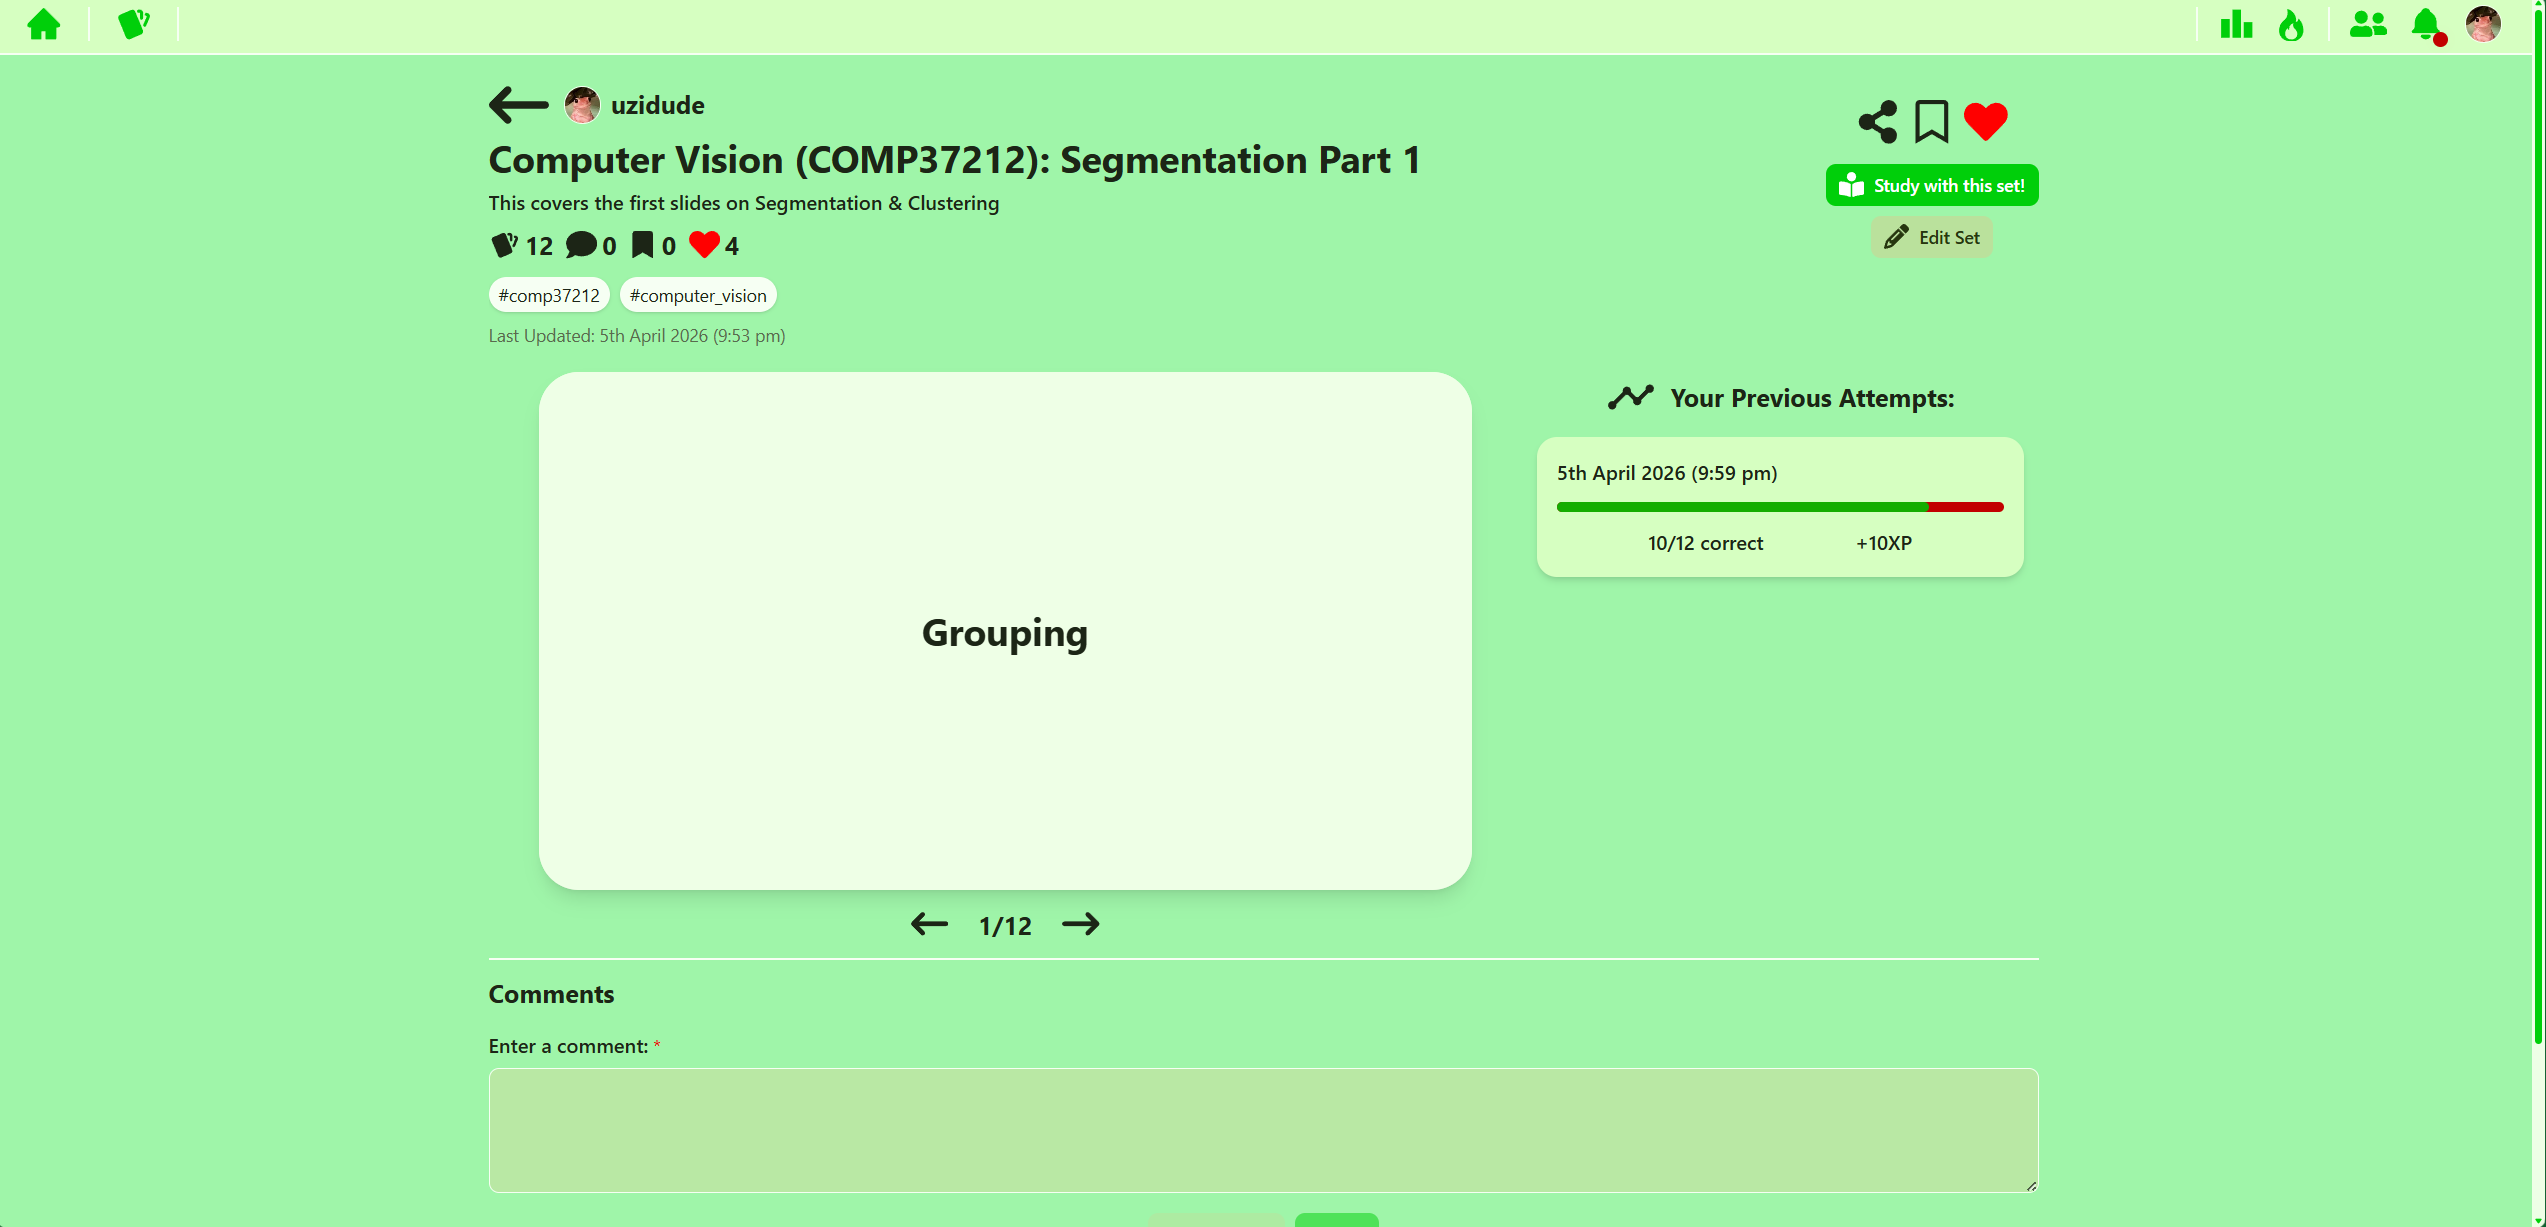
\includegraphics[width=\linewidth, keepaspectratio]{Implementation/Themes/Lemongrass.png}
        \caption{Lemongrass}
        \label{fig:lemongrass}
    \end{subfigure}
    
    \vspace{0.5cm}
    
    \begin{subfigure}{0.9\textwidth}
        \centering
        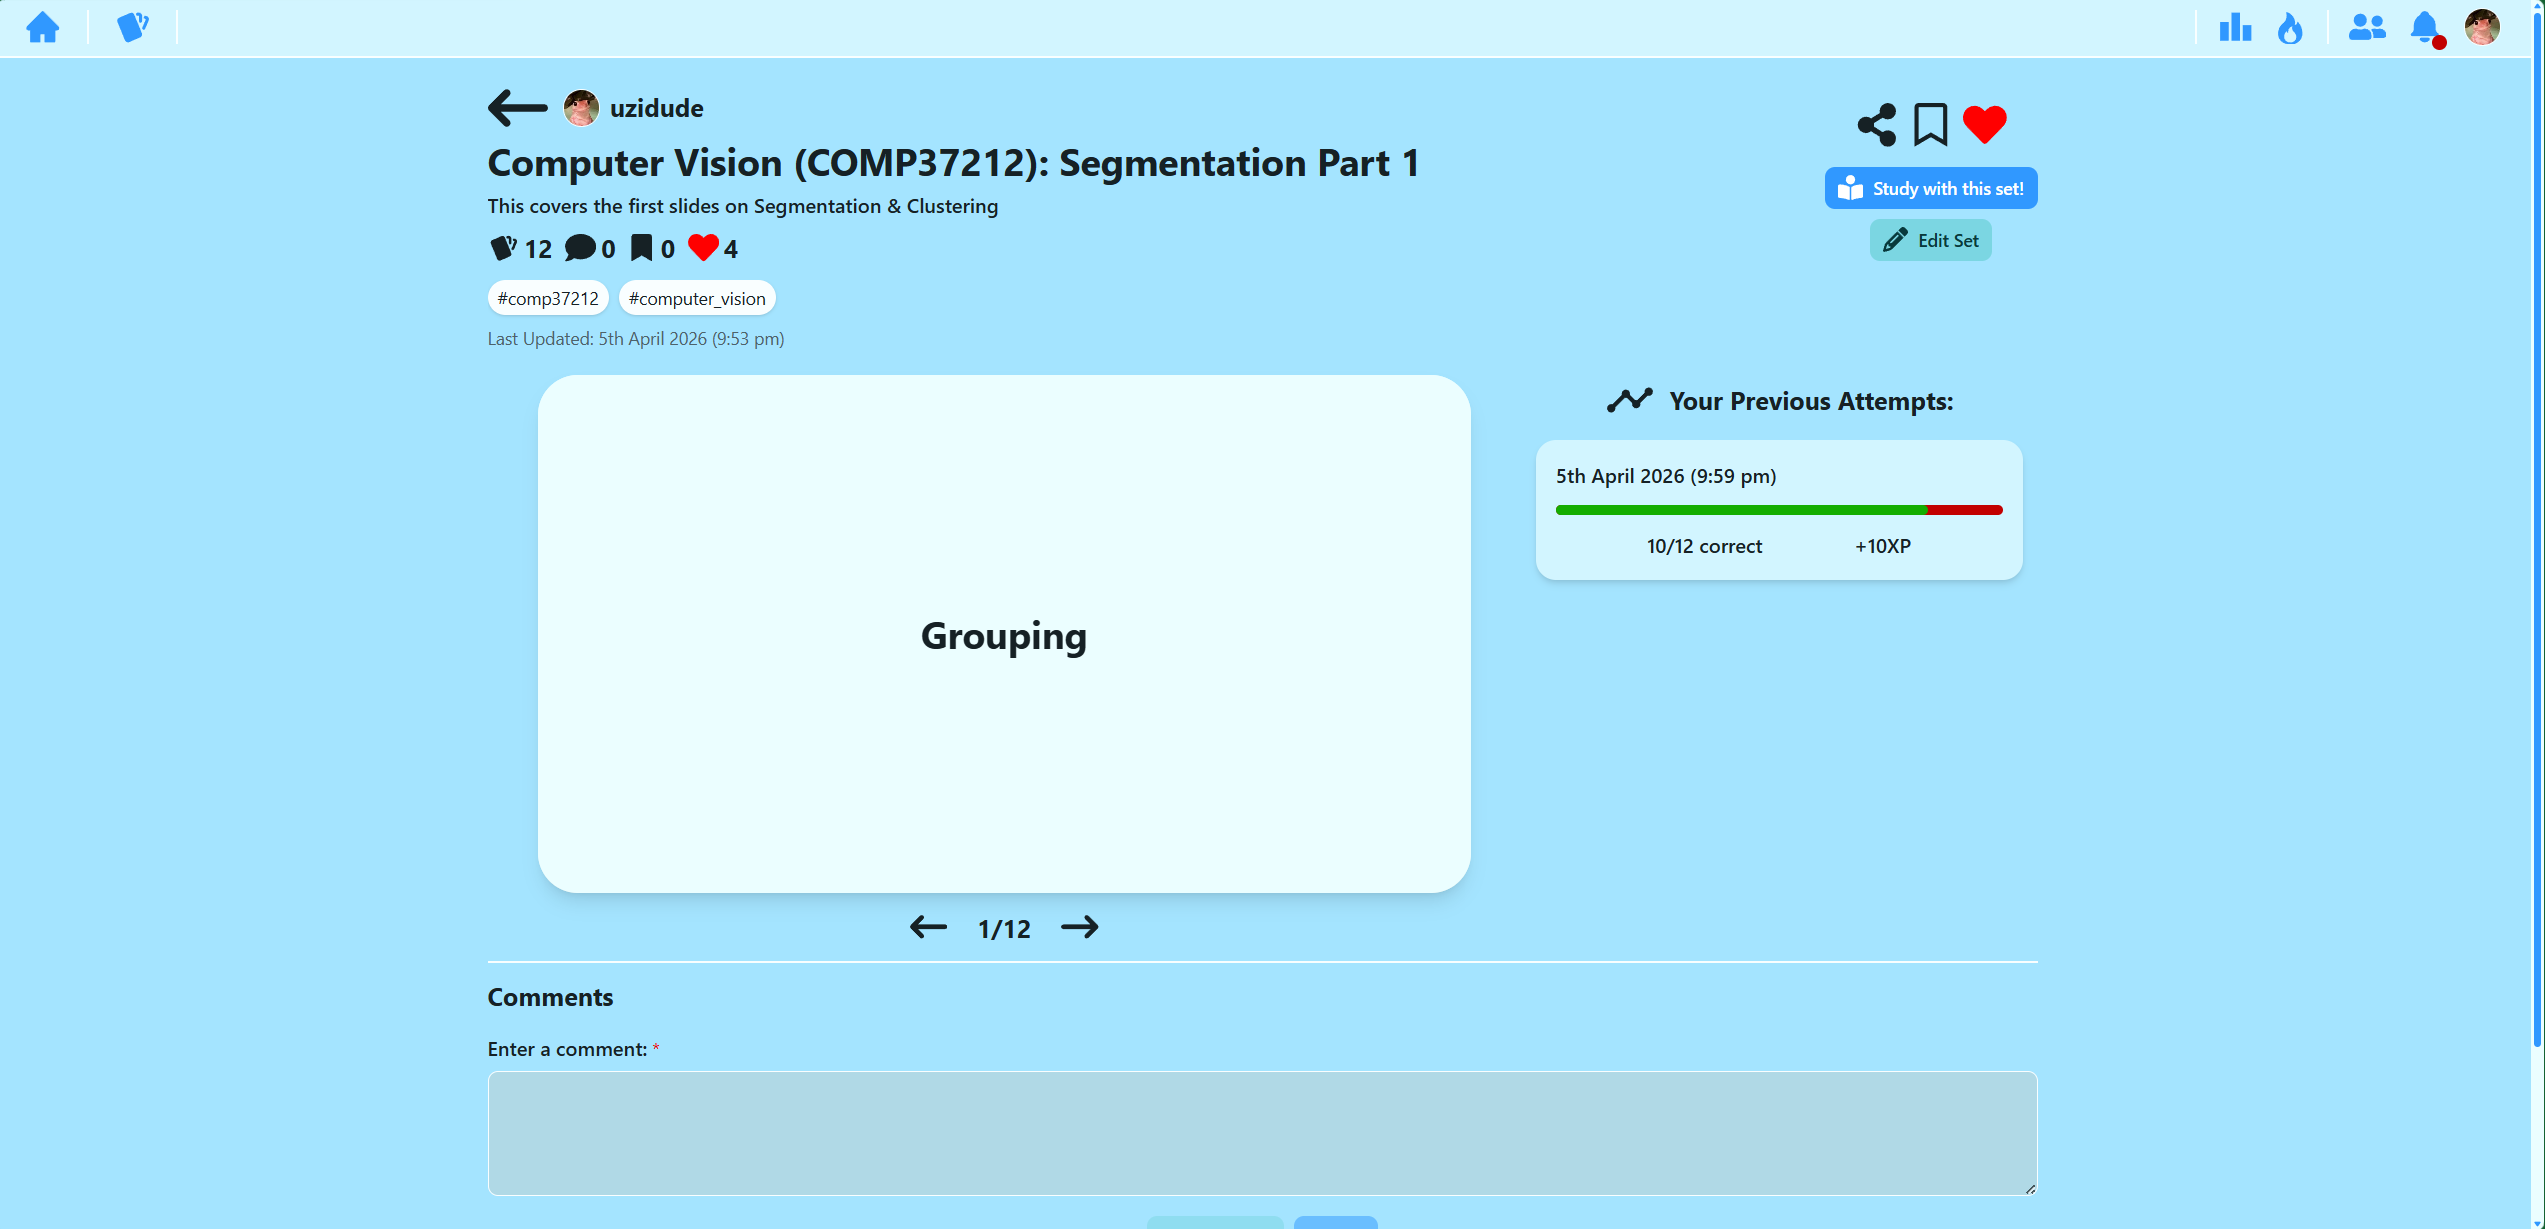
\includegraphics[width=\linewidth, keepaspectratio]{Implementation/Themes/SkyBlue.png}
        \caption{Sky Blue}
        \label{fig:skyBlue}
    \end{subfigure}
    \caption{A selection of the light themes, shown on the flashcard set overview page}
    \label{fig:lightThemes}
\end{figure}

\begin{figure}[H]
    \centering
    \begin{subfigure}{0.9\textwidth}
        \centering
        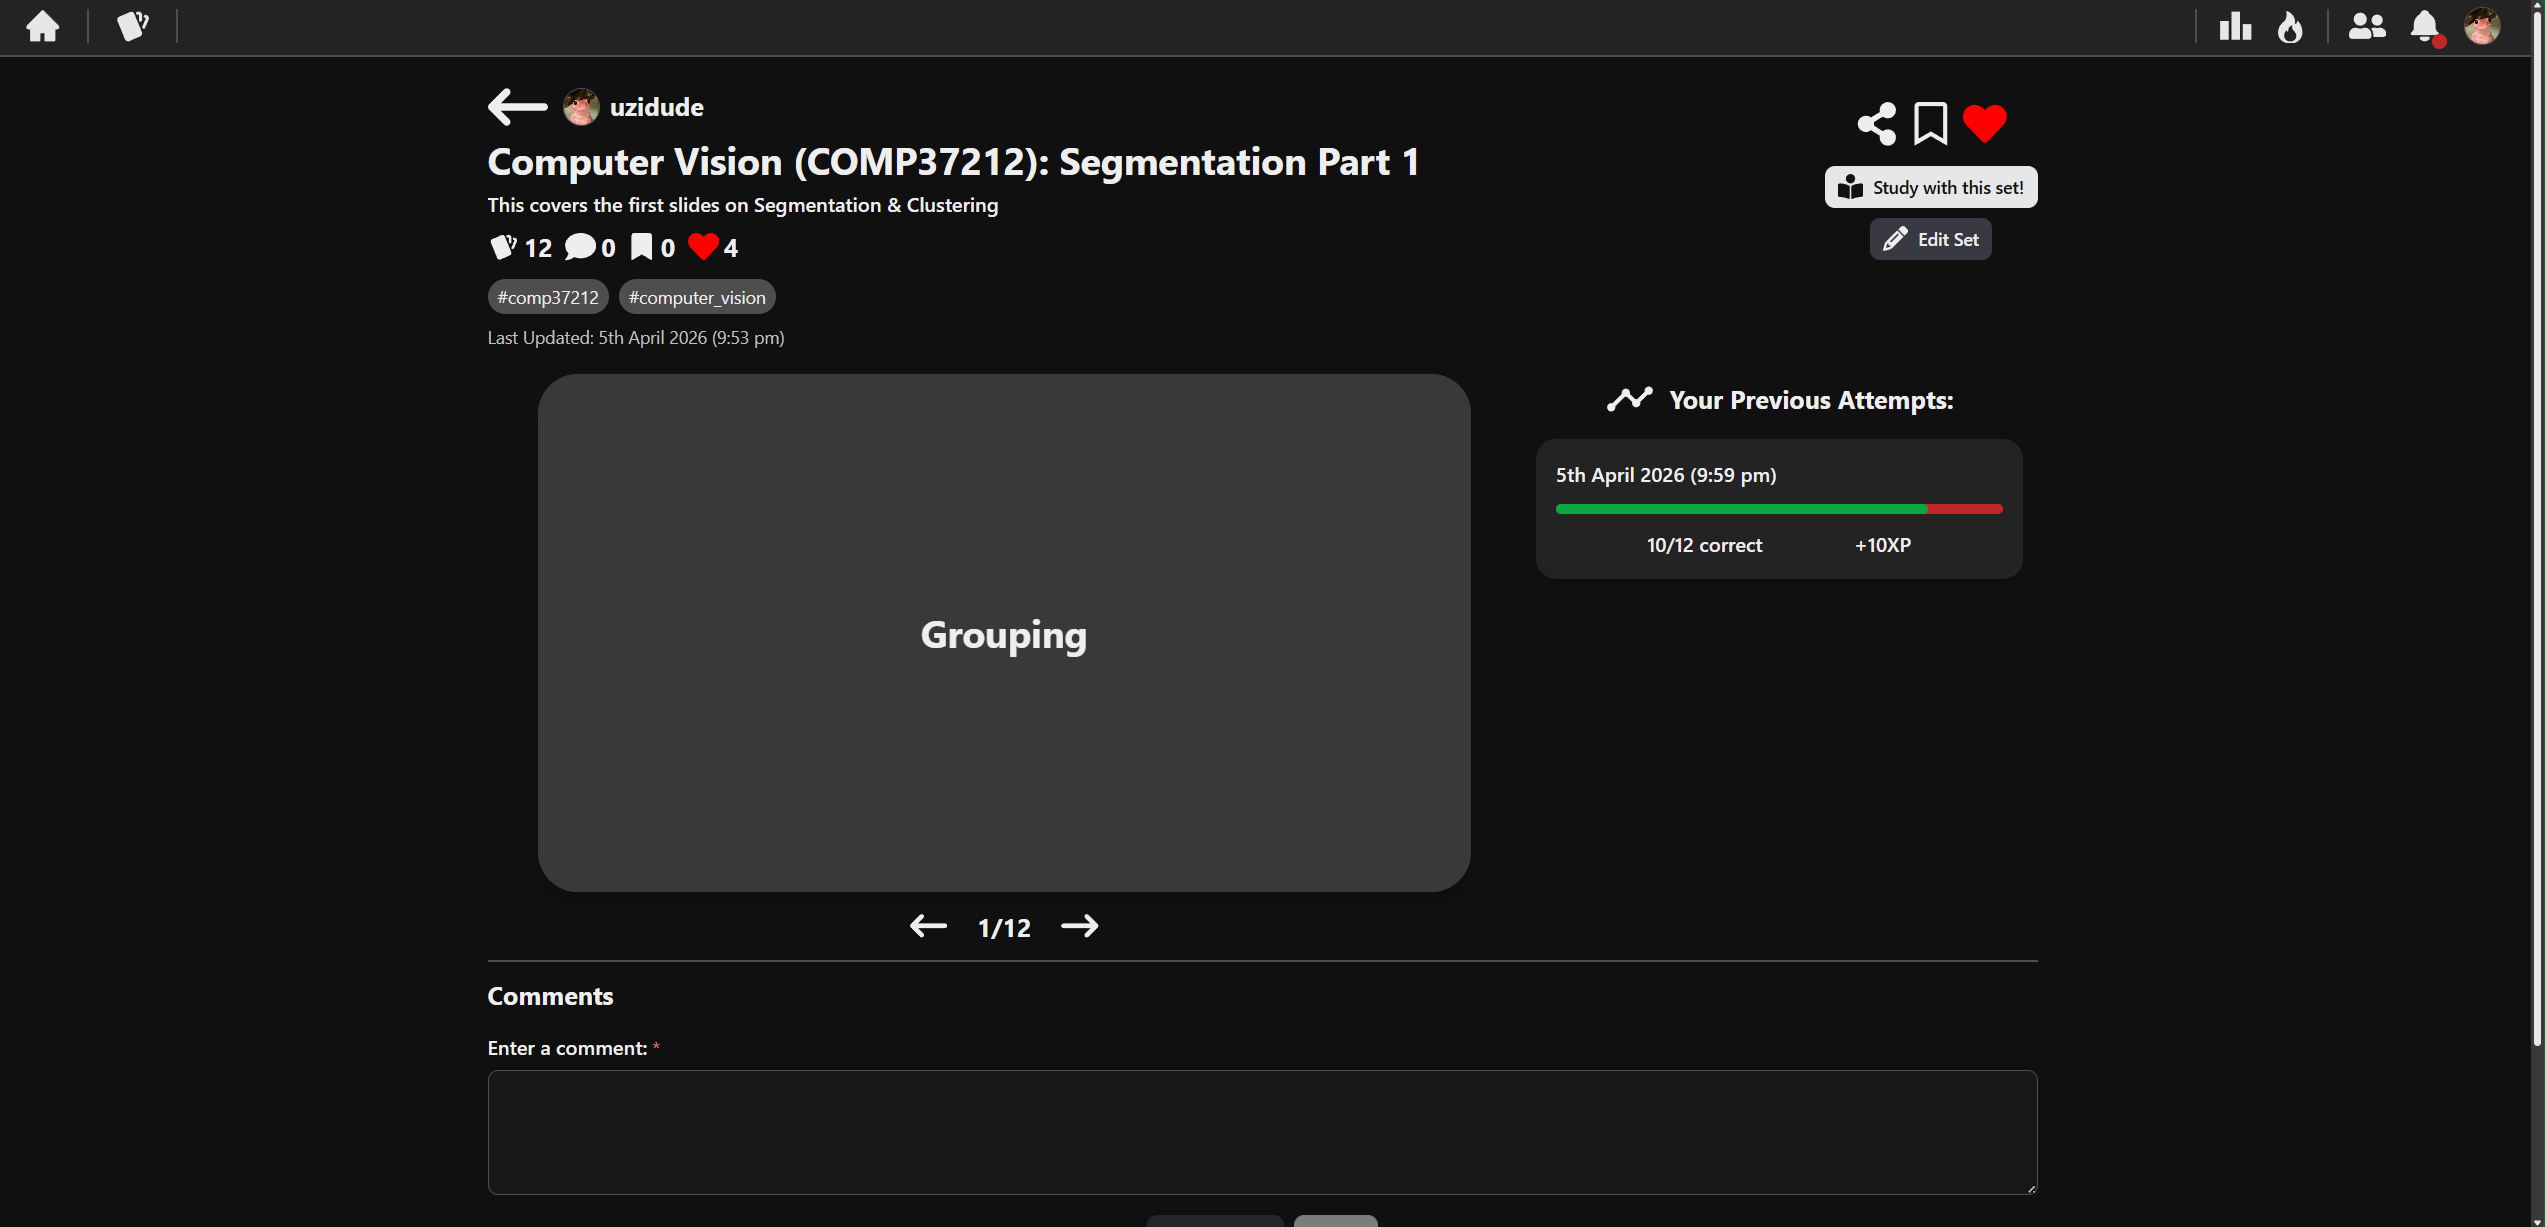
\includegraphics[width=\linewidth, keepaspectratio]{Implementation/Themes/Charcoal.png}
        \caption{Charcoal}
        \label{fig:charcoal}
    \end{subfigure}

    \vspace{0.5cm}
    
    \begin{subfigure}{0.9\textwidth}
        \centering
        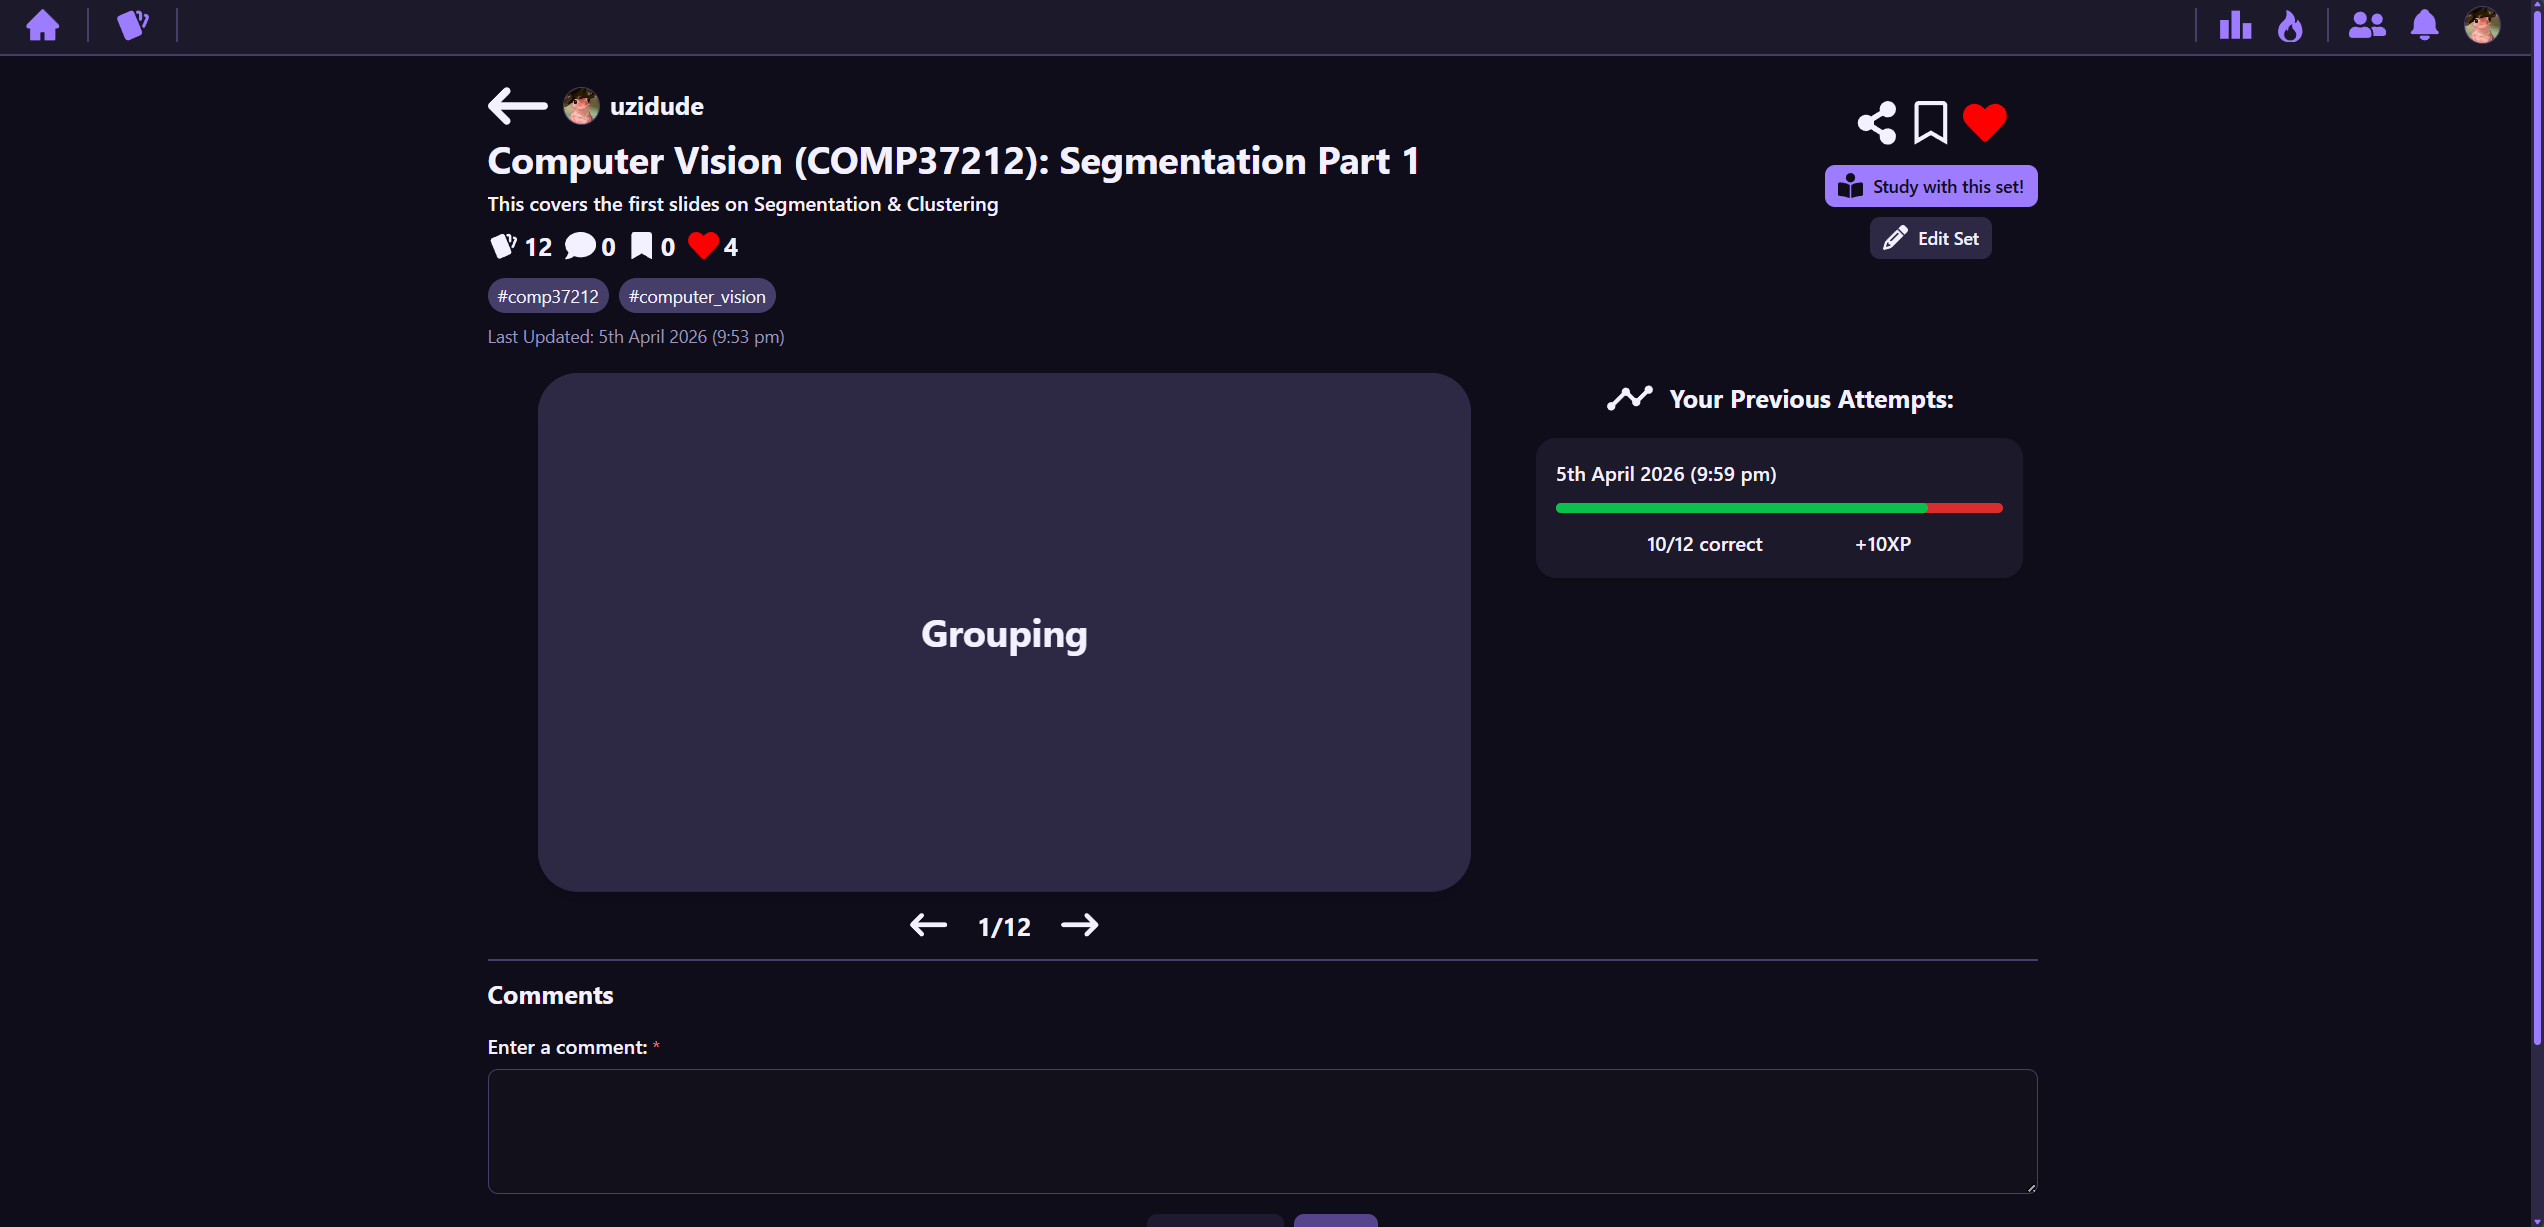
\includegraphics[width=\linewidth, keepaspectratio]{Implementation/Themes/MidnightPurple.png}
        \caption{Midnight Purple}
        \label{fig:midnightPurple}
    \end{subfigure}

    \vspace{0.5cm}
    
    \begin{subfigure}{0.9\textwidth}
        \centering
        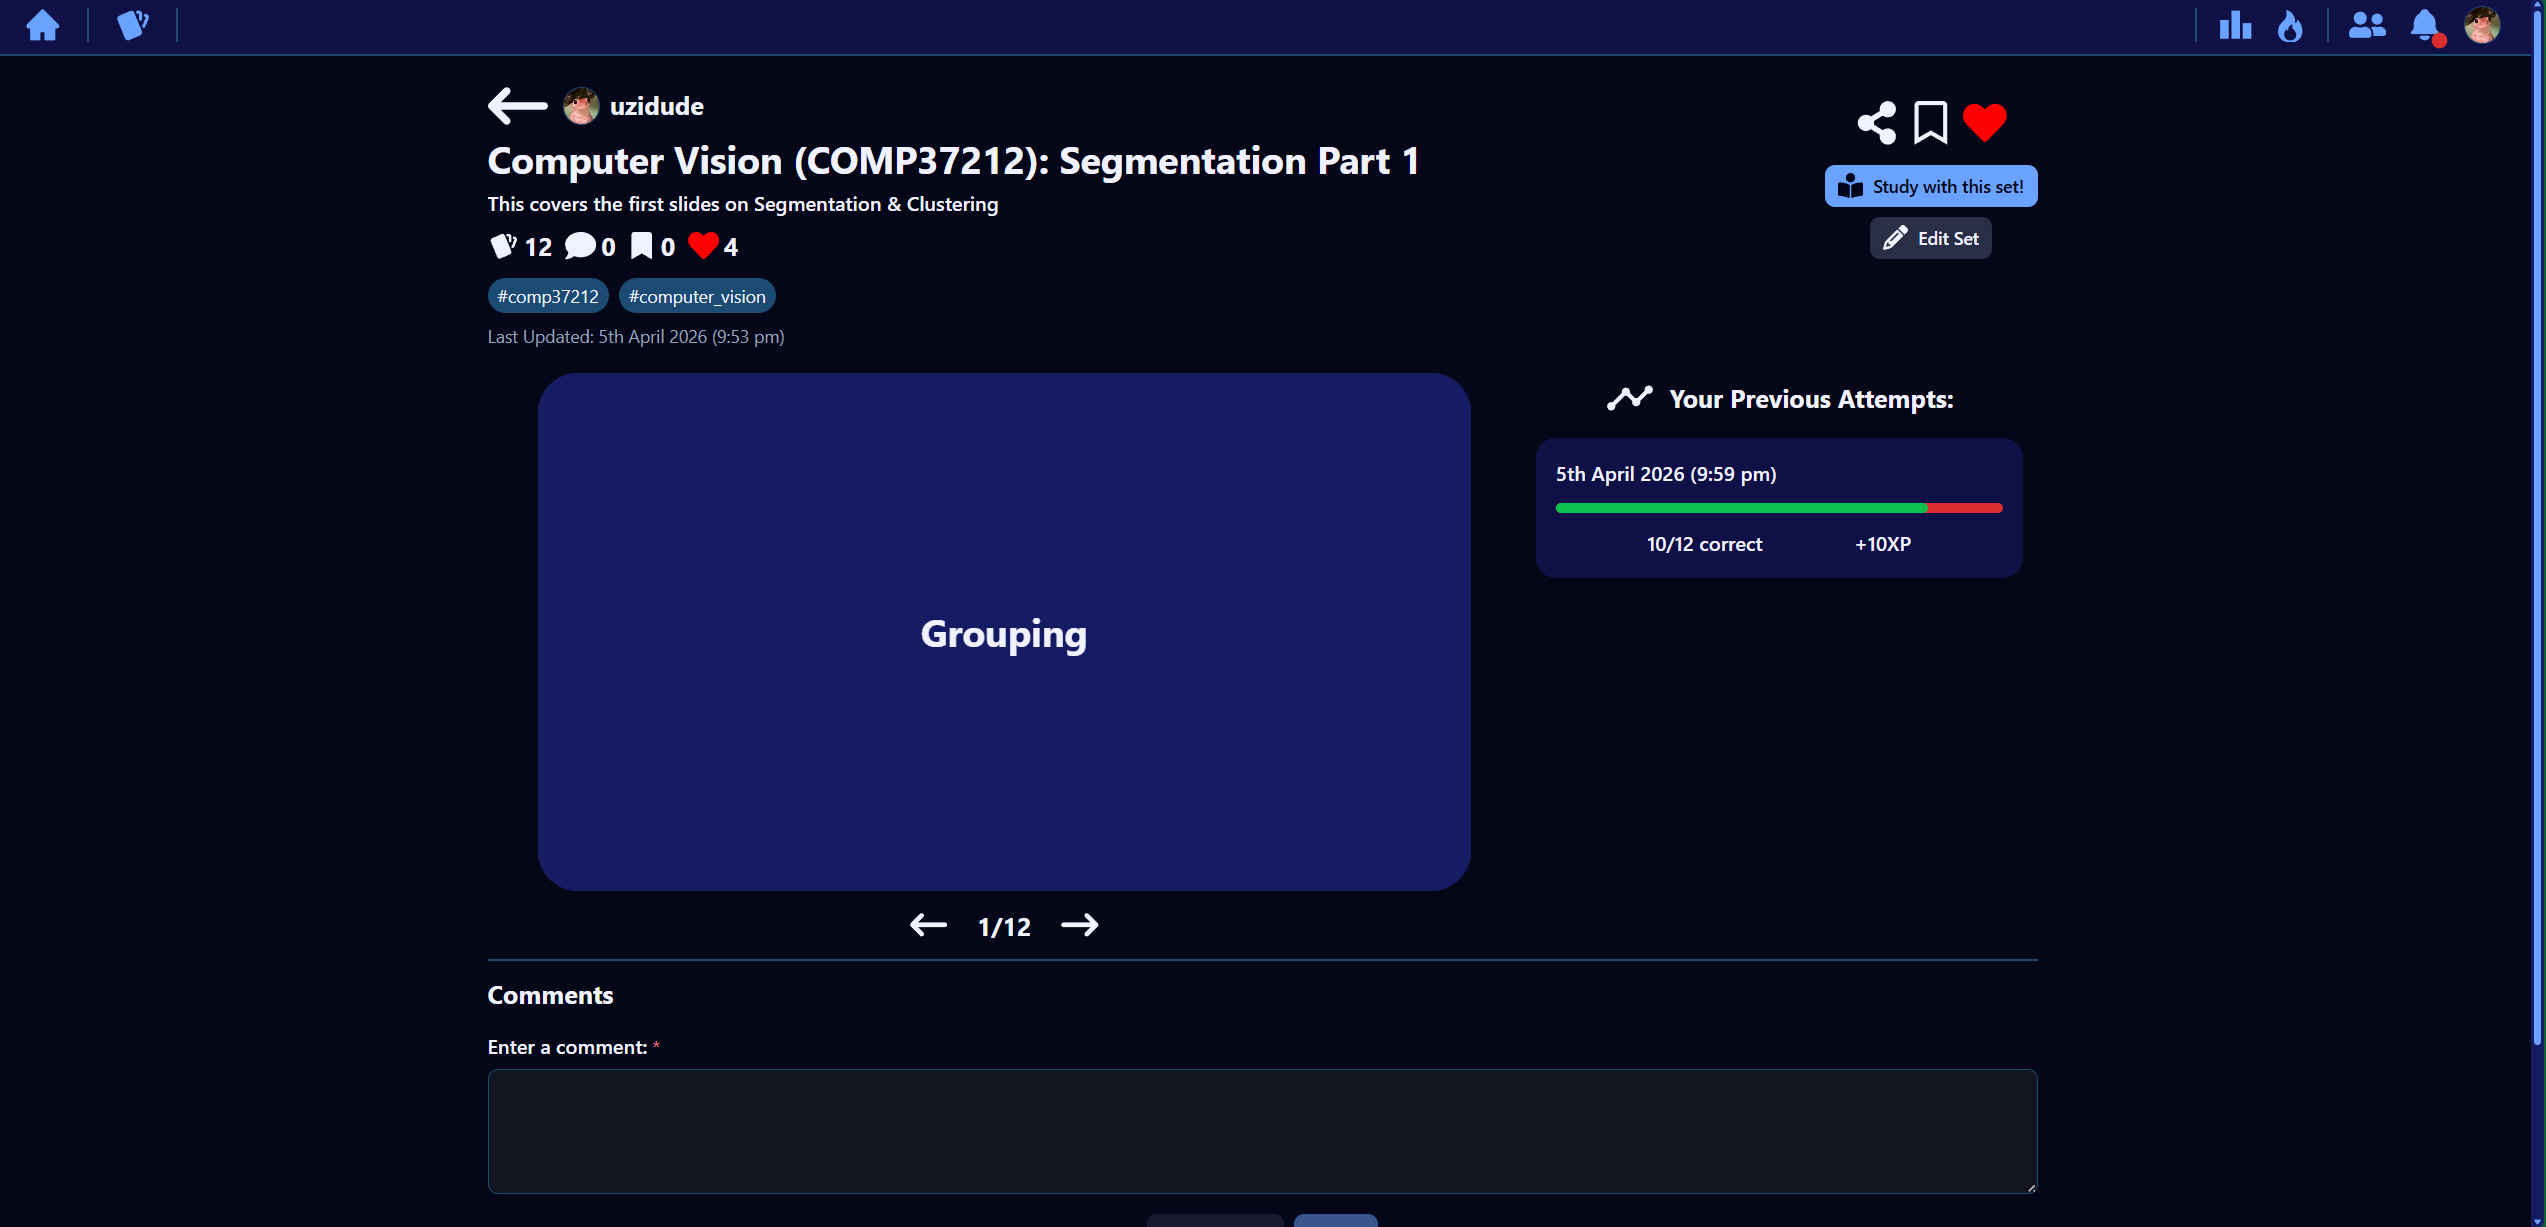
\includegraphics[width=\linewidth, keepaspectratio]{Implementation/Themes/OceanBlue.png}
        \caption{Ocean Blue}
        \label{fig:oceanBlue}
    \end{subfigure}
    \caption{A selection of the dark themes, shown on the flashcard set overview page}
    \label{fig:darkThemes}
\end{figure}

\subsection{Unlockable Achievements and Themes}

One of the standout 'gamification' features of ReviXion is the unlockable items.
ReviXion features achievements that users can strive for.
These achievements cover all aspects of the website, for example, engaging with the flashcard system, making friends, giving out likes, etc.
This is done with the intent that users will explore parts of the website they wouldn't usually engage with, without some reward or something to show for it.
In doing so, users can contribute to the growing library of flashcard sets, as well as make new friends in the community, adding to the social network aspect of the website.

All achievements have a clear unlock criteria, as well as an XP reward for unlocking the achievement.
Additionally, users will be made known of the percentage of users that have unlocked that achievement,
as this will encourage users to try to unlock the achievements that are considered 'rare'.

Furthermore, users can unlock more themes to customise with by completing similar tasks.
Instead of just gaining XP like with the achievements, this gives users something more tangible to work towards,
and should feel like more of a 'reward' to the user.

\begin{figure}[H]
    \centering

    \begin{subfigure}{0.48\textwidth}
        \centering
        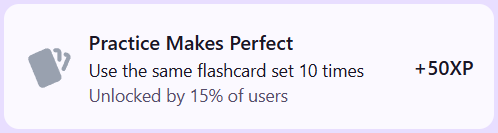
\includegraphics[width=\linewidth, keepaspectratio]{Implementation/Achievements/LockedAchievement1.png}
        \caption{A locked flashcard-based achievement}
        \label{fig:lockedAchievement1}
    \end{subfigure}
    \hfill
    \begin{subfigure}{0.48\textwidth}
        \centering
        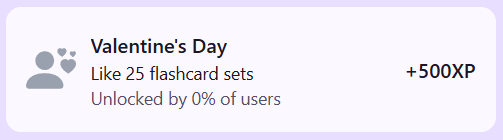
\includegraphics[width=\linewidth, keepaspectratio]{Implementation/Achievements/LockedAchievement2.png}
        \caption{A locked like-based achievement}
        \label{fig:lockedAchievement2}
    \end{subfigure}

    \vspace{0.5cm}

    \begin{subfigure}{0.48\textwidth}
        \centering
        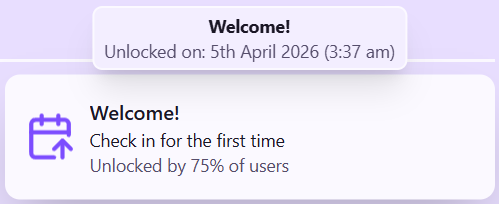
\includegraphics[width=\linewidth, keepaspectratio]{Implementation/Achievements/UnlockedAchievement1.png}
        \caption{An unlocked check-in-based achievement}
        \label{fig:unlockedAchievement1}
    \end{subfigure}
    \hfill
    \begin{subfigure}{0.48\textwidth}
        \centering
        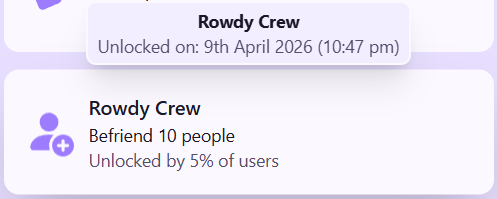
\includegraphics[width=\linewidth, keepaspectratio]{Implementation/Achievements/UnlockedAchievement2.png}
        \caption{An unlocked friend-based achievement}
        \label{fig:unlockedAchievement2}
    \end{subfigure}

    \caption{The different types of achievements users can unlock. Each achievement shows its unlock criteria, its XP (if locked), as well as the percentage of users who have earned that achievement.}
    \label{fig:achievements}
\end{figure}

\begin{figure}[H]
    \centering
    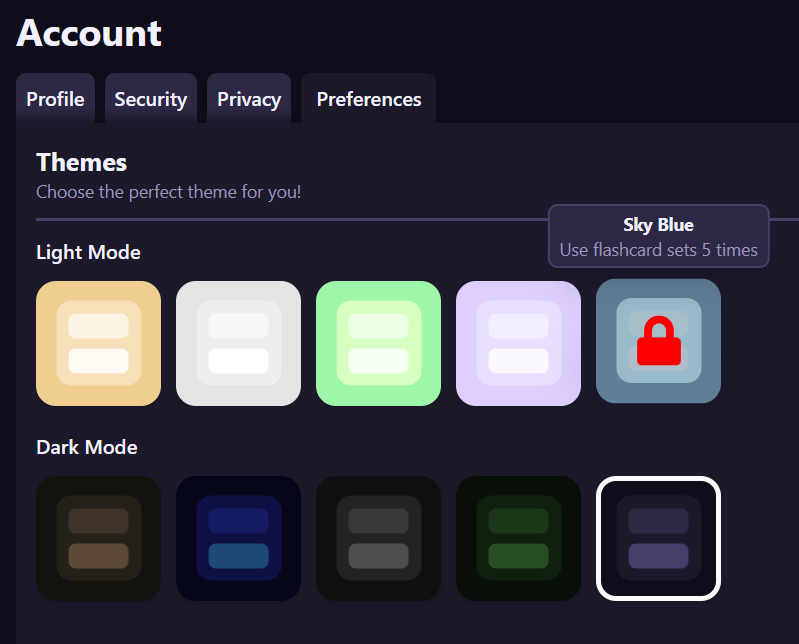
\includegraphics[width=0.8\linewidth]{Implementation/Themes/Themes.png}
    \caption{Available themes, some of which first need to be unlocked, indicated by their unlock criteria in the tooltip}
    \label{fig:themes}
\end{figure}

\subsection{Creating and Discovering Flashcard Sets}

The main study tool for this version of ReviXion is flashcards.
Users are given the ability to create their own flashcard sets, with options to add tags, description and tailor visibility (public or private).
Editing flashcard sets is also possible if users wish to make changes to an existing set.

\begin{figure}[H]
    \centering
    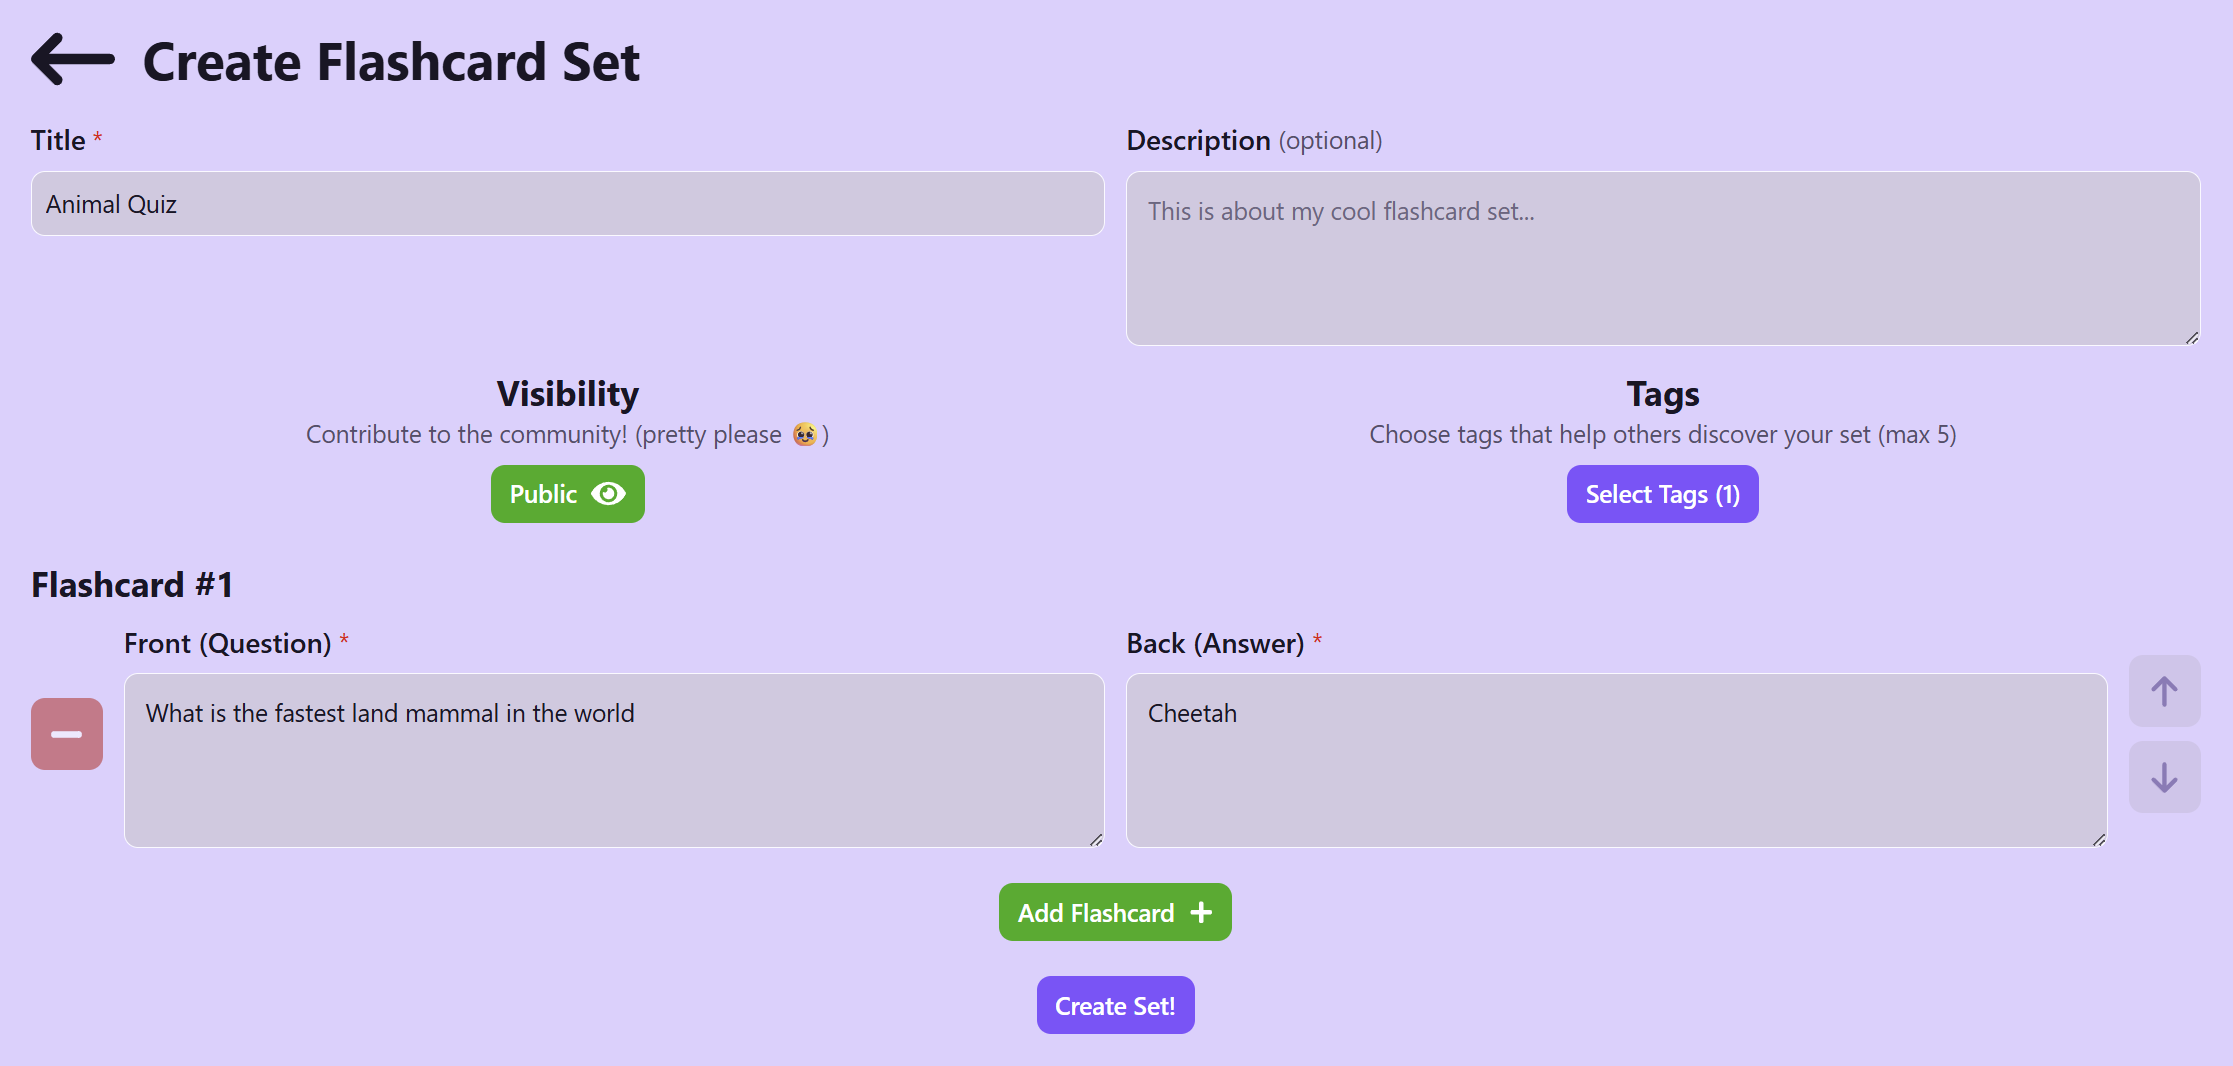
\includegraphics[width=\linewidth]{Implementation/Flashcards/CreateFlashcardSet.png}
    \caption{Create Flashcard Set page, also used for editing}
    \label{fig:createFlashcardSet}
\end{figure}

Flashcards have their own dedicated section of the website
where users can discover flashcard sets that have been created by other users.
Each set on this page has a concise overview that shows its title, description, tags, and more.
Users are given the ability to bookmark and like sets if they wish to save them or show appreciation.
These sets can be found through search, through associated tags,
or by filtering based on likes, bookmarks, or sets created by the user themselves.

\begin{figure}[H]
    \centering
    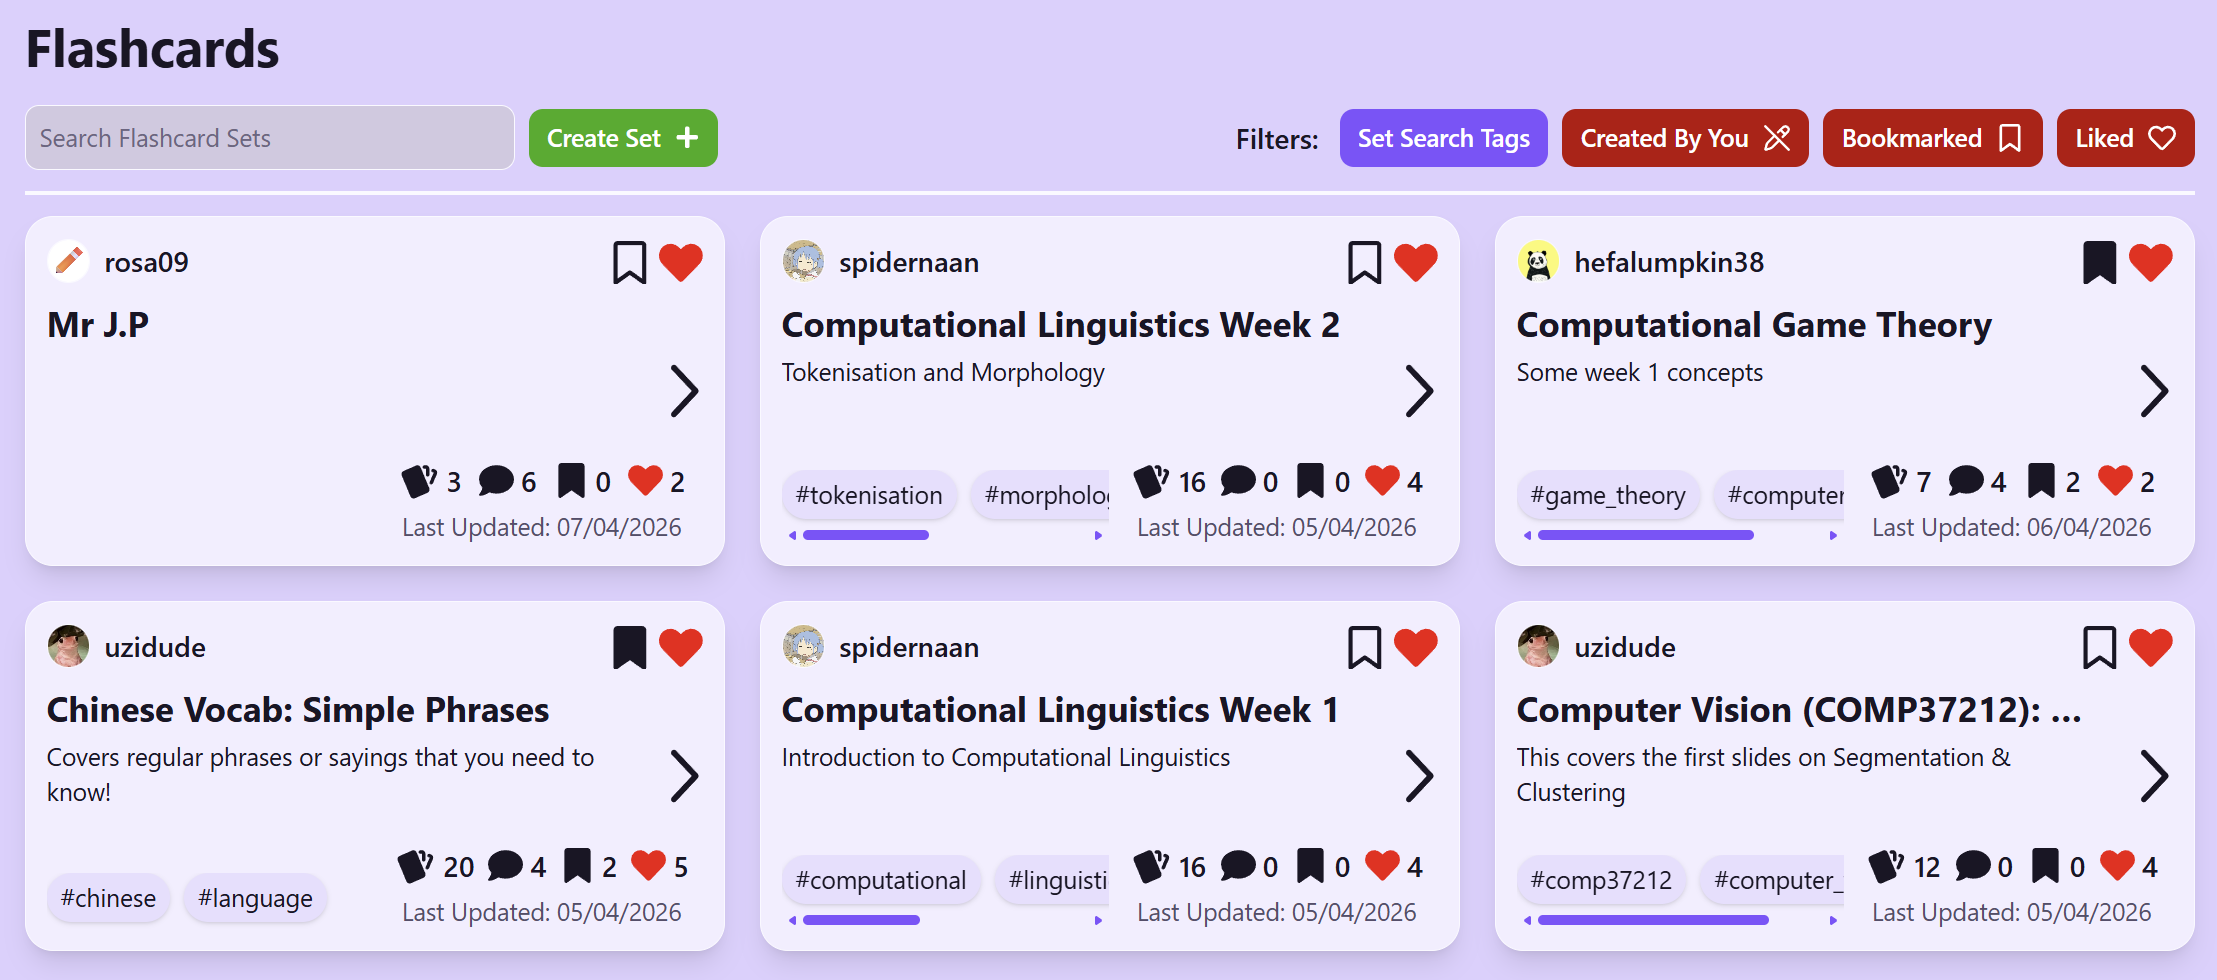
\includegraphics[width=\linewidth]{Implementation/Flashcards/FlashcardsPage.png}
    \caption{Flashcard Discovery Page, including search and filters}
    \label{fig:flashcardsPage}
\end{figure}

\subsection{Using Flashcard Sets}

When viewing a flashcard set, users get an expanded view,
showing key information about the set, as well as what flashcards are contained within the set.
Underneath each set, users are given the ability to comment,
which allows natural discussions to take place concerning the flashcards.
This is especially useful to allow users to encourage learning
and constructive criticism if mistakes are present or information is missing.
Comments can be replied to, which starts a chain of replies.
Comments can also be deleted if users wish to do so.

\begin{figure}[H]
    \centering
    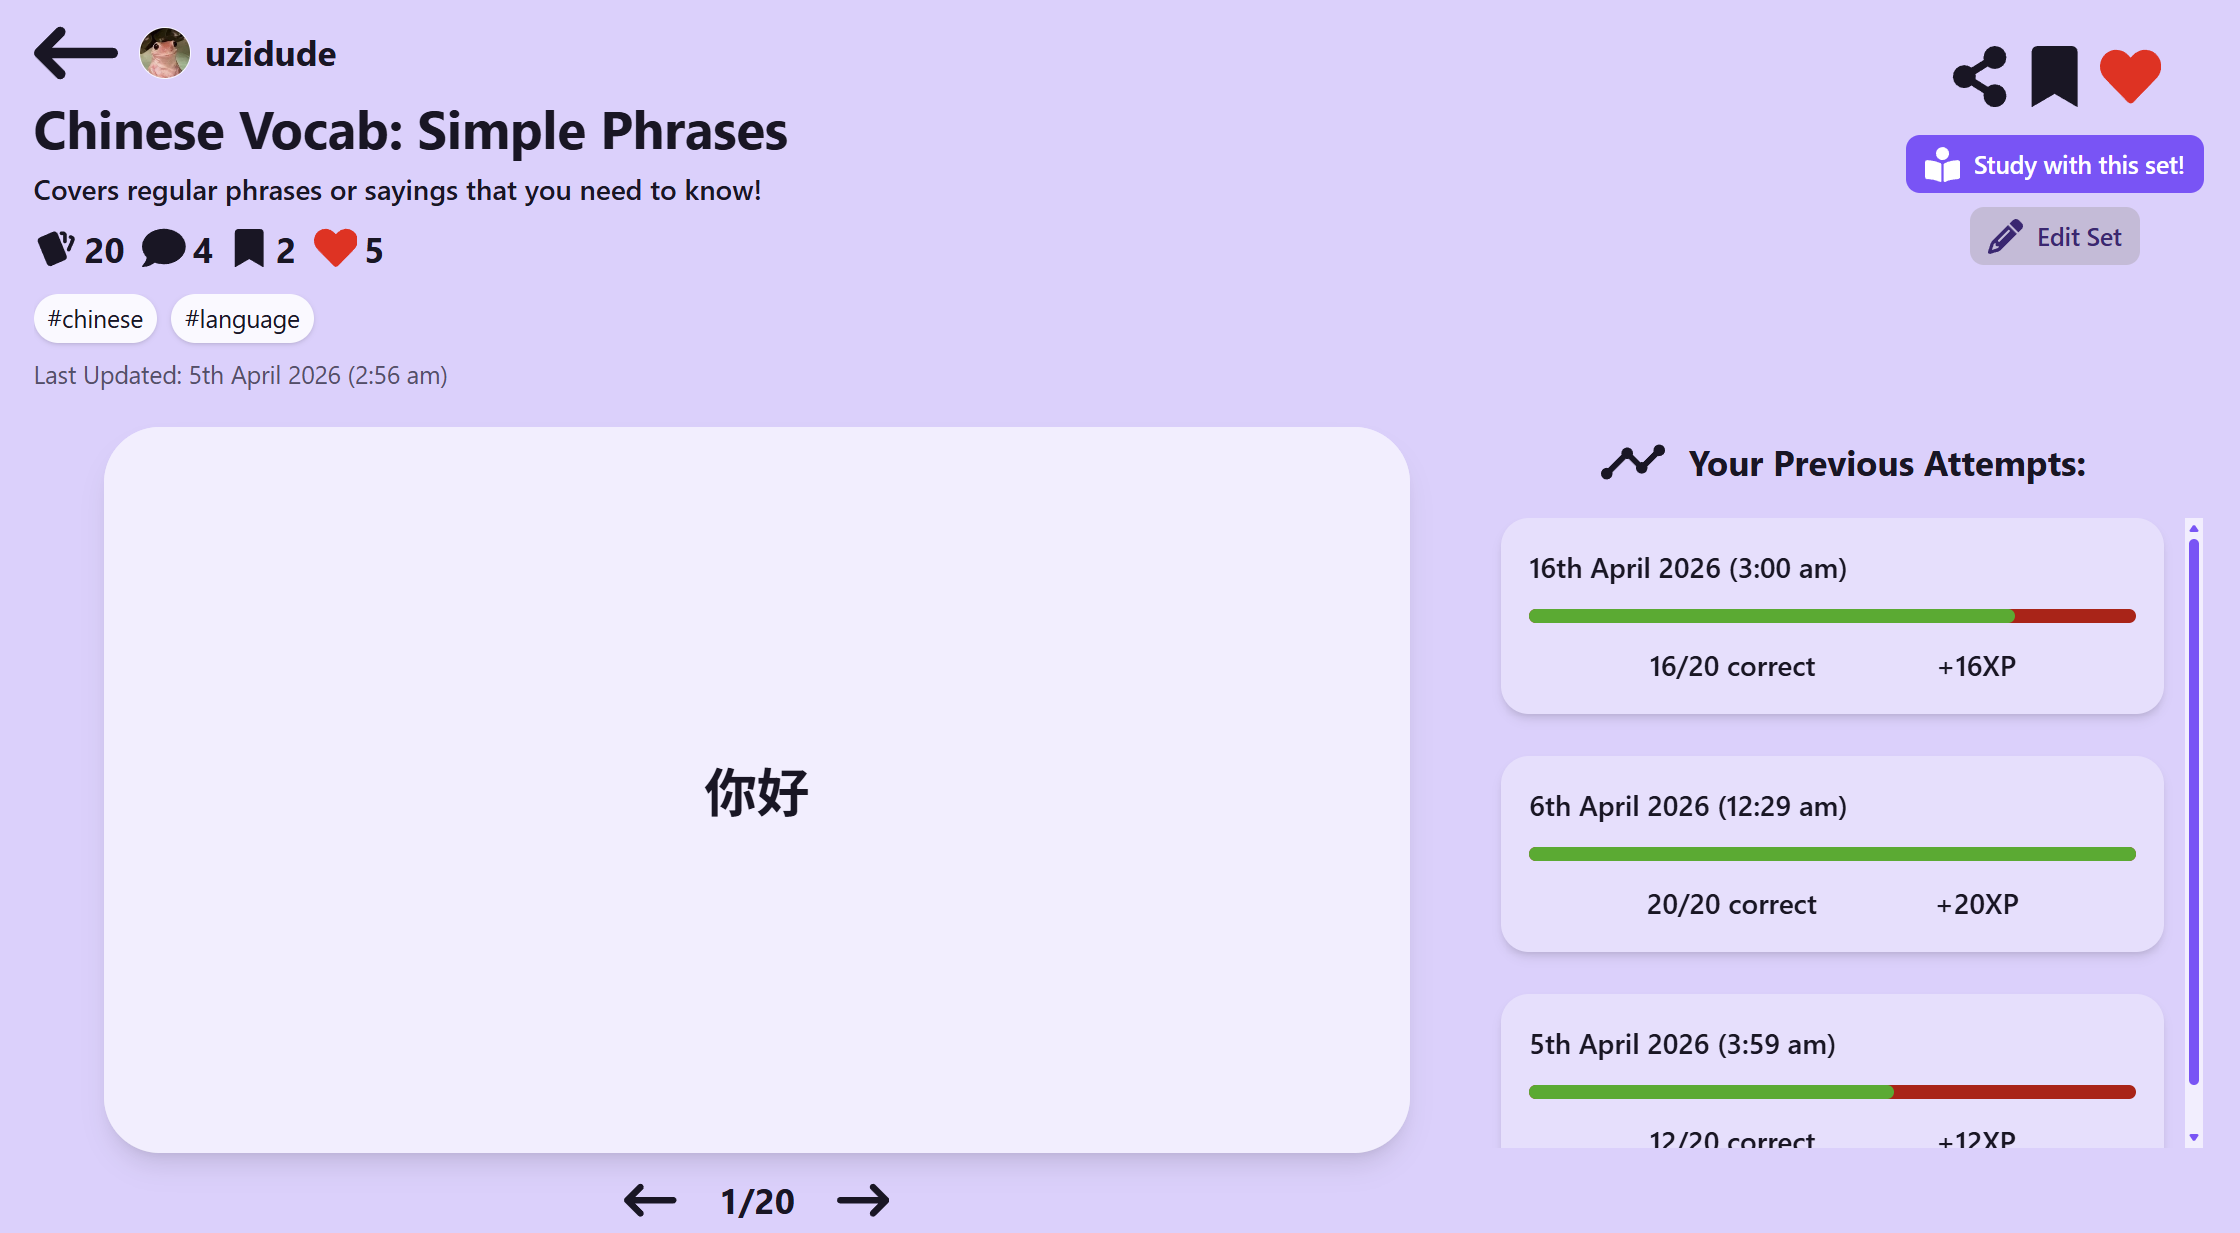
\includegraphics[width=\linewidth]{Implementation/Flashcards/FlashcardSetOverview.png}
    \caption{An example overview of a flashcard set}
    \label{fig:flashcardSetOverview}
\end{figure}

\begin{figure}[H]
    \centering
    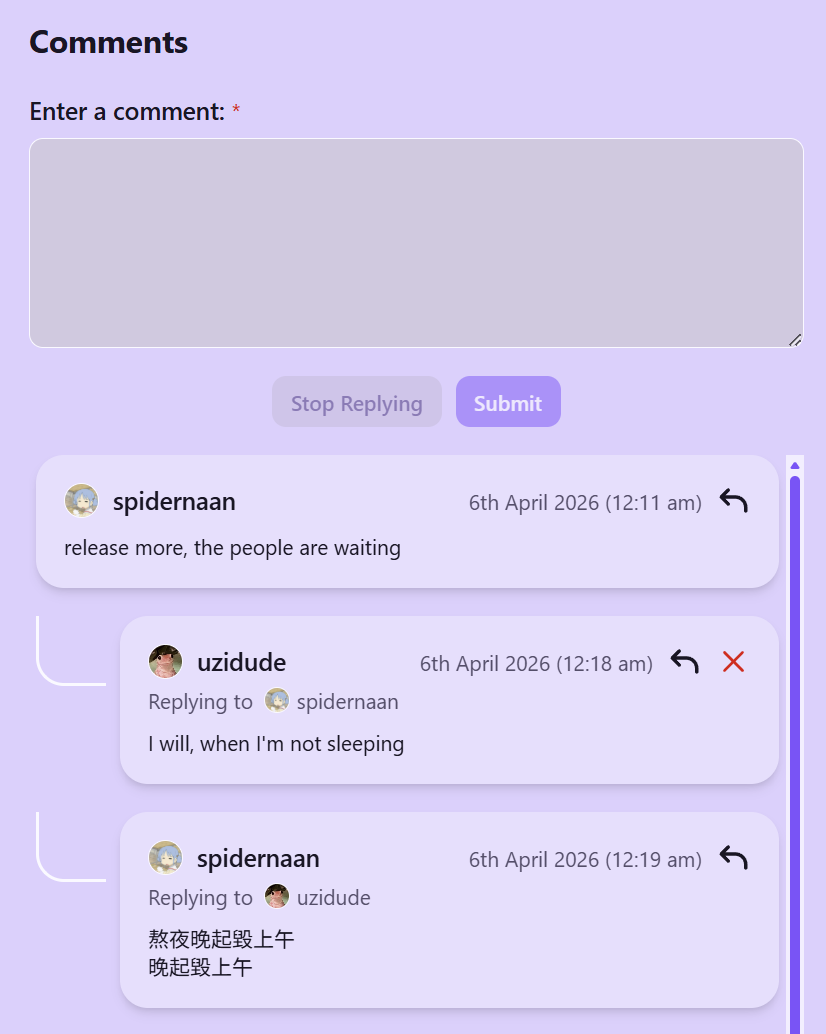
\includegraphics[width=0.5\linewidth]{Implementation/Flashcards/CommentSection.png}
    \caption{An example comment section of a flashcard set}
    \label{fig:commentSection}
\end{figure}

To use a flashcard set, users can click the 'Study Mode' button,
which puts them into a more minimal, focused view with just the flashcards and buttons to mark as correct or incorrect.
The flashcards can be shuffled to increase the difficulty, and users can undo their progress in case of misinputs.
For users on desktop, they are also given the option to use their keyboard to control the interface, which may be more efficient in some cases.

\begin{figure}[H]
    \centering
    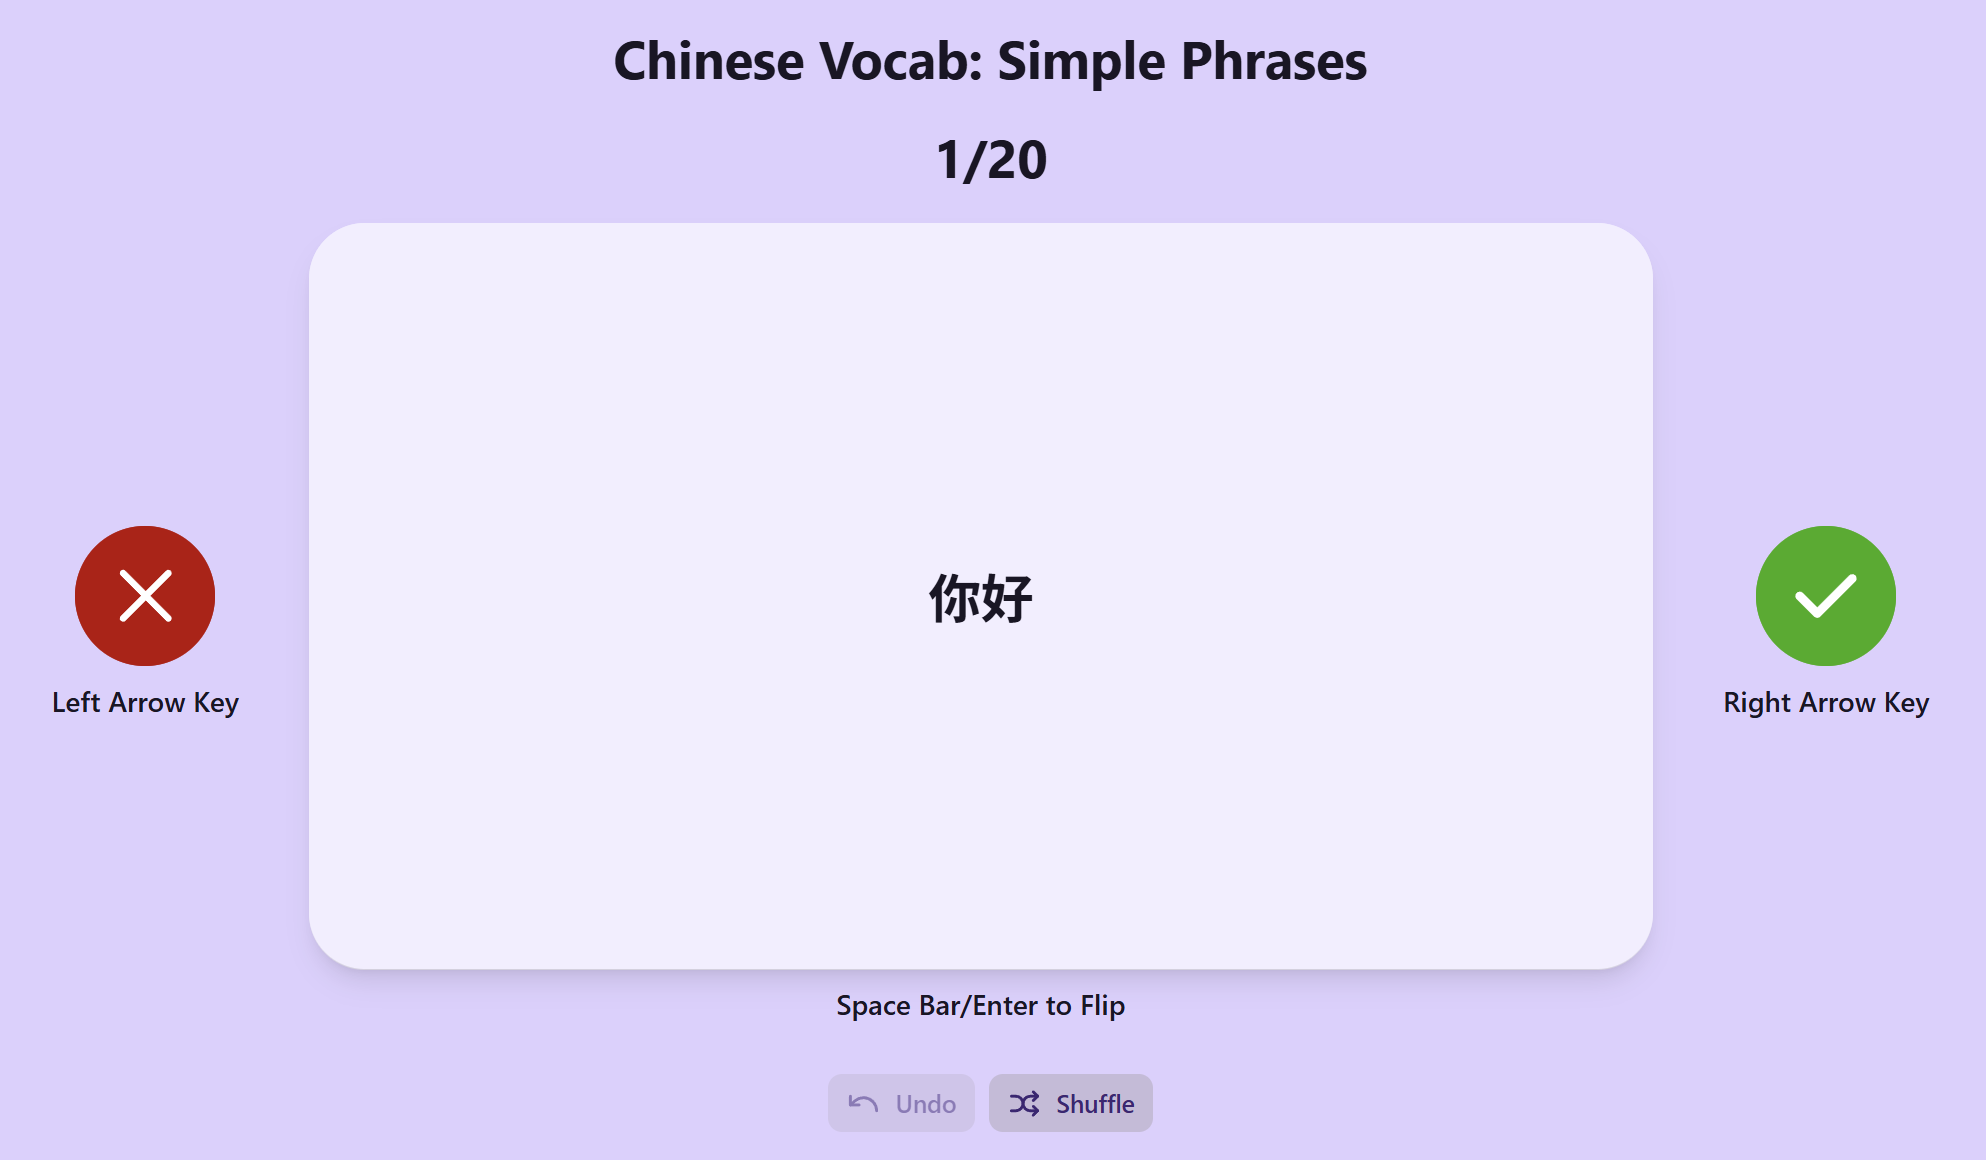
\includegraphics[width=0.8\linewidth]{Implementation/Flashcards/StudyMode.png}
    \caption{Using a flashcard set in Study Mode}
    \label{fig:studyMode}
\end{figure}

Once completing a flashcard set, a certain amount of XP is rewarded based on the ratio of correct to incorrect answers.
Their attempt is also recorded, and can be viewed on the overview page,
alongside a bar indicating how many flashcards were answered correctly.
This gives users instant feedback on whether they are improving based on their previous attempts,
and encourages spaced repetition if a user has not practiced with a certain set in a long time.

\begin{figure}[H]
    \centering
    \begin{minipage}{0.40\linewidth}
        \centering
        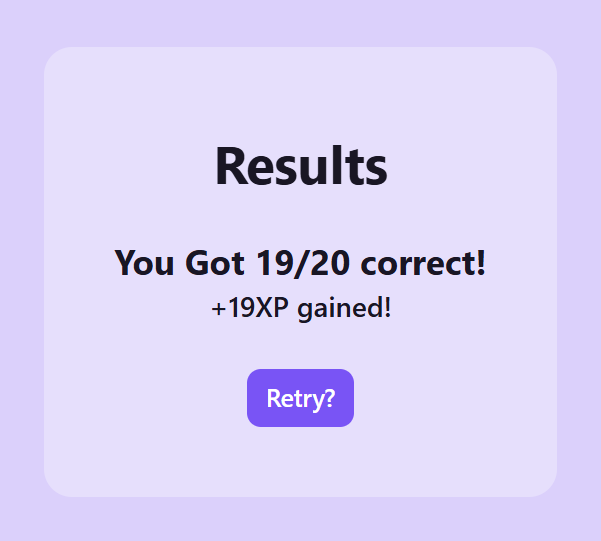
\includegraphics[width=0.8\linewidth]{Implementation/Flashcards/StudyModeResults.png}
        \caption{Results after using a flashcard set}
        \label{fig:studyModeResults}
    \end{minipage}
    \hfill
    \begin{minipage}{0.52\linewidth}
        \centering
        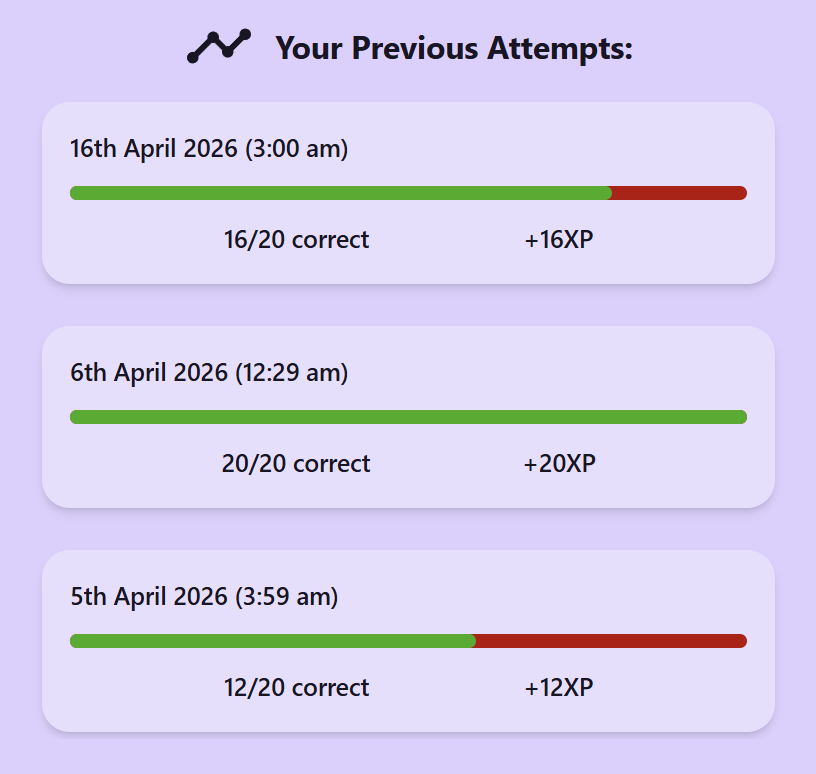
\includegraphics[width=\linewidth]{Implementation/Flashcards/History.png}
        \caption{History of your previous attempts for the flashcard set}
        \label{fig:history}
    \end{minipage}
\end{figure}

\subsection{Friends System}

One of ReviXion's core features is the friend system, which allows users to make friends and discover new people.
Users are given lots of opportunities to naturally discover new potential friends,
such as from the leaderboards (see Fig. \ref{fig:leaderboardsDaysStudied}), from flashcard set creators (see Fig. \ref{fig:flashcardsPage} and \ref{fig:flashcardSetOverview}),
or even comments (see Fig. \ref{fig:commentSection}).
Users have the option to add friends by viewing their profile, or by searching their username.

Additionally, users have the option to ignore friend requests, which places the request in an ignored section and does not inform the sender of the decision.
This can help to prevent spam or abuse of individuals. Users can also remove existing friends if they wish to do so.

\begin{figure}[H]
    \centering
    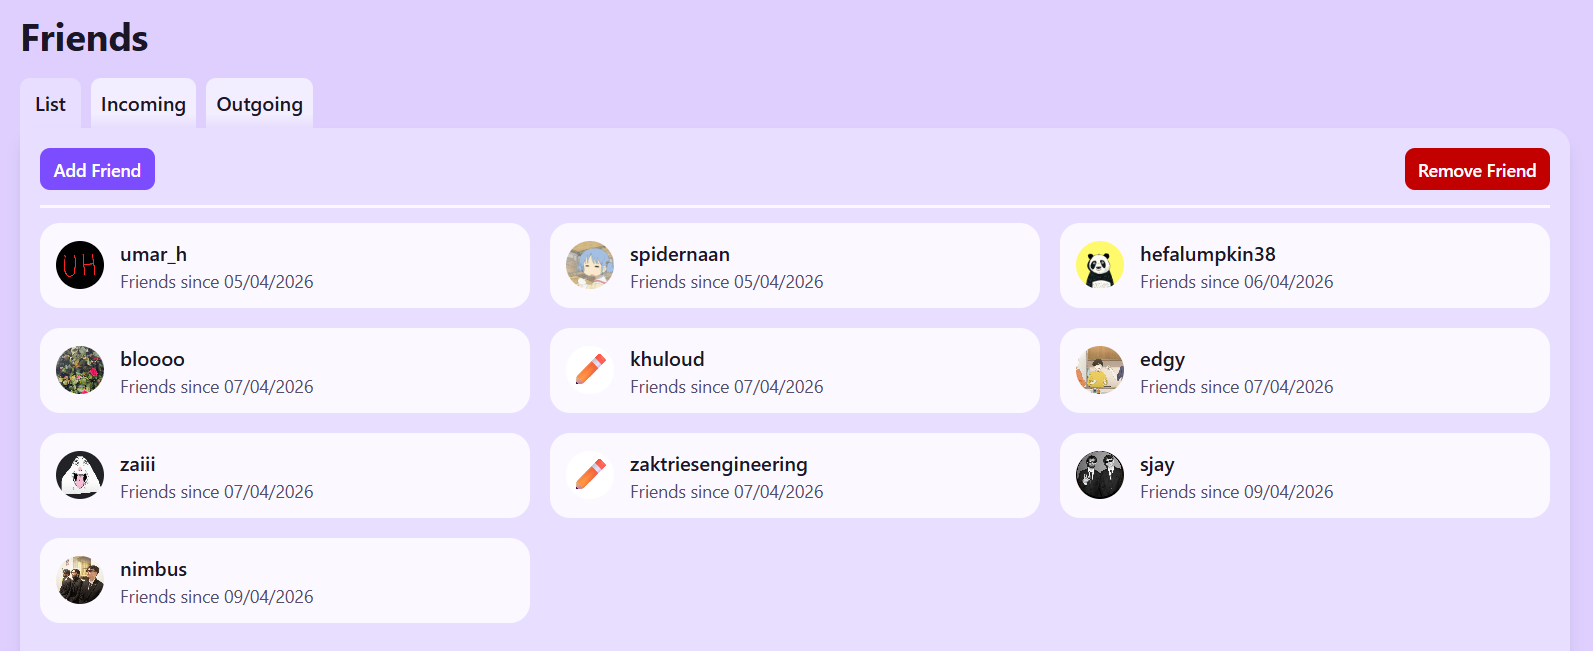
\includegraphics[width=\linewidth]{Implementation/Friends/FriendsList.png}
    \caption{Friends List section}
    \label{fig:friendsList}
\end{figure}

\begin{figure}[H]
    \centering
    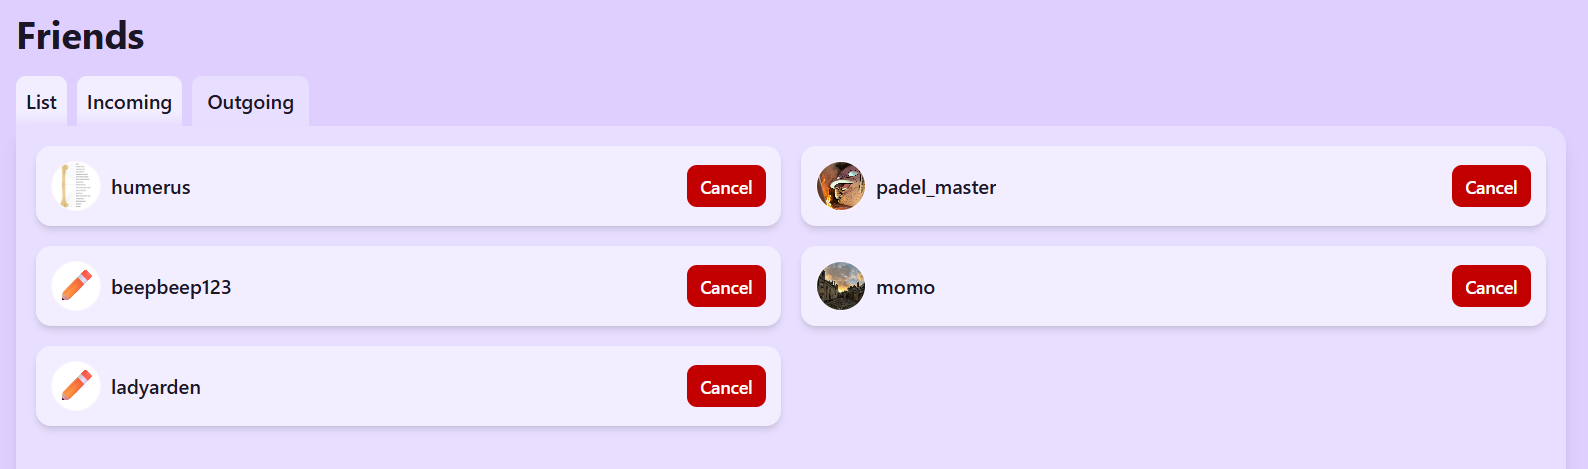
\includegraphics[width=\linewidth]{Implementation/Friends/FriendsOutgoing.png}
    \caption{Outgoing Friend Requests section}
    \label{fig:friendsOutgoing}
\end{figure}

\begin{figure}[H]
    \centering
    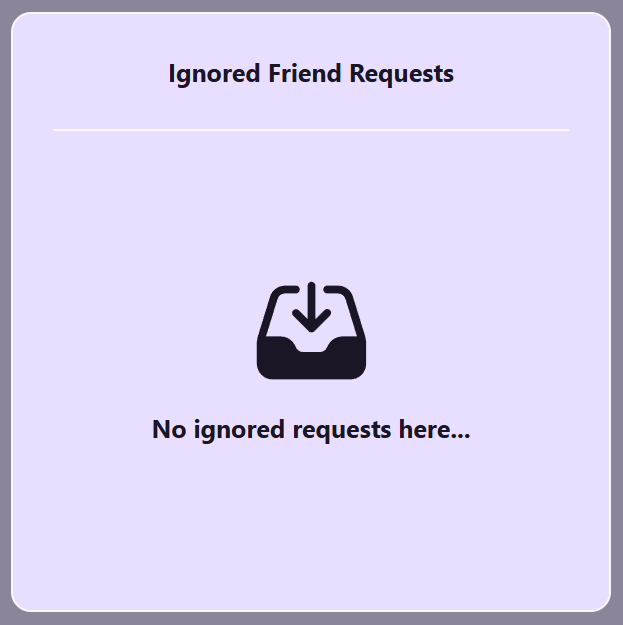
\includegraphics[width=0.4\linewidth]{Implementation/Friends/FriendsIgnored.png}
    \caption{Ignored Friend Requests pop-up}
    \label{fig:friendsIgnored}
\end{figure}

\subsection{Privacy Settings}

Users are given a range of privacy settings that allow them to tailor information about themselves that they would like to either be public, visible to friends, or private.
Such settings can change the visibility of their name, friends, level, or even their visibility on the leaderboards.

These privacy settings try to strike a balance between forcing the user to be too open or too closed off.
Some settings, such as their name, can be completely private as this is considered sensitive information.
However, other settings, such as the leaderboards, only have options for public and friends only,
which encourages users to engage with these aspects of the website, even if only with close friends.
As an example, looking at Fig. \ref{fig:leaderboardsDaysStudied},
we can see that some users have chosen not to show their level on the leaderboard.

Furthermore, when creating flashcards, users are given the option to make them public or private,
with a message to encourage users to create public flashcard sets in order to expand on the available sets and build the community.

\begin{figure}[H]
    \centering
    
\includegraphics[width=\linewidth]{Implementation/Privacy/PrivacySettings.png}
    \caption{Privacy settings, most of which can be toggled between 'Public', 'Friends Only' and 'Private'}
    \label{fig:privacySettings}
\end{figure}

\begin{figure}[H]
    \centering
    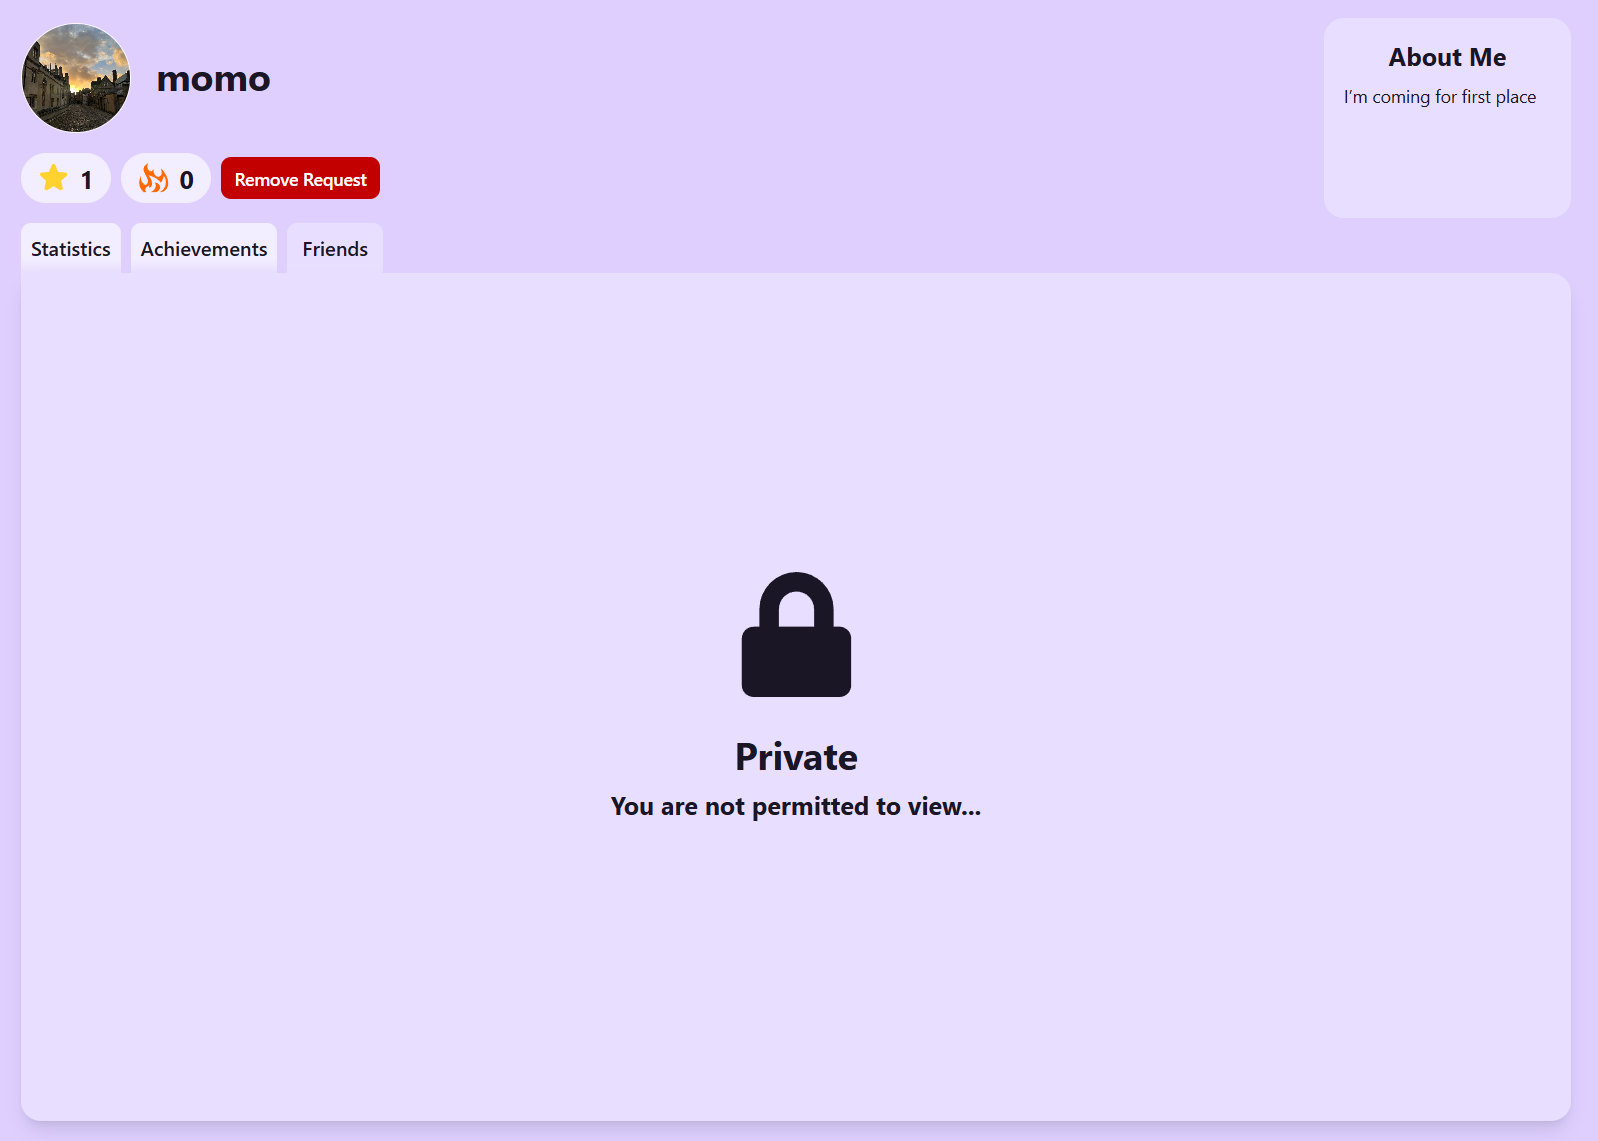
\includegraphics[width=0.8\linewidth]{Implementation/Privacy/PrivacyProfile.png}
    \caption{An example profile with hidden name and friends list}
    \label{fig:privacyProfile}
\end{figure}

\subsection{Notifications and Toasts}

ReviXion features real-time notifications and toast pop-ups for various events on the website.
Events include friend requests, unlocks, comments, likes, and so forth.
When an event triggers and sends a notification to a recipient, a respective toast will pop up to give the user immediate feedback of the event.
A ping will also remain above the notification icon until it has been acknowledged and read.

An early consideration was concerning receiving notifications for likes and bookmarks,
as users could mistakenly like a flashcard set, and take back the like a few seconds later.
In doing so, the recipient will have already been notified of the like.
The solution is to implement a buffer of one minute before sending these notifications to the recipient.
This gives the user time to act if they did make a mistake.

\begin{figure}[H]
    \centering
    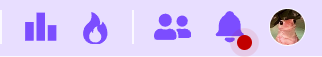
\includegraphics[width=0.5\linewidth]{Implementation/Notifications/NotificationPing.png}
    \caption{Ping notifying the user of unread notifications}
    \label{fig:notificationPing}
\end{figure}

\begin{figure}[H]
    \centering
    \begin{subfigure}{0.48\textwidth}
        \centering
        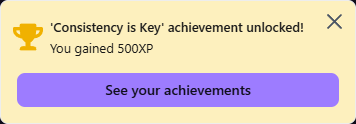
\includegraphics[width=\linewidth]{Implementation/Notifications/ToastAchievement.png}
        \caption{Achievement Toast}
        \label{fig:toastAchievement}
    \end{subfigure}
    \hfill
    \begin{subfigure}{0.48\textwidth}
        \centering
        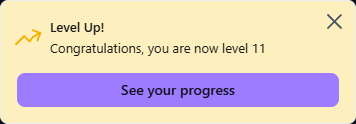
\includegraphics[width=\linewidth]{Implementation/Notifications/ToastLevel.png}
        \caption{Level Up Toast}
        \label{fig:toastLevel}
    \end{subfigure}
    
    \vspace{0.25cm}

    \begin{subfigure}{0.48\textwidth}
        \centering
        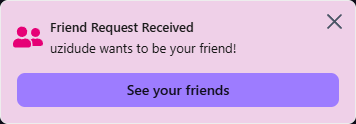
\includegraphics[width=\linewidth]{Implementation/Notifications/ToastFriend.png}
        \caption{Friend Toast}
        \label{fig:toastFriend}
    \end{subfigure}
    \hfill
    \begin{subfigure}{0.48\textwidth}
        \centering
        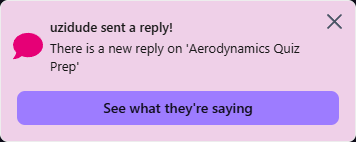
\includegraphics[width=\linewidth]{Implementation/Notifications/ToastComment.png}
        \caption{Comment Toast}
        \label{fig:toastComment}
    \end{subfigure}
    \caption{Toasts notifying the user in real-time of various events}
\end{figure}

Once the user has been notified through the toast, or log into the website and notice the ping,
they can access the notifications and are given a few actions to deal with them.
They can be redirected to the event that occurred, mark the notification as read/unread, or archive it.

\begin{figure}[H]
    \centering
    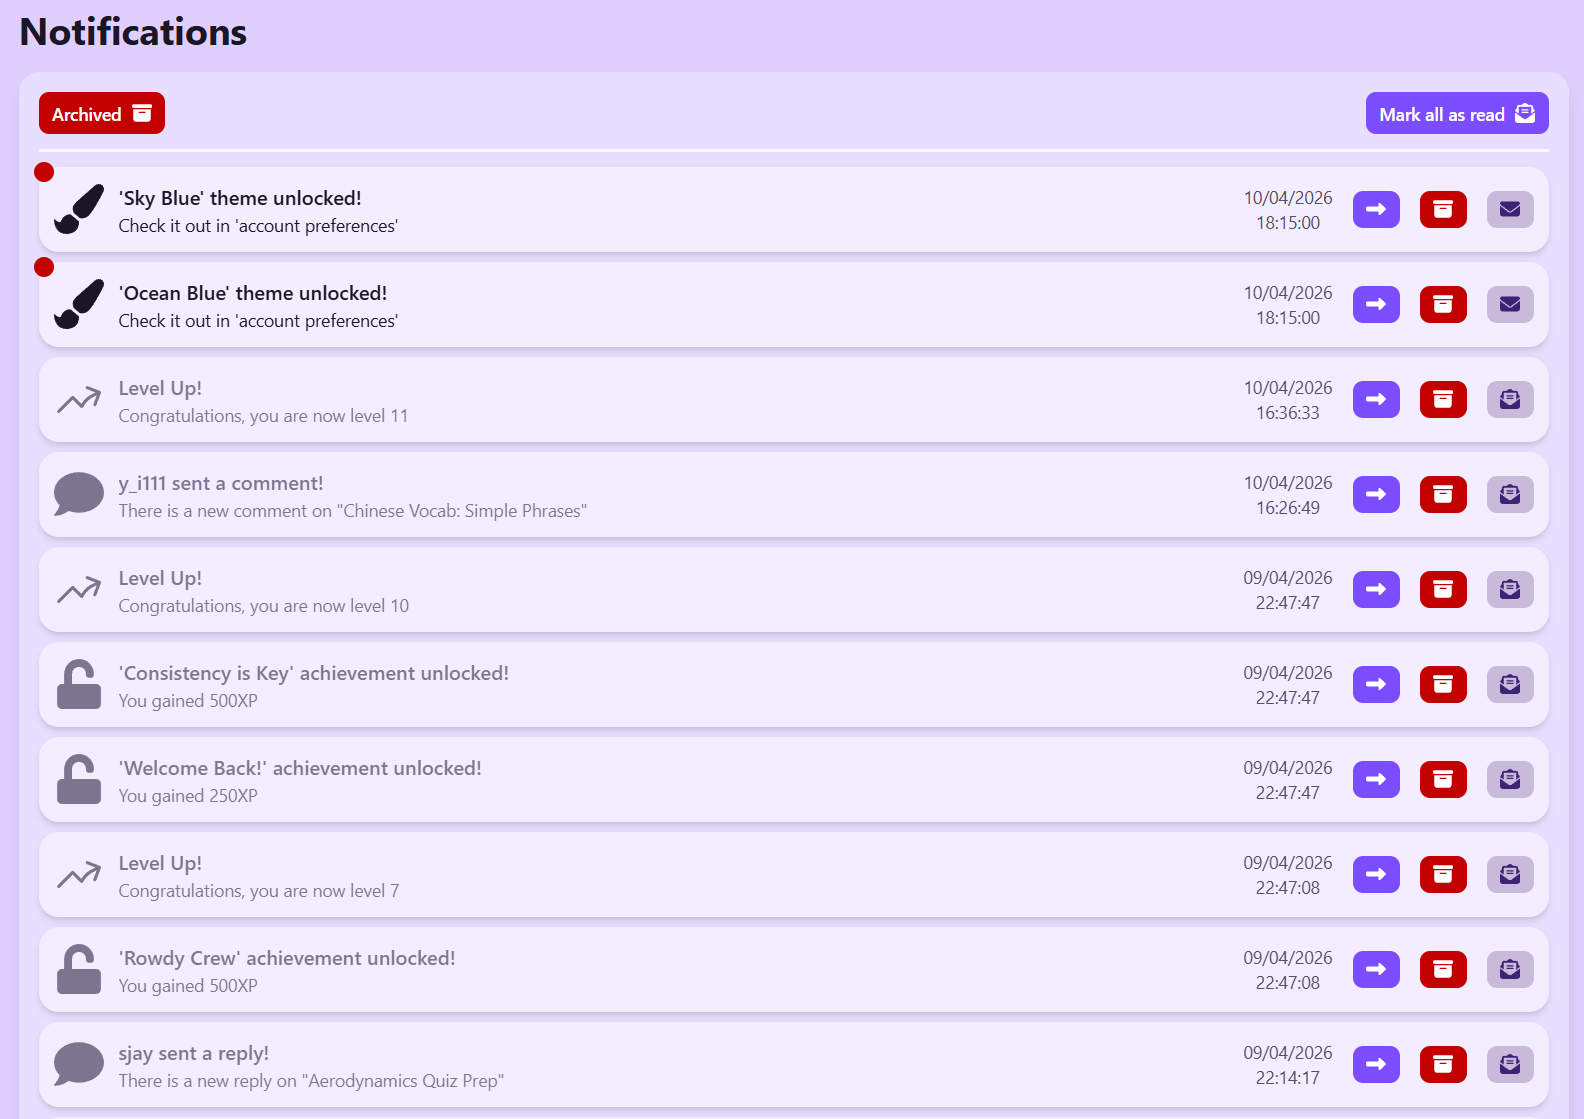
\includegraphics[width=\linewidth]{Implementation/Notifications/Notifications.png}
    \caption{Notifications page, showing the different kinds of notifications}
    \label{fig:notifications}
\end{figure}

\begin{figure}[H]
    \centering
    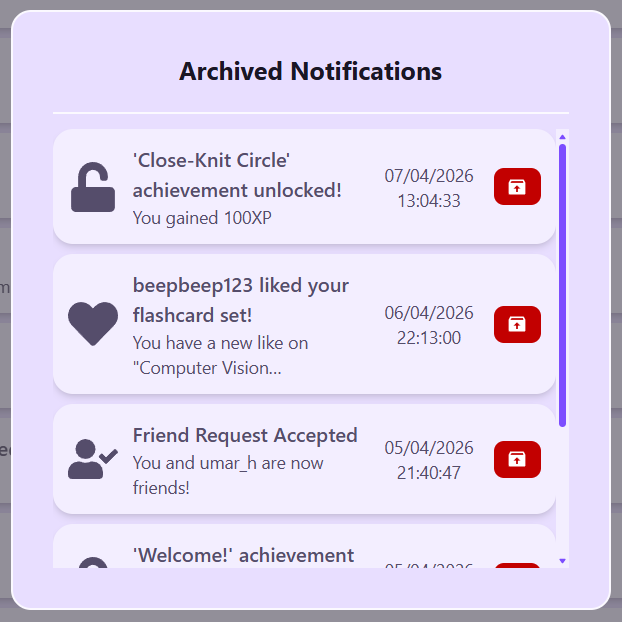
\includegraphics[width=0.6\linewidth]{Implementation/Notifications/NotificationsArchived.png}
    \caption{Archived notifications, which can be unarchived if needed}
    \label{fig:notificationsArchived}
\end{figure}

\subsection{Responsive Design}

ReviXion works on most devices with a browser, which includes desktop, mobile and tablet.
This is done through responsive design and Tailwind, which allows for different layouts based on the current width of the screen.
This is especially important for students who may wish to revise using their computer or laptop for long sessions in a stationary location,
or revise using their mobile phones on public transport.

\begin{figure}[H]
    \centering
    \begin{subfigure}{0.32\textwidth}
        \centering
        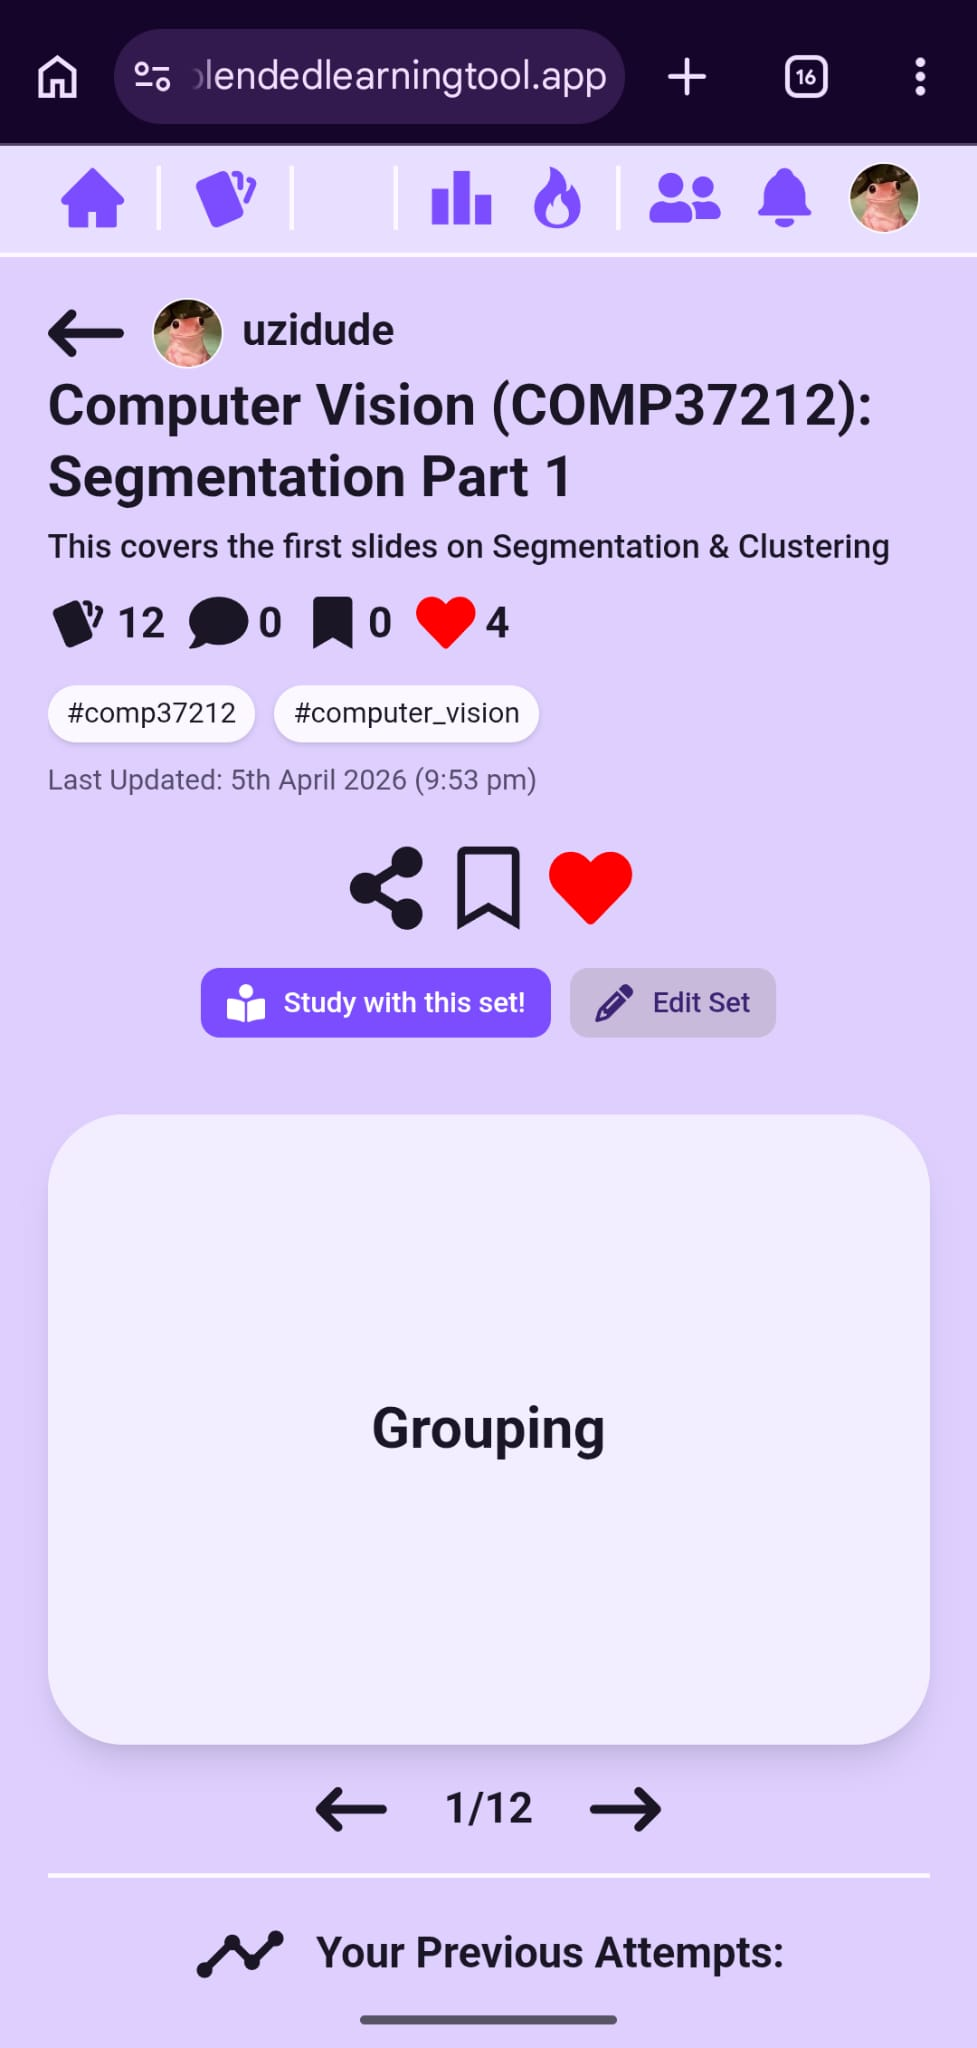
\includegraphics[width=0.9\linewidth, keepaspectratio]{Implementation/Mobile/MobileFlashcardSet.jpeg}
        \caption{Flashcard Set Page}
        \label{fig:mobileFlashcardSet}
    \end{subfigure}
    \hfill
    \begin{subfigure}{0.32\textwidth}
        \centering
        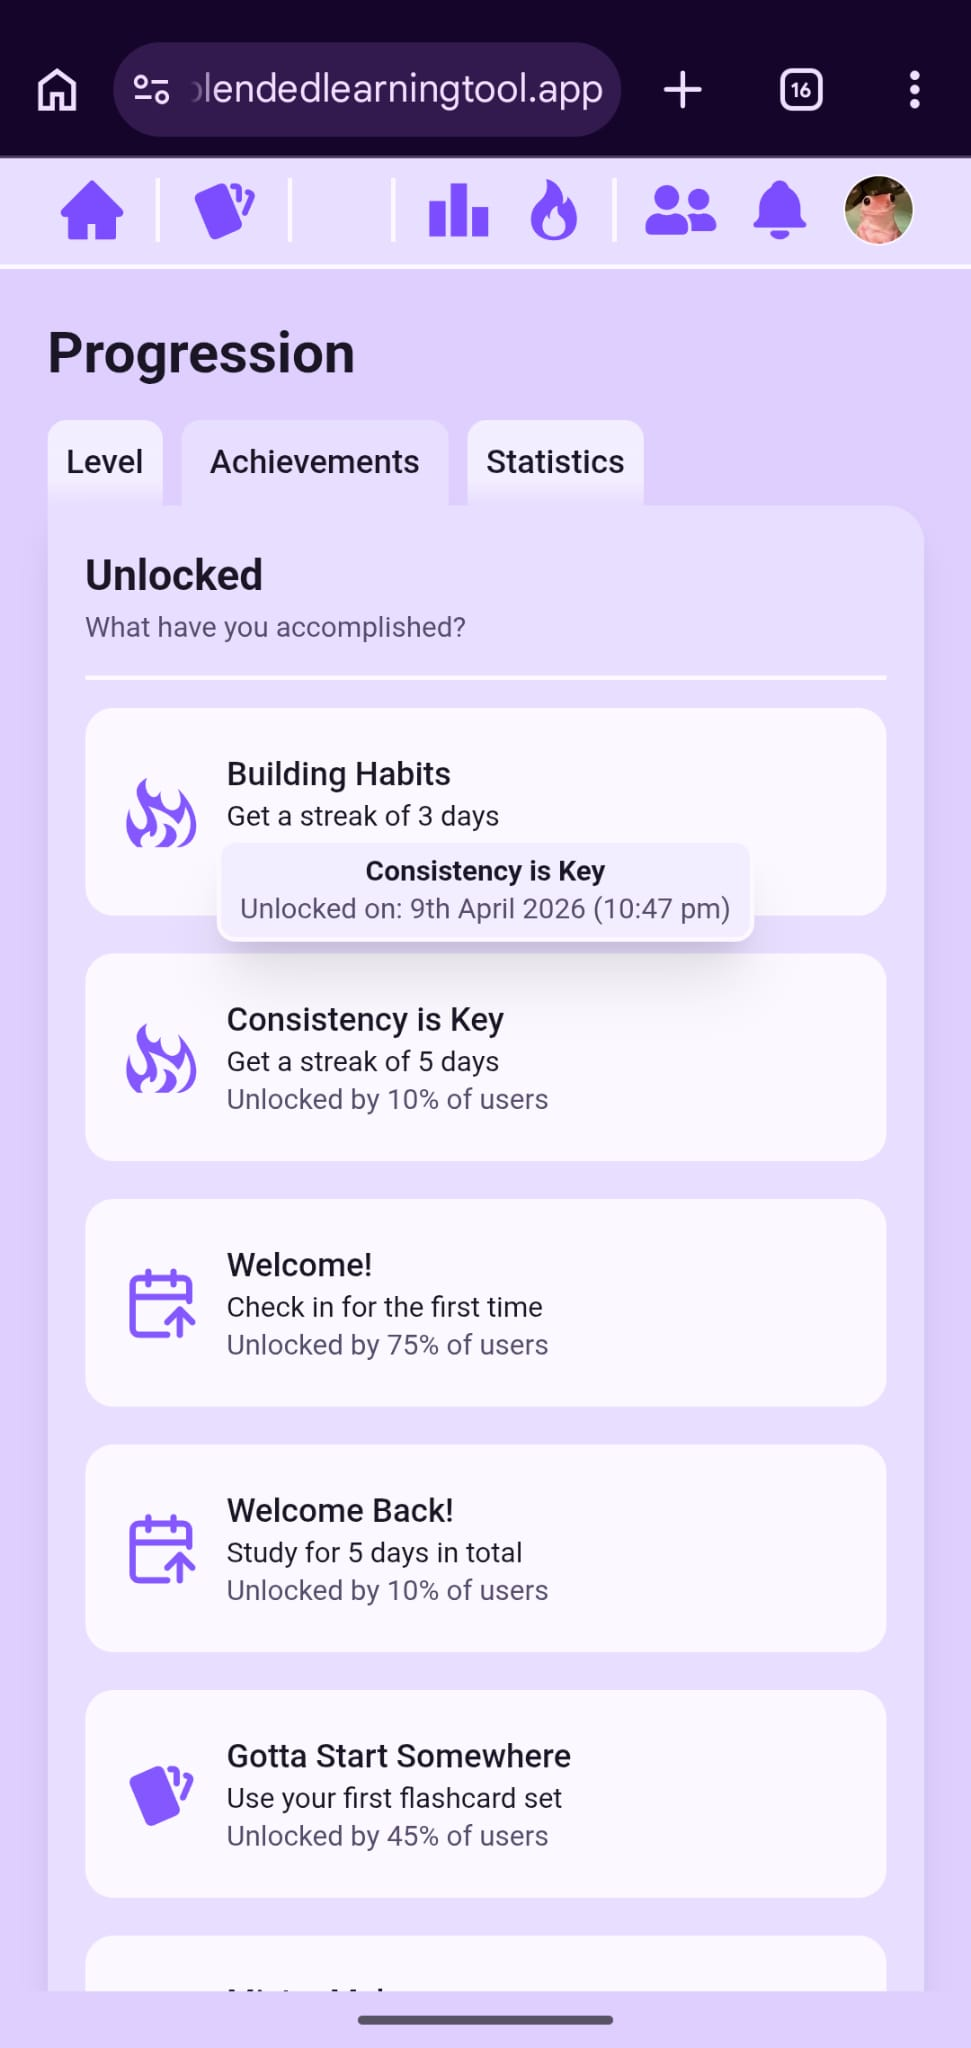
\includegraphics[width=0.9\linewidth, keepaspectratio]{Implementation/Mobile/MobileAchievements.jpeg}
        \caption{Achievements Page}
        \label{fig:mobileAchievements}
    \end{subfigure}
    \hfill
    \begin{subfigure}{0.32\textwidth}
        \centering
        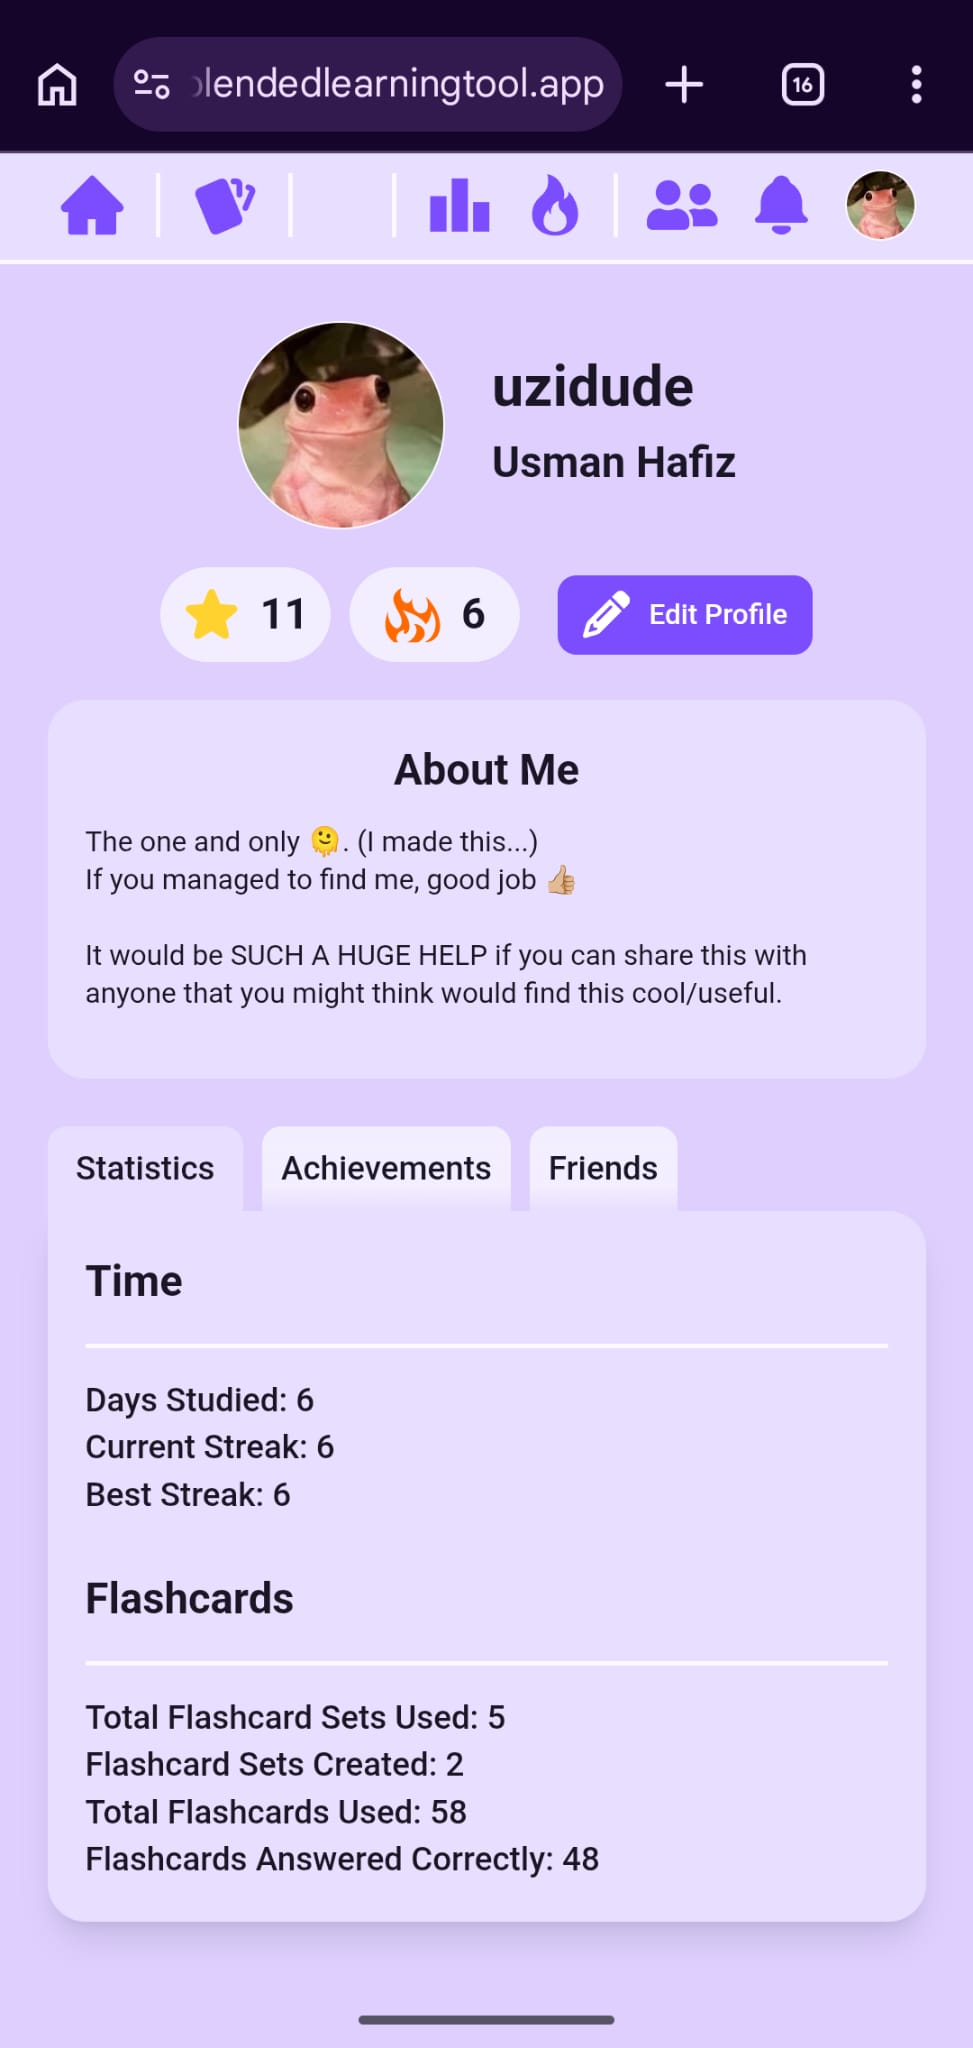
\includegraphics[width=0.9\linewidth, keepaspectratio]{Implementation/Mobile/MobileProfile.jpeg}
        \caption{Profile Page}
        \label{fig:mobileProfile}
    \end{subfigure}
    \caption{Some pages shown on mobile}
\end{figure}



\chapter{Evaluation}

This chapter details my methods of evaluating the effectiveness of ReviXion. \textcolor{magenta}{\textit{Add proper introduction. How...?}}

\section{Sharing ReviXion}

I want to give my users the most authentic experience possible when testing out ReviXion.
I did not want them to jump through hoops just to use it,
as this would decrease the likelihood of the test users to continue trying out the website as if it were a real application.
Therefore, I am using Vercel to host the website, as it is simple to use your existing GitHub repository.
At the time of writing, this website is running and available to use (blendedlearningtool.app).
\textcolor{magenta}{\textit{Is there a more elegant way of explaining that the website is still up and ready to use?}}
This way, it is very easy to share the link with potential test users so that they can try it out in their own time with minimal expectations required from them.

\subsection{Results}

\textcolor{magenta}{\textit{Discuss the numbers of the website (number of users, sets created, comments, etc)}}

\section{Google Form}

Alongside the link, I am also sending a Google Form that outlines general questions regarding their experience with the website.
\textcolor{magenta}{\textit{Discuss the reasoning behind the questions in the form?}}

\subsection{Results}

\textcolor{magenta}{\textit{Discuss the results of the google form}}

\section{Current Problems}

\subsection{UI Issues}

\textcolor{magenta}{\textit{Talk about how some users could not find features (delete individual flashcards) as well as the simplicity of the UI}}

\subsection{'Abusing the System'}

\textcolor{magenta}{\textit{Discuss abuse of the levelling system, spamming correct answers rewards more XP than it should}}

In future, implementing additional security checks as well as buffers would act to stop potential bad actors.

\begin{figure}[H]
    \centering
    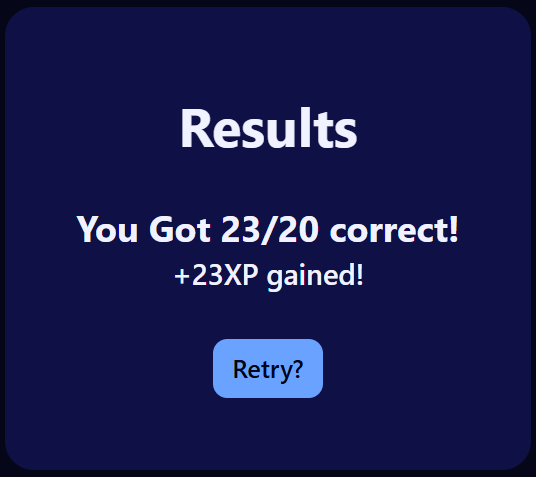
\includegraphics[width=0.4\linewidth]{Reflections/SpamCorrectExtraXP.png}
    \caption{An example of 'abusing the system', kindly provided by a test user. When using flashcards in 'Study Mode', pressing the 'correct' button in quick succession will bypass some checks and reward more XP than intended.}
    \label{fig:spamCorrectExtraXP}
\end{figure}

\section{Requested features}

\subsection{Flashcard Set Folders}

One piece of feedback regarded the organisation of flashcard sets.
Currently, users are given some filters to look through different sets.
However, if a user wanted to find a list of sets that pertain to one topic for example, they might struggle to do so if they solely rely on the search and tags.
Adding folders would mean that users could not only follow a 'series' of sets (such as multiple sets for individual topics of a course)
but also create their own folders to organise their flashcard sets.
This could be especially handy for university students, where the content of courses can change on a year to year basis and might require frequent updates.

\subsection{More Expressive Flashcards}

Multiple test users requested the ability to add images/diagrams to flashcards.
This would greatly benefit topics or subjects which are heavily reliant on diagrams, or would benefit users that find visual learning more useful for them.
Text decoration was another heavily requested feature, which would allow for bold text, italics, and different font sizes.
This would help to emphasise certain parts of the answer or give further explanation to questions.

\subsection{Further Study Methods}

Initially, I wanted to implement at least two forms of study tools, with the other being some form of quizzes.
Due to time constraints, I was not able to implement this alongside the flashcards.
However, as expected, one form of criticism regarded other forms of studying.
Adding quizzes to ReviXion would allow users to create their own questions that they can revisit,
as well as share with their friends to test each other.

A few test users also commented on their memories of Kahoot
and other forms of 'multiplayer learning'. \textcolor{magenta}{\textit{Find cite?}}
This leads into the idea of 'Parallel Play', which discusses how some people benefit from doing individual activities with other people.
This adds a sense of accountability and can help concentration levels. \textcolor{magenta}{\textit{Cite needed.}}
Adding this Kahoot-style quiz would allow users to form lobbies and compete with each other,
further maintaining their engagement with the website.

\subsection{Pomodoro Timer}

One test user described their struggles with studying due to their diagnosis of ADHD. \textcolor{magenta}{\textit{Cite needed.}}
A feature which has consistently helped them to concentrate is the pomodoro timer.
This is a method of studying whereby the user alternates between studying for some time (typically 30-60 minutes), and resting for some time (typically 5-10 minutes).
\textcolor{magenta}{\textit{Cite needed.}}
A future rendition of ReviXion would see the inclusion of this pomodoro timer,
which would persist between pages and maintain a history for short periods of inactivity.

\subsection{App Version}

Some users reported that they would like to see a version of the website as an app,
as they reported being drawn more to apps than having to go through their chosen browser.
\textcolor{magenta}{\textit{Find a statistic about people using apps/phones?}}
This would make it easier to keep users updated on notifications they receive on the website,
as well as help the user to maintain engagement with the app.
Giving users an option to use either of the website version or an app version would improve flexibility for each user's use case.

\section{Experiences from Test Users}

I wanted to dedicate a section for the different kinds of test users,
with their personal experiences and use cases for the website.

{\color{magenta}
\itshape
Zak: Engineering Course

Zainab: Social Anthropology

Sammy: Automotive Engineering

Khuloud's Friend: Tell this to developer:

Website flows smoothly very UX friendly really love it

Features are easy and simple to understand and follow

UI looks quite simple in fact a bit too simple but you know functions work well so whatever

When sending the code to user‘s email also allow showing the email it has been sent to so incase the user entered the wrong email they can figure out

Also when looking at achievements tab also allow a button to redirect the user to the proper page to achieve the named tasks

It was really nice to see so many users show interest in a study tool, regardless of age and education status.
}

\chapter{Reflections}

\section{Issues During Development}

\textcolor{magenta}{\textit{Discuss some of the personal issues that occured during development (spending too much time on smaller issues, the initial large scope of the project, and not being able to implement everything that I wanted)}}

\section{Organisation}

\textcolor{magenta}{\textit{Talk about git?}}

Throughout development, there were a couple of long periods of inactivity,
either due to burnout, or to focus on other work that required more attention.
It can be very overwhelming to try to get back into an existing project and relearn its codebase.
This includes remembering what needs tackling next, what solutions were already underway,
and any utilities that I had made that I can reuse moving forward.
Without tracking all of this information,
it would be very easy to revisit tasks that were already completed or remake solutions that I already had somewhere else in the codebase.

The Trello kanban board was a good solution for this, and greatly contributed to the success of the project.
It was very easy to write all of the information I wanted to in different categorised cards, so that I could revisit them at a later date.
By the end of development, 92 cards were created, of which, 81 of these cards were marked as completed.
This shows the necessity of using a tool to track your progress during the development of a project.

\section{A word on Generative AI}

Amidst the rise of generative AI and chatbots, 'vibe coding' is becoming more prevalent within the web development scene.
Whilst I understand the benefits of utilising generative AI during development, namely efficient coding,
it typically incurs a large 'code debt' that can snowball very quickly.
\textcolor{magenta}{\textit{Add a statistic? Potentially about the recent anthropic leak?}}
Additionally, core coding skills are being lost, and existing codebases are becoming littered with bugs and vulnerabilities.

Therefore, I leveraged generative AI in two exceptional cases.
Such cases include difficulties in debugging or planning the file hierarchy.
These are due to their minimal impact on the code itself, as well as time pressure given the nature and timescale of the project.
Specifically for debugging, I would heavily scrutinise any code that was generated to ensure I fully understood the reasoning behind the fix,
and typically rewrite the code myself.
This was done to minimise introducing any further bugs into the system and building up a 'code debt'.

This worked greatly in my favour.
I have developed a great understanding of my codebase, with clear, intentional semantics distinguishing each part of the website.
This hugely benefitted development, particularly near the end.
Each component of the codebase had its place,
and adding new features became as simple as slotting the pieces in the correct places.
Despite all of the setbacks and mistakes I made during development,
I have gained more of a deep understanding regarding web development, more so than I would have if I heavily relied on generative AI.
As a result, I can confidently say that this website is my own creation and something that I am proud to show off.

\section{Future Considerations}

In future, I want to dedicate more time to ReviXion.
As far as ReviXion has come, there are still plenty of flaws that can be improved on.
Aspects of the website like the levelling system and statistics could use some further consideration.
Also, whilst I have developed a lot of key skills when it comes to web development, there are still a lot of core principles that I wish to learn about.
Things such as security vulnerabilities and best practices for UX development are areas that I wish to improve on moving forward.

\textcolor{magenta}{\textit{Add a bit more}}

\section{Personal Reflection}

Speaking broadly, I am very pleased with what I have created.
What initially started as a simple prototype, turned into a production-ready study platform that has been well-received by testers.
It has been such a rewarding experience, not only to be able to bring an idea into fruition,
but also to see others show a genuine interest into the platform,
interacting with its various features and earnestly studying for their respective endeavours.

\textcolor{magenta}{\textit{Add a bit more}}

\end{document}